
\part{Measure}

% It might be useful to give a historical motivation for this course. Was it Lebesgue who wanted to see if there existed a consistent definition of length for arbitrary subsets of $\Bbb R$. It turns out the answer is no. Any extension of regular lengths on intervals violates some natural measures of length like, shift invariance and additivity, for example. We'll see this later when we define Lebesgue measure. To start, however, lets prove Borel's normal number theorem which extends the notion of length to a strange set, the set of normal numbers in $(0,1]$. We can prove the theorem in a elementary way and the result hints at a deeper theory. Side note, Borel's original proof contained a mistake and it wasn't corrected till Hausdorff in 1914 [check the facts here].



%%%%%%%%%%%%%%%%%%%%%%%%%%%%%%%%%%%%%%%%%%
%
% Section
%
%%%%%%%%%%%%%%%%%%%%%%%%%%%%%
\section{Borel's normal number theorem}
\label{Bsec}




\begin{definition}[{\bf Borel field}]
\label{fb}
Let $\mathcal B_0^{(0,1]}$ denote the class of finite (possibly empty) disjoint unions of intervals of the form  $(a,b]\subset (0,1]$.
\end{definition}

\begin{definition}
\label{l1defP}
Let $P$  be a probability assignment on $\mathcal B_0^{(0,1]}$ such that $P[(a,b]]=b-a$ for all $0\leq a\leq b\leq 1$ and extended to all of $\mathcal B_0^{(0,1]}$ using the identity $P[A\cup B]=P[A]+P[B]$ whenever $A,B$ are disjoint sets in $ \mathcal B_0^{(0,1]}$.
\end{definition}

\begin{theorem}
$P$ is well defined.
\end{theorem}


\begin{definition}
For each $\omega\in(0,1]$, let $d_k(\omega)$ denote the $k^\text{th}$ nonterminating binary digit of $\omega$. Let $z_k(\omega):=2d_k(\omega)-1$ and $s_n(\omega):=\sum_{k=1}^nz_k(\omega)\equiv\text{\rm excess of heads in $n$ tosses}$.
\end{definition}

\begin{theorem}[{\bf WLLN}]
For all $\epsilon>0$,
\begin{equation}
\label{Borel's WLLN}
\lim_{n\rightarrow \infty}P\Bigl[\bigl\{\omega\in (0,1]: \left|{s_n(\omega)}/n \right|\geq\epsilon \bigr\} \Bigr] =0.
\end{equation}
\end{theorem}
\begin{proof}
Notice first that any event or bet based on the values of $z_1(\omega), \ldots, z_n(\omega)$ must be a disjoint union of dyadic intervals of the form $(\frac{k-1}{2^n}, \frac{k}{2^n}]$. Therefore $\bigl\{\omega\in (0,1]: \left|{s_n(\omega)}/n \right| \geq \epsilon \bigr\} \in \mathcal B_0^{(0,1]}$ and the left hand side of (\ref{Borel's WLLN}) is well defined. Also notice
\begin{align*}
%\int_0^1 z_k(\omega)\, d\omega &= 0 \\
\int_0^1 z_k(\omega)z_j(\omega)\, d\omega
& = \begin{cases}
1 & \text{when $k=j$}\\
0 & \text{when $k\neq j$}.
\end{cases}
\end{align*}
This implies $\int_0^1 s^2_n(\omega)\, d\omega = \int_0^1 \sum_{k,j=1}^n z_k(\omega)z_j(\omega) \,d\omega = n$ which gives
\begin{align*}
n  &= \int_0^1 s^2_n(\omega)\, d\omega  \geq \int_{|s_n/n|\geq \epsilon} s^2_n(\omega)\, d\omega \\
& \qquad \geq \int_{|s_n/n|\geq \epsilon} n^2\epsilon^2\, d\omega  \geq n^2\epsilon^2 P\bigl[|s_n/n|\geq \epsilon\bigr]
\end{align*}
Therefore $P\bigl[|s_n/n|\geq \epsilon\bigr]\leq 1/(n\epsilon^2)\rightarrow 0$ as $n\rightarrow \infty$.
\end{proof}

\begin{definition}
The set of {\bf normal numbers} in $(0,1]$ is defined as
\begin{align*}
N
&:=\{\omega\in(0,1]: \lim_{n\rightarrow \infty} {s_n(\omega)}/n =0\}\\
&\phantom{:}=\{\omega\in(0,1]: \lim_{n\rightarrow \infty} \textstyle\frac{1}{n}\textstyle\sum_{k=1}^n d_k(\omega) = \textstyle\frac{1}{2}\}.
\end{align*}
The set of abnormal numbers is defined as $A:=(0,1]-N$.
\end{definition}


\begin{definition}[{\bf Negligible set}]
A subset $B\subset (0,1]$ is said to be {\bf negligible} if for all $\epsilon>0$, there exists $\mathcal B_0^{(0,1]}$-sets $B_1, B_2,\ldots$ such that
\begin{align*}
&B\subset \bigcup_{k=1}^\infty B_k\quad\text{and}\quad\sum_{k=1}^\infty P[B_k]\leq \epsilon.
\end{align*}
\end{definition}

\begin{theorem}[{\bf Borel's normal number theorem, i.e. the SLLN for coin flips}]
\label{thm: Borel's normal number theorem}
The set of abnormal numbers, $A$,  is negligible.
\end{theorem}
\begin{proof}
Let $\epsilon_k\downarrow 0$ as $k\rightarrow \infty$. Then
\begin{align}
\{\omega \colon |\textstyle\frac{s_{k^2}(\omega)}{k^2}| < \epsilon_k&\, \text{ for all large $k$} \} \nonumber\\
&\subset  \{\omega\colon \textstyle\lim_{k}\textstyle\frac{s_{k^2}(\omega)}{k^2} = 0 \}  \nonumber\\
&\subset \underbrace{\{\omega\colon \textstyle\lim_{n}\textstyle\frac{s_{n}(\omega)}{n} = 0 \}}_{= N}  \label{subseq for N}
\end{align}
To see why (\ref{subseq for N}) holds assume $\lim_k s_{k^2}(\omega)/\text{\scriptsize $k^2$} = 0$ for  $\omega$ and notice that
\newcommand{\tempn}{\text{\scriptsize $\lfloor\sqrt{n}\rfloor^2$}}
\begin{align*}
 \left|\frac{s_n}{n} \right| = \frac{|s_n|}{ (\sqrt{n})^{2} }
 \leq \frac{|s_n|}{\tempn} &\leq \frac{s_{\tempn}}{\tempn} + \frac{|s_n - s_\tempn|}{\tempn} \\
 & \leq \frac{s_{\tempn}}{\tempn} + \sum_{k = \tempn +1}^n \frac{|z_k|}{\tempn} \\
 & = {\frac{s_{\tempn}}{\tempn}} + \frac{(n-\tempn)}{\tempn} \longrightarrow 0
 \end{align*}
since $n-\tempn \leq (\text{\scriptsize $\lfloor\sqrt{n}\rfloor$} + 1)^2 - \tempn = 1 + 2\lfloor\sqrt{n} \rfloor $. Now by (\ref{subseq for N}) we have that
\begin{align*}
A = N^c  &\subset \{\omega \colon |\textstyle\frac{s_{k^2}(\omega)}{k^2}| \geq \epsilon_k\, \text{ for infinitely many $k$} \} \\
&\subset \bigcup_{k=j}^\infty  \underbrace{\{\omega \colon  |\textstyle\frac{s_{k^2}(\omega)}{k^2}| \geq \epsilon_k \}}_{=: B_k},\quad\text{for any $j$}
\end{align*}
where $B_k\in B_0^{(0,1])}$. By the proof of the WLLN we have
\[
P[B_k]\leq \frac{1}{k^2 \epsilon^2_k} = \frac{1}{k^{3/2}}
\]
when $\epsilon_k:= k^{-1/4}$. Therefore $\sum_{k=1}^n P[B_k]<\infty$ and hence $\sum_{k=j}^n P[B_k]\rightarrow 0$ as $j\rightarrow \infty$. Hence $A$ is negligible.
\end{proof}


\begin{exercise}
Using just calculus and ideas from this section, show that
\begin{equation}
\label{ex1a}
 M(t):= \int_0^1 e^{ts_n(\omega)}\,d\omega = \Bigl(\frac{e^t+e^{-t}}{2} \Bigr)^n
 \end{equation}
for each $t\in\Bbb R$. By differentiating with respect to $t$, show that $\int_0^1 s_n(\omega) \,d\omega = M^\prime (0)=0$ and $\int_0^1 s_n^2(\omega)\, d\omega =M^{\prime\prime} (0)=n$.
\end{exercise}

\begin{exerciseproof}
The idea is to split the integral $\int_0^1$ into the dyadic intervals of the form $(\frac{k-1}{2^n},\frac{k}{2^n} ]$. On each one of these intervals $s_n(\omega)$ is constant. Moreover, these intervals are in one-to-one correspondence with all $n-$digit binary digits. Therefore the dyadic intervals of order $n$ are then in one-to-one correspondence with $\{(z_1,\ldots, z_n)\colon z_k\in\{ -1,1\} \}$. Since $s_n(\omega) = z_1(\omega)+\cdots+ z_n(\omega) $ we have
\begin{align*}
\int_0^1 e^{ts_n(\omega)}\,d\omega
& = \sum_{k=0}^{2^n}\int_{(\frac{k-1}{2^n},\frac{k}{2^n} ]} e^{ts_n(\omega)}\,d\omega \\
& = \sum_{z_1=1,-1}\cdots  \sum_{z_n=1,-1}\frac{1}{2^n} e^{tz_1} \cdots e^{tz_n} \\
& = \Bigl(\sum_{z_1=1,-1}\frac{e^{tz_1}}{2}\Bigr)\cdots  \Bigl(\sum_{z_n=1,-1}\frac{e^{tz_n}}{2}\Bigr)\\
& = \Bigl(\frac{e^t+e^{-t}}{2} \Bigr)^n .
\end{align*}
\end{exerciseproof}



\begin{exercise}
\label{exp ineq for sn}
 Show that
\[P\bigl[|s_n/n|\geq \epsilon\bigr]\leq 2 e^{-n\epsilon^2/2}  \]
for each $\epsilon>0$.

 Hint: %$s_n(w)\geq n\epsilon$ entails $e^{ts_n(w)}\geq e^{tn\epsilon}$ for each $t>0$.
 Use (\ref{ex1a}) in conjunction with the inequality $(e^x + e^{-x})/2\leq \exp(x^2/2)$ which holds (why?) for all $x\in\Bbb R$.
\end{exercise}


%-------------------------------'
%---------section  ---------------'
%-------------------------------'
\clearpage
\section{Classes of sets}
%-------------------------------'
%---------section  ---------------'
%-------------------------------'

\subsection{Basic definitions}

\begin{definition}
$\Omega$ denotes the {\bf sample space}. Subsets of $\Omega$ are called {\bf events} and $2^\Omega$ denotes the power set of $\Omega$ (i.e. the class of all subsets of $\Omega$).
\end{definition}


\begin{definition}[{\bf field}] A collection of events $\mathcal F\subset 2^\Omega$  is a {\bf field} if
\begin{enumerate}
\item $\Omega\in \mathcal F$
\item $A\in\mathcal F\Longrightarrow A^c\in \mathcal F$
\item $A,B\in \mathcal F\Longrightarrow A\cup B\in \mathcal F$.
\end{enumerate}
\end{definition}



\begin{definition}[{\bf $\sigma$-field}]
A collection of events $\mathcal F\subset 2^\Omega$  is a {\bf $\sigma$-field} if
\begin{enumerate}
\item $\Omega\in \mathcal F$
\item $A\in\mathcal F\Longrightarrow A^c\in \mathcal F$
\item $A_1, A_2, \ldots \in \mathcal F\Longrightarrow \bigcup_{k=1}^\infty A_k \in \mathcal F$.
\end{enumerate}
\end{definition}




\begin{definition}[{\bf $\lambda$-system}]
A  collection of events $\mathcal F\subset 2^\Omega$ is called a {\bf $\lambda$-system} if
\begin{enumerate}
\item $\Omega\in \mathcal F$
\item $A\in\mathcal F\Longrightarrow A^c\in \mathcal F$
\item  $\underbrace{A_1, A_2, \ldots}_{\text{all disjoint}} \in \mathcal F \Longrightarrow \bigcup_{k=1}^\infty A_k \in \mathcal F$.
\end{enumerate}
\end{definition}

Notice that the only reason we require $\Omega\in \mathcal F$ in the definitions above is to force the class $\mathcal F$ be non-empty. We could just as well have changed the requirement $\Omega\in \mathcal F$ to the statment that there exists some $A\in \mathcal F$. One of the reasons it is traditional to put the assumption $\Omega\in \mathcal F$ is that the definition of a probability measure will require $P(\Omega)=1$. Therefore, it makes things more clear if we explicitly claim that $\Omega\in \mathcal F$, but otherwise its superfluous.


\begin{definition}[{\bf $\pi$-system}]
A  collection of events $\mathcal P\subset 2^\Omega$ is called a {\bf $\pi$-system} if
\begin{enumerate}
\item $A, B\in\mathcal P \Longrightarrow A\cap B\in\mathcal P$.
\end{enumerate}
\end{definition}




\begin{definition}[{\bf $A_n\uparrow A$}]
Let $A_1, A_2, \ldots$  and $A$ be events of $\Omega$. Then we write $\setlimup{n} A_n = A$ (or $A_n\uparrow A$) if
\begin{enumerate}
\item $A_1\subset A_2 \subset \cdots$
\item $A=\bigcup_{k=1}^\infty A_k$.
\end{enumerate}
\end{definition}

\begin{definition}[{\bf $A_n\downarrow A$}]
Let $A_1, A_2, \ldots$  and $A$ be events of $\Omega$. Then we write $\setlimdown{n} A_n = A$ (or $A_n\downarrow A$) if
\begin{enumerate}
\item $A_1\supset A_2 \supset \cdots$
\item $A=\bigcap_{k=1}^\infty A_k$.
\end{enumerate}
\end{definition}



\begin{definition}[{\bf monotone class}]
A collection of events $\mathcal M\subset 2^\Omega$  is a {\bf monotone class} if
\begin{enumerate}
\item $\Omega \in \mathcal M$
\item $A_1, A_2,\ldots\in\mathcal M$ and $A_n\uparrow A \Longrightarrow A\in\mathcal M$
\item $A_1, A_2,\ldots\in\mathcal M$ and $A_n\downarrow A \Longrightarrow A\in\mathcal M$.
\end{enumerate}
\end{definition}




\begin{theorem}[{\bf $\sigma = \lambda+\pi = \mathscr M + f$ }]
\begin{align}
\text{$\mathcal F$ is a $\sigma$-field}
&\Longleftrightarrow  \text{$\mathcal F$ is a field and a monotone class} \label{eq: m+f}\\
&\Longleftrightarrow  \text{$\mathcal F$ is a $\lambda$-system and a $\pi$-system.} \label{eq: l+p}
 \end{align}
\end{theorem}
\begin{proof}
({\sl show (\ref{eq: l+p})}) Notice the direction $(\Longrightarrow)$ is trivial. To show the other direction suppose $\mathcal F$ is a $\lambda$-system and a $\pi$-system. We need to show $\mathcal F$ is a $\sigma$-field. Notice $\Omega\in \mathcal F$ is trivial by $\lambda$-system properties. Also $A\in \mathcal F\Rightarrow A^c\in \mathcal F$ is trivial by $\lambda$-system properties. To show $A_1, A_2, \ldots \in \mathcal F\Rightarrow \cup_{k=1}^\infty\in \mathcal F$ one uses a common trick for turning a non-disjoint union into a disjoint union.
\begin{align*}
\bigcup_{k=1}^\infty A_k &= \bigcup_{k=1}^\infty \underbrace{A_k - (A_1\cup \cdots \cup A_{k-1})}_{disjoint} \\
 &= \bigcup_{k=1}^\infty A_k \cap A_1^c \cap \cdots \cap A_{k-1}^c
\end{align*}
Now $A_k^c \in \mathcal F$ by $\lambda$-system properties and hence $ A_k \cap A_1^c \cap \cdots \cap A_{k-1}^c\in \mathcal F$ by $\pi$-system properties. Therefore $\cup_{k=1}^\infty A_k$ can be written as a disjoint union of events from $\mathcal F$. Therefore $\cup_{k=1}^\infty A_k\in \mathcal F$ by $\lambda$-system properties as was to be shown.


({\sl show (\ref{eq: m+f})}) Just as in the proof of (\ref{eq: l+p}) the only non-trivial thing to show is that when $\mathcal F$ is a field and a monotone class this implies that $\mathcal F$ is closed under countable union. Indeed if $A_1, A_2, \ldots \in \mathcal F$ then
\[
\bigcup_{k=1}^\infty A_k = \setlimup{n} {\bigcup_{k=1}^n A_k}
\]
where ${\bigcup_{k=1}^n A_k}\in \mathcal F$ by the field properties and therefore $\bigcup_{k=1}^\infty A_k \in \mathcal F$ by the monotone class properties.

\end{proof}


\subsection{Generators}


\begin{theorem}[{\bf field generated by $\mathcal C$}]
Let $\mathcal C\subset 2^\Omega$. Then
\begin{equation}
\nonumber
f\langle\mathcal C \rangle := \bigcap_{\shortstack{\text{\small $\mathcal F$ is a field}  \\
 \text{\small $\mathcal C\subset \mathcal F$} }}\mathcal F
\end{equation}
is a field (which contains $\mathcal C$).
\end{theorem}


\begin{theorem}[{\bf $\sigma$-field generated by $\mathcal C$}]
Let $\mathcal C\subset 2^\Omega$. Then
\begin{equation}
%\label{eq: generating}
\nonumber
\sigma\langle\mathcal C \rangle := \bigcap_{\shortstack{\text{\small $\mathcal F$ is a $\sigma$-field}  \\
 \text{\small$\mathcal C\subset \mathcal F$ }}}\mathcal F
\end{equation}
is a $\sigma$-field (which contains $\mathcal C$).
\end{theorem}

\begin{theorem}[{\bf monotone class generated by $\mathcal C$}]
Let $\mathcal C\subset 2^\Omega$. Then
\begin{equation}
\nonumber
 \mathscr M\langle\mathcal C \rangle := \bigcap_{\shortstack{\text{\small $\mathcal M$ is a monotone class}  \\
 \text{\small$\mathcal C\subset \mathcal M$ }}}\mathcal M
\end{equation}
is a monotone class (which contains $\mathcal C$).
\end{theorem}






\begin{theorem}[{\bf $\lambda$-system generated by $\mathcal C$}]
Let $\mathcal C\subset 2^\Omega$. Then
\begin{equation}
\nonumber
\lambda\langle\mathcal C \rangle := \bigcap_{\shortstack{\text{\small $\mathcal L$ is a $\lambda$-system}  \\
 \text{\small$\mathcal C\subset \mathcal L$ }}}\mathcal L
\end{equation}
is a $\lambda$-system (which contains $\mathcal C$).
\end{theorem}




\begin{theorem}[{\bf Good sets}]
Let $\mathcal C$ and $\mathcal G$ be two collections of subsets of $\Omega$. If
\begin{itemize}
\item $\mathcal C\subset \mathcal G$;
\item $\mathcal G$ is a $\sigma$-field
\end{itemize}
Then  $\sigma\langle\mathcal C\rangle\subset \mathcal G$.
\end{theorem}


%%%%%%%%%%%%%%%%%%%%%%
\begin{theorem}[{\bf Restricted generators}]
\label{restricTHM}
Let $\Omega$ be a sample space and  $\mathcal C$ be a class of subsets of $\Omega$.  If $\Omega_0\subset \Omega$ then
\[
\underbrace{\sigma\bigl\langle  \mathcal C \cap \Omega_0 \bigr\rangle}_{\shortstack{ \text{\small $\sigma$-field} \\ \text{\small on $\Omega_0$}}}= \underbrace{\sigma\bigl\langle \mathcal C \bigr\rangle}_{\shortstack{ \text{\small $\sigma$-field} \\ \text{\small on $\Omega$}}} \cap\, \Omega_0.
\]
\end{theorem}

\begin{proof}
({\sl Show $\sigma \langle  \mathcal C \cap \Omega_0 \rangle \subset \sigma \langle \mathcal C  \rangle \cap\, \Omega_0$}) This easily follows by {\it good sets}  since clearly $\mathcal C\cap \Omega_0\subset \sigma\langle \mathcal C\rangle\cap \,\Omega_0$ and  Exercise \ref{sliceoutF} shows that $\sigma \langle \mathcal C  \rangle \cap\, \Omega_0$ is a $\sigma$-field.

({\sl Show  $\sigma\langle \mathcal C \rangle \cap\, \Omega_0 \subset \sigma \langle  \mathcal C \cap \Omega_0 \rangle $})  Notice that this inclusion is
equivalent to the statement that for every $A\in \sigma\langle\mathcal C\rangle$, $A\cap \Omega_0\in \sigma\langle\mathcal C\cap \Omega_0\rangle.$  To show this  let
\[ \mathcal G:=\{ A\subset \Omega: A\cap \Omega_0 \in \sigma\langle \mathcal C \cap \Omega_0 \rangle \}. \]
It will then be sufficient to show the following four bullets and then use good sets to conclude $\sigma\langle\mathcal C \rangle\subset \mathcal G$.
\\
\textbullet($\mathcal C\subset \mathcal G$)
$A\in \mathcal C \Longrightarrow A\cap \Omega_0\in \mathcal C \cap \Omega_0 \subset \sigma\langle \mathcal C \cap \Omega_0 \rangle.  $
\\
\textbullet($\Omega \in \mathcal G$)
\begin{align*}
\Omega_0\subset \Omega
&\Longrightarrow \Omega \cap \Omega_0 = \Omega_0 \in \sigma\langle \mathcal C\cap \Omega_0\rangle\\
&\qquad\qquad\text{since a  $\sigma$-field on $\Omega_0$ must contain $\Omega_0$} \\
&\Longrightarrow \Omega \in \mathcal G.
\end{align*}
\\
\textbullet($A\in \mathcal G\Longrightarrow A^c \in \mathcal G$) Notice that $A^c$  denotes complementation within $\Omega$. Now
\begin{align*}
A\in\mathcal G&\Longrightarrow A\cap \Omega_0\in \sigma\langle \mathcal C\cap \Omega_0\rangle \\
&\Longrightarrow \underbrace{\Omega_0-A\cap \Omega_0}_\text{\footnotesize complement in $\Omega_0$}\in \sigma\langle \mathcal C\cap \Omega_0\rangle \\
&\Longrightarrow \underbrace{\Omega_0\cap (A^c\cup \Omega_0^c)}_{= A^c\cap\Omega_0}\in \sigma\langle \mathcal C\cap \Omega_0\rangle \\
&\Longrightarrow A^c\in\mathcal G.
\end{align*}
\\
\textbullet($A_1,A_2,\ldots \in \mathcal G \Longrightarrow \bigcup_k A_k\in \mathcal G$)
\begin{align*}
A_1,A_2,\ldots \in \mathcal G&\Longrightarrow A_k\cap \Omega_0 \in \sigma\langle \mathcal C\cap \Omega_0\rangle,\,\forall k \\
&\Longrightarrow  \bigcup_k (A_k\cap \Omega_0) \in\sigma\langle \mathcal C\cap \Omega_0\rangle \\
 &\Longrightarrow  \Bigl(\bigcup_k A_k\Bigr)\cap \Omega_0 \in\sigma\langle \mathcal C\cap \Omega_0\rangle \\
&\Longrightarrow  \bigcup_k A_k\in \mathcal G.
\end{align*}
\end{proof}


\begin{theorem}[{\bf Halmos's monotone class theorem}]  If $\mathcal F_0$ is a field then $\mathscr M\langle \mathcal F_0\rangle = \sigma\langle \mathcal F_0\rangle$.
\end{theorem}


\begin{theorem}[{\bf Dynkin's $\pi - \lambda$ theorem}]  If $\mathcal P$ is a $\pi$-system then $\mathcal \lambda\langle \mathcal P\rangle = \sigma\langle \mathcal P\rangle$.
\end{theorem}
\begin{proof} This proof uses {\it good sets} all over the place.
First notice that  $\lambda\langle \mathcal P\rangle \subset \sigma\langle \mathcal P\rangle$ follows directly from {\it good sets} since $\mathcal P \subset \sigma\langle \mathcal P\rangle$ and clearly $ \sigma\langle \mathcal P\rangle$ is also a $\lambda$-system. Therefore we only need to show $\sigma\langle \mathcal P\rangle \subset \lambda\langle \mathcal P\rangle$.

Each statement below gives a sufficient condition to establish that $\sigma\langle \mathcal P\rangle \subset \lambda\langle \mathcal P\rangle$. They are given in reverse dependency order to make it easier to follow the train of reasoning.

\begin{quote}
\begin{centering}
$\sigma\langle \mathcal P\rangle \subset \lambda\langle \mathcal P\rangle$
 \\
$\Uparrow$
\\
$\lambda\langle\mathcal P\rangle$ is a $\sigma$-field
 \\
$\Uparrow$
\\
$\lambda\langle\mathcal P\rangle$ is a $\pi$-system
 \\
$\Uparrow$
\\
$\forall A, B\in \lambda\langle\mathcal P\rangle$ one has $ A\cap B\in \lambda\langle\mathcal P\rangle$
 \\
$\Uparrow$
\\
$\forall A \in \lambda\langle\mathcal P\rangle$ one has $\lambda \langle \mathcal P\rangle \subset \mathcal G_A$ where $\mathcal G_A:=\bigl\{ B\subset \Omega\colon A\cap B\in \lambda\langle \mathcal P\rangle \bigr\} $
\\
$\Uparrow$
\\
$\forall A \in \lambda\langle\mathcal P\rangle$, $\mathcal P\subset \mathcal G_A$ and $\mathcal G_A$ is a $\lambda$-system. \\
\end{centering}
\end{quote}
The last statement above is what we show. Notice, first, that
\begin{align}
\label{eq: l+d good set}
A\in \mathcal G_B \Longleftrightarrow A\cap B\in \lambda\langle \mathcal P\rangle \Longleftrightarrow B\in \mathcal G_A.
\end{align}
In particular if $A\cap B\in \lambda\langle\mathcal P\rangle$ then one has that both $A\in \mathcal G_B$ and $B\in \mathcal G_A$.


({\sl Case 1: show $\mathcal P\subset \mathcal G_A$ and $\mathcal G_A$ is a $\lambda$-system when $A\in \mathcal P$})
\\
\textbullet($\mathcal P\subset \mathcal G_A$) If $B\in \mathcal P$ then $A\cap B\in \mathcal P$ by the $\pi$-system properties of $\mathcal P$. Therefore $B\in \mathcal G_A$.
\\
\textbullet($\Omega\in \mathcal G_A$) This follows since $A\cap \Omega = A \in \mathcal P$.
\\
\textbullet($B\in \mathcal G_A\Longrightarrow B^c\in \mathcal G_A$)
\begin{align*}
B\in \mathcal G_A
&\Longrightarrow A\cap B\in \lambda\langle \mathcal P\rangle \\
&\Longrightarrow A - A\cap B\in \lambda\langle \mathcal P\rangle,\quad\text{$\lambda$-system properties} \\
&\Longrightarrow A -  B\in \lambda\langle \mathcal P\rangle \\
&\Longrightarrow A \cap  B^c\in \lambda\langle \mathcal P\rangle \\
&\Longrightarrow B^c\in \mathcal G_A.
\end{align*}
\\
\textbullet(disjoint $B_1, B_2, \ldots\in \mathcal G_A\Longrightarrow \cup_k B_k\in \mathcal G_A$)
Notice  $A \cap \bigcup_{k=1}^\infty B_k =  \bigcup_{k=1}^\infty (A \cap B_k)$. The $A\cap B_k$'s are disjoint if the $B_k$'s are too. Since $B_k$'s  are in $\mathcal G_A$, by assumption, we must have $A\cap B_k\in \lambda\langle \mathcal P\rangle$.
Therefore  $ \bigcup_{k=1}^\infty (A \cap B_k)\in \lambda\langle \mathcal P\rangle$ by $\lambda$-system properties.
Therefore $A \cap \bigcup_{k=1}^\infty B_k \in \mathcal G_A$.


({\sl Case 2: show $\mathcal P\subset \mathcal G_A$ and $\mathcal G_A$ is a $\lambda$-system when $A\in \lambda\langle\mathcal P\rangle$})
\\
\textbullet($\mathcal P\subset \mathcal G_A$) The only reason we established Case 1 was to proof this part of Case 2. Indeed,  Case 1 establishes that when $A\in \mathcal P$ we have that $\lambda\langle \mathcal P\rangle \subset \mathcal G_A$ by {\it good sets}. Changing names gives $\lambda\langle \mathcal P\rangle \subset \mathcal G_B$ whenever $B\in \mathcal P$. Now
\begin{align*}
B\in \mathcal P
&\Longrightarrow  \lambda\langle \mathcal P\rangle \subset \mathcal G_B,\quad\text{from Case 1}\\
&\Longrightarrow  A \in \mathcal G_B\\
&\Longrightarrow  B \in \mathcal G_A,\quad\text{by (\ref{eq: l+d good set}).}
\end{align*}
\\
\textbullet($\Omega\in \mathcal G_A$) Same as in Case 1.
\\
\textbullet($B\in \mathcal G_A\Longrightarrow B^c\in \mathcal G_A$) Same as in Case 1.
\\
\textbullet(disjoint $B_1, B_2, \ldots\in \mathcal G_A\Longrightarrow \cup_k B_k\in \mathcal G_A$) Same proof as in Case 1.


\end{proof}



\begin{theorem}[{\bf Good sets, take 2}]
Let $\mathcal P$ and $\mathcal G$ be two collections of subsets of $\Omega$. If
\begin{itemize}
\item $\mathcal P\subset \mathcal G$;
\item $\mathcal P$ is a $\pi$-system;
\item $\mathcal G$ is a $\lambda$-system
\end{itemize}
Then  $\sigma\langle\mathcal P\rangle\subset \mathcal G$.
\end{theorem}





%%%%%%%%%%%%%
\begin{exercise} \label{sliceoutF}
Suppose $\mathcal F$ is a $\sigma$-field on $\Omega$ and let $\Omega_0$ be any subset of $\Omega$ (not necessarily in $\mathcal F$). Prove that $\mathcal F\cap \Omega_0 := \{ F\cap \Omega_0: F\in \mathcal F\}$ is a $\sigma$-field on $\Omega_0$. \end{exercise}

\begin{exerciseproof}

\flushleft\textbullet({\sl Show $\Omega_0\in \mathcal F\cap \Omega_0$})
Notice that $\Omega \in \mathcal F$. Therefore $\Omega\cap \Omega_0\in \mathcal F\cap \Omega_0$. Now since $\Omega_0\subset \Omega$ implies $\Omega\cap\Omega_0= \Omega_0$ we have that $\Omega_0\in \mathcal F\cap \Omega_0$ as was to be shown.
\\
\textbullet({\sl Show $A\in \mathcal F\cap \Omega_0\Rightarrow (\Omega_0 - A)\in \mathcal F\cap \Omega_0$}) Let $A\in \mathcal F\cap \Omega_0$. Then $A = B\cap \Omega_0$ for some $B\in\mathcal F$. Therefore letting $A^c$ denote complementation within the larger space $\Omega$ we have
\begin{align*}
\Omega_0-A & = \Omega_0 \cap A^c\\
& =\Omega_0 \cap (B^c \cup \Omega_0^c)\\
& =\underbrace{\Omega_0 \cap B^c.}_{\in\mathcal F\cap \Omega_0}
\end{align*}
\\
\textbullet({\sl Show $A_1,A_2,\ldots \in \mathcal F\cap \Omega_0\Rightarrow \cup_{k=1}^\infty A_k\in \mathcal F\cap \Omega_0$}) Notice that each $A_k = B_k\cap \Omega_0$ for some $B_k\in\mathcal F$. Therefore
\begin{align*}
\bigcup_{k=1}^\infty A_k &=\bigcup_{k=1}^\infty (B_k\cap \Omega_0)\\
&=\Omega_0\cap \underbrace{\bigcup_{k=1}^\infty B_k}_{\mathcal F}
\end{align*}
Therefore $\bigcup_{k=1}^\infty A_k \in \mathcal F\cap \Omega_0$.
\end{exerciseproof}





\begin{exercise}
Prove Halmos's monotone class theorem. (Hint: To show $\sigma\langle \mathcal F_0 \rangle \subset \mathscr M\langle \mathcal F_0\rangle$ notice that it will be sufficient to show that $\mathscr M\langle \mathcal F_0\rangle$ is a field (why?); then to show  that $\mathscr M\langle \mathcal F_0\rangle$ is a field start by showing it is closed under complementation, then under intersection.)
\end{exercise}




\begin{exercise}
 \label{h2}
For any non-empty class $\mathcal A\subset 2^\Omega$, if
\begin{align*}
\mathcal C &:= \textit{the collection of $\mathcal A$ sets and their complements}\\
\mathcal I &:= \textit{the collection of finite intersections of $\mathcal C$ sets} \\
\mathcal U &:=\textit{the  collection of finite unions of $\mathcal I$ sets}.
\end{align*}
then $f\langle\mathcal A\rangle = \mathcal U$. Hint: first show $\mathcal U$ is closed under intersections, then complements.
\end{exercise}
\begin{exerciseproof}
We show $\mathcal U$  is a field and apply {\it good sets} to conclude $f\langle\mathcal A\rangle = \mathcal U$.


\flushleft\textbullet({\sl Show $\Omega \in \mathcal U$}) This is clear since $\mathcal C\subset \mathcal U$ and unions of two complimentary sets in  $\mathcal C$ sets gives $\Omega$.
\\
\textbullet({\sl Show $A,B\in \mathcal U\Longrightarrow A\cup B\in \mathcal U$}) This is trivial by definition of $\mathcal U$.
\\
\textbullet({\sl Show $A,B\in \mathcal U\Longrightarrow A\cap B\in \mathcal U$}) The general form of $\mathcal U$ sets can be written as follows (where $I_k\in\mathcal I$)
\begin{align*}
\underbrace{\bigcup_{k=1}^n I_k}_{\in \mathcal U}  \cap \underbrace{\bigcup_{j=n+1}^m I_{j}}_{\in \mathcal U} = \underbrace{\bigcup_{k=1}^n  \bigcup_{j=n+1}^m \underbrace{[I_{j}\cap I_{k}]}_{\in \mathcal I} }_{\in \mathcal U}
\end{align*}
since $\mathcal I$ is closed under intersection.
\\
\textbullet({\sl Show $A\in \mathcal U\Longrightarrow A^c\in \mathcal U$})
If $A\in \mathcal U$ then $A^c$ has the form
\[
\Bigl(\bigcup_{k=1}^n I_k \Bigr)^c = \bigcap_{k=1}^n I_k^c.
\]
where $I_k\in \mathcal I$ has the form $\cap_{j=1}^m C_j$ with $C_j\in \mathcal C$. Now notice that $I_k^c$ has the form $\cup_{j=1}^m C_j^c$ which is clearly in $\mathcal U$ since  $C_j^c\in\mathcal U$ and $\mathcal U$ is closed under union (by definition).
\end{exerciseproof}



\begin{definition}[{\bf Semi-ring with unit}]
A  collection of events $\mathcal A\subset 2^\Omega$ is called a {\bf semi-ring with unit} if
\begin{enumerate}
\item $\Omega\in \mathcal A$
\item $A, B\in\mathcal A\Longrightarrow A\cap B\in \mathcal A$
\item  If $A\in \mathcal A $ then $A^c$ is a finite disjoint union of $\mathcal A$-sets
\end{enumerate}
\end{definition}


\begin{exercise}
\label{ex: semi-ring}
Suppose $\mathcal A\subset 2^\Omega$ is a semi-ring with unit. Let $\mathscr D$ denote the class of finite disjoint unions of $\mathcal A$-sets. Show  $f\langle \mathcal A\rangle=\mathscr D$.
Hint: first show $\mathscr D$ is closed  intersections, then complements.
\end{exercise}
\begin{exerciseproof}

\textbullet({\sl Show $\mathcal A\subset \mathscr D$})
Trivial by definition of $\mathscr D$.
\\
\textbullet({\sl Show $\Omega\in \mathscr D$}) This follows since  $\Omega\in \mathcal A$.
\\
\textbullet({\sl Show $\mathscr D$ is closed under intersection})
Suppose $D, Q\in \mathscr D$. Then
\[
D\cap Q = \bigcup_{k=1}^n \bigcup_{j=1}^m A_k \cap  A_j^\prime
\]
where $A_k, A_j^\prime \in\mathcal A$, $A_1,\ldots, A_n$ are disjoint and $A_1^\prime,\ldots, A_n^\prime$  are disjoint. Therefore $A_k \cap  A_j^\prime$ are disjoint and are in $\mathcal A$ by property 2 of the semi-right-with-unit. Therefore $D\cap Q\in\mathscr D$ and therefore $\mathscr D$ is closed under intersection.
\\
\textbullet({\sl Show $\mathscr D$ is closed under complementation})
Let $D\in \mathscr D$. Clearly $D^c$ has the form $\cap_{i=1}^n A_i^c$ where $A_i\in \mathcal A$ are disjoint. But $A_i^c\in \mathscr D$ by property 3 of a semi-right-with-unit. Therefor $D^c= \cap_{i=1}^n A_i^c$ is in $\mathscr D$ since we already showed that $\mathscr D$ is closed under intersection.

The above bullets shows that $\mathscr D$ is a field which contains $\mathcal A$. Therefore $f\langle \mathcal A\rangle \subset \mathscr D$. To finish, simply notice that $\mathscr D\subset f\langle \mathcal A\rangle  $ by closure properties of a field.

\end{exerciseproof}




%%%%%%%%%%%%%
\begin{exercise} \label{stofB}
Show that  $\mathcal B_0^{(0,1]}$ from Definition \ref{fb} is a field and coincides with $f\langle (a,b]: 0\leq a\leq b\leq 1 \rangle $.
\end{exercise}

\begin{exerciseproof}
This should follow directly from exercise \ref{ex: semi-ring} and the fact that $\{ (a,b]: 0\leq a\leq b\leq 1 \}$ is a semi-ring with unit.
\end{exerciseproof}


\begin{exercise}
\label{ex1}
Let $\Omega = \Bbb R$.
Show that $f\langle (-\infty,a]: -\infty< a< \infty\rangle$  is the the set of finite (possibly empty) disjoint unions of intervals of the form $(-\infty, b]$, $(a,\infty)$ and $(a,b]$ for finite $a < b$. (Hint:  change the generators a bit to apply exercise \ref{ex: semi-ring}.)
\end{exercise}

\begin{exerciseproof}
  I think the easiest way to prove this is to use exercise \ref{ex: semi-ring}. In particular
\begin{align*}
f\langle (-\infty,a]:& -\infty< a< \infty\rangle \\
&= f\langle \underbrace{\varnothing, \Bbb R, (-\infty, b], (a,\infty), (a,b]\colon a < b}_{\text{semi-ring-with unit}} \rangle
\end{align*}

\end{exerciseproof}


\begin{exercise} \label{countablly generated}
Let $\mathcal A\subset2^\Omega$ be a countable collection of $\Omega$ sets.
Show that  $f\langle\mathcal A\rangle$ is a  countable collection of $\Omega$ sets.
\end{exercise}

\begin{exerciseproof}
Use  exercise \ref{h2}.
\end{exerciseproof}



\begin{exercise}
Let $\mathcal L$ be a collection of subsets of $\Omega$. Show that $\mathcal L$ is a $\lambda$-system if and only if $\mathcal L$ satisfies the following three conditions
\begin{enumerate}
\item $\Omega \in \mathcal L$
\item If $A-B\in \mathcal L$ whenever $B\subset A$ and $A, B\in \mathcal L$
\item $A_1, A_2,\ldots\in\mathcal L$ and $A_n\uparrow A \Longrightarrow A\in\mathcal L$.
\end{enumerate}
\end{exercise}

% %%%%%%%%%%%%%%%%%%
% \begin{definition}[{\bf Borel field}] The \underline{Borel field} on $(0,1]$, denoted $\mathcal B_0^{(0,1]}$, is defined as
% \[
%  f\bigl \langle (a,b] : 0\leq a < b\leq 1 \bigr\rangle
% \]
% (Note: by exercise \ref{stofB}  this does not conflict with definition \ref{fb}).
% \end{definition}


% %%%%%%%%%%%%%%%%%%%%%%%%%%%
% \begin{definition}[{\bf Borel $\sigma$-field}] The \underline{Borel $\sigma$-field} on $(0,1]$, denoted $\mathcal B^{(0,1]}$, is defined as
% \[
%  \sigma\bigl \langle (a,b] : 0\leq a < b\leq 1 \bigr\rangle.
% \]
% \end{definition}




\subsection{Borel $\sigma$-fields}
Borel $\sigma$-fields are used throught the whole theory of measure and integration. In this section we go into detail treatment of these fields. The main story is that Borel $\sigma$-fields have many equivenlent generators. Different generators are useful for proving different things. For example the Borel $\sigma$-field on $(0,1]^d$ as generated by the field of finite disjoint unions of rectangles is useful for constructing Lebesque measure. To specidfy uniqueness of a measure on $\Bbb R^d$ with a particular property it is often useful to consider the Broel field on $\Bbb R^d$ to be $\sigma\bigl\langle (-\infty,c_1]\times \cdots \times (-\infty, c_d]: -\infty < c_k< \infty \bigr\rangle$ the generators of which form a $\pi$-system.


\begin{definition}[{\bf Metric space Borel $\sigma$-field: $\mathcal B^\Omega$}]
Suppose $\Omega$ forms a metric space with some metric $d:\Omega\times\Omega\rightarrow [0,\infty]$. A set $A\subset \Omega$ is said to be {\bf open} if for each $x\in A$, there exists an $\epsilon>0$ such that the {open ball} $\{y\in\Omega: d(x,y)<\epsilon \}$ is contained in $A$. The {\bf Borel $\sigma$-field of $\Omega$} (with respect to metric $d$), denoted $\mathcal B^\Omega$, is defined as the $\sigma$-field generated by the open sets.
\end{definition}

The above definition immediately allows us to define the Borel $\sigma$-fields  $\mathcal B^{\Bbb R^d}$ and $\mathcal B^{(0,1]^d}$. To define $\mathcal B^{\bar{\Bbb R}^d}$ , where $\bar{\Bbb R}:=[-\infty, \infty]$ we use the metric given by $d(x,y):= |\tau(x) - \tau(y)|$ where
\begin{equation}
\label{eq: generate extended metric}
\tau(x):=\begin{cases} \frac{x}{1+|x|} &\text{ when $|x|<\infty$};\\
 1 &\text{when $x=\infty$};\\
  -1&\text{when $x=-\infty$}.
 \end{cases}
 \end{equation}



\begin{theorem}[{\bf Borel restrictions}]
Let $\Omega$ be a metric space and $\Omega_o\subset \Omega$.  Then the Borel $\sigma$-field $\mathcal B^{\Omega_o}$, which is constructed using the induced metric on $\Omega$, satisfies
\begin{align*}
\mathcal B^{\Omega_o} &=  \mathcal B^{\Omega}\cap \Omega_o
\end{align*}
If, in addition, $\Omega_o\in \mathcal B^{\Omega}$ then $\mathcal B^{\Omega_o}=  \{ B\in \mathcal B^\Omega: B\subset \Omega_o \}$.
\end{theorem}



\begin{proof}
({\sl Show $ \mathcal B^{\Omega_o} = \mathcal B^{\Omega}\cap \Omega_o$})
Let
\begin{align*}
\mathcal G &:= \text{open subsets of $\Omega$}\\
\mathcal G_o &:= \text{open subsets of $\Omega_o$}
\end{align*}
Notice that Theorem 2.30 in Rudin (Principles in Mathematical Analysis) shows that
\[ \mathcal G_o  = \mathcal G\cap \Omega_o.\]
This implies
\begin{align*}
\mathcal B^{\Omega_o}  = \sigma \langle \mathcal G_o\rangle &=  \sigma\langle \mathcal G \cap\Omega_o \rangle\\
& = \sigma\langle \mathcal G \rangle\cap \Omega_o,\,\,\text{by Theorem \ref{restricTHM}}\\
& = \mathcal B^{\Omega}\cap \Omega_o.
\end{align*}


({\sl Show $\mathcal B^{\Omega}\cap \Omega_o =  \{ B\in \mathcal B^\Omega: B\subset \Omega_o \}$ whenever $\Omega_o\in \mathcal B^{\Omega}$}). To see `$\supset$' suppose $B\subset \Omega_o$ and $B\in \mathcal B^\Omega$. Then $B = B\cap \Omega_o \in \mathcal B^{\Omega}\cap \Omega_o$. To  see `$\subset$' let $B\in  \mathcal B^{\Omega}\cap \Omega_o $ so that $B= \tilde B\cap \Omega_o$ where $\tilde B\in \mathcal B^\Omega$. Since $\Omega_o\subset \Omega$ we have $B\in \mathcal B^\Omega$ and $B\subset  \Omega_o $.
\end{proof}

% %%%%%%%%%%%%%%%%%%
% \begin{definition}[{\bf The Borel field on $(0,1]^d$}] The Borel field on $(0,1]^d$, denoted $\mathcal B_0^{(0,1]^d}$, is defined as the field generated by the rectangles in $(0,1]^d$ as follows
% \[
% \mathcal B_0^{(0,1]^d}:= f\bigl \langle (a_1,b_1]\times\cdots\times (a_d,b_d] : 0\leq a_k< b_k\leq 1 \bigr\rangle.
% \]
% \end{definition}


% %%%%%%%%%%%%%%%%%%%%%%
% \begin{theorem}[{\bf Structure of the Borel field on $(0,1]^d$}]
% \label{bfield}
% Any set in   $\mathcal B_0^{(0,1]^d}$ is a  finite (possibly empty) disjoint union of rectangles from $\{(a_1,b_1]\times\cdots\times (a_d,b_d] : 0\leq a_k< b_k\leq1  \}$.
% \end{theorem}

% %%%%%%%%%%%%%%%%%%%%%%%%%%%
% \begin{definition}[{\bf The Borel $\sigma$-field on $(0,1]^d$}]
%  The Borel $\sigma$-field on $(0,1]^d$, denoted $\mathcal B^{(0,1]^d}$, is defined as the field generated by the rectangles in $(0,1]^d$ as follows
% \[
% \mathcal B^{(0,1]^d}:= \sigma\bigl \langle (a_1,b_1]\times\cdots\times (a_d,b_d] : 0\leq a_k<b_k\leq 1 \bigr\rangle.
% \]
% \end{definition}


% %%%%%%%%%%%
% \begin{definition}[{\bf The Borel $\sigma$-field on $\Bbb R^d$}]
% The Borel $\sigma$-field of $\Bbb R^d$, denoted $\mathcal B^{\Bbb R^d}$, is defined as the $\sigma$-field generated by the class of all finite rectangles in $\Bbb R^d$ as follows
% \[ \mathcal B^{\Bbb R^d}:=\sigma\bigl\langle (a_1,b_1]\times \cdots \times (a_d,b_d]: -\infty< a_k<b_k<\infty \bigr\rangle. \]
% \end{definition}




\begin{theorem}[{\bf Non-exhaustive list of useful Borel generators}]\label{eqvgens}
\begin{align*}
\mathcal B^{\Bbb R^d}
& = \sigma\bigl\langle (-\infty,c_1]\times \cdots \times (-\infty, c_d]: -\infty < c_k< \infty \bigr\rangle    \\
& = \sigma\bigl\langle \text{open balls of $\Bbb R^d$}  \bigr\rangle  \\
& = \sigma\bigl\langle \text{open subsets of $\Bbb R^d$}  \bigr\rangle  \\
& = \sigma\bigl\langle \text{closed subsets of $\Bbb R^d$}  \bigr\rangle\\
& = \sigma\bigl\langle \text{compact subsets of $\Bbb R^d$}  \bigr\rangle \\
& = \sigma\bigl\langle \text{rectangles in $\Bbb R^d$}  \bigr\rangle \\
& = \sigma\bigl\langle \text{cylinders $\Bbb R^d$}  \bigr\rangle
\end{align*}
\begin{align*}
\mathcal B^{(0,1]}
&=\sigma\langle \mathcal B_0^{(0,1]}\rangle \hphantom{asdfdddddddasdfasdfasdfasdf}\\
&= \sigma\bigl\langle (a,b]: 0\leq a \leq b \leq 1 \bigr\rangle \\
  & =\sigma\bigl\langle (a,b): 0< a < b <1  \bigr\rangle \\
  & =\sigma\bigl\langle [a,b]: 0< a < b <1  \bigr\rangle \\
    & =\sigma\bigl\langle (0,a]: 0< a  <1  \bigr\rangle \\
& = \sigma\bigl\langle \text{open subsets of $(0,1]$}  \bigr\rangle  \\
& = \sigma\bigl\langle \text{closed subsets of $(0,1]$}  \bigr\rangle
\end{align*}
\begin{align*}
\mathcal B^{(0,1]^d}
& = \mathcal B^{\Bbb R^d}\cap (0,1]^d \\
& = \{B\in\mathcal B^{\Bbb R^d}: B\subset (0,1]^d  \} \\
&=  \sigma\bigl \langle (a_1,b_1]\times\cdots\times (a_d,b_d] : 0\leq a_k<b_k\leq 1 \bigr\rangle \\
& = \sigma\bigl\langle  \mathcal B_0^{(0,1]^d}  \bigr\rangle.
\end{align*}
where $\mathcal B_0^{(0,1]^d}:= f\bigl \langle (a_1,b_1]\times\cdots\times (a_d,b_d] : 0\leq a_k< b_k\leq 1 \bigr\rangle$ is the Borel field on $(0,1]^d$ which equals the finite (possibly empty) disjoint union of rectangles from $\{(a_1,b_1]\times\cdots\times (a_d,b_d] : 0\leq a_k< b_k\leq1  \}$

\end{theorem}

I would venture to say that one of the most important results above is that $\mathcal B^{(0,1]^d} = \sigma\bigl\langle  \mathcal B_0^{(0,1]^d}  \bigr\rangle$ where $\mathcal B_0^{(0,1]^d}$ is the field of finite (possibly empty) disjoint union of rectangles. This characterization allows one to construct probabilities on $\mathcal B_0^{(0,1]^d}$, then use the Carath\'eodory Extension Theorem to extend this to a full probability model on $\mathcal B^{(0,1]^d}$.

Notice that most of the equalities in Theorem \ref{eqvgens} are shown using the good sets principle. In particular, to show that $\sigma\langle \mathcal A_1\rangle=\sigma\langle\mathcal A_2 \rangle$ one simply needs to establish that $ \mathcal A_1 \subset \sigma\langle \mathcal A_2\rangle$ (which implies that $ \sigma\langle \mathcal A_1\rangle \subset \sigma\langle \mathcal A_2\rangle$ by ``good sets") and $ \mathcal A_2 \subset \sigma\langle \mathcal A_1\rangle$ (which implies that $ \sigma\langle \mathcal A_2\rangle \subset \sigma\langle \mathcal A_1\rangle$ by ``good sets").

\begin{proof}
I will only show one of these equalities. The rest follow by similar arguments.
To show
\[ \sigma\bigl\langle (a,b]: 0< a < b < 1 \bigr\rangle =\sigma\bigl\langle (a,b): 0< a < b <1  \bigr\rangle\]
it will be sufficient to show the following two statements for any arbitrary $0<a_0<b_0<1$.
\\
\textbullet({\sl Show $(a_0,b_0]\in \sigma\langle (a,b):0<a<b<1\rangle$})
This is follows from the identity
\[(a_0,b_0] = \bigcap_{n=1}^\infty (a_0,b_0+n^{-1} ).  \]
\\
\textbullet({\sl Show $(a_0,b_0)\in \sigma\langle (a,b]:0<a<b<1\rangle$})
This is follows from the identity
\[(a_0,b_0) = \bigcup_{n=1}^\infty (a_0,b_0-n^{-1}  ].  \]
\end{proof}

The sets in the Borel $\sigma$-field are extremely rich. In fact, it is hard to show that there are sets which are not in $\mathcal B^{\Bbb R}$. The easiest way to find such a set is to use properties of Lebseque measure which we will construct later in the notes. Therefore, we postpone a discussion of such sets until	 we have Lebseque measure at our disposal. For the reminder of this section we give some examples of sets which {\em are} in the Borel $\sigma$-fields on Euclidean space.

\begin{example}
The set of normal and abnormal numbers are in $\mathcal B^{(0,1]}$.
\end{example}


\begin{example}
All countable, co-countable (i.e. complements of countable sets), and perfect subsets of $(0,1]$ are in $\mathcal B^{(0,1]}$. In particular, the collection of  irrational numbers in $(0,1]$ is a Borel set.
\end{example}

\begin{example}
Show the Cantor set is an uncountable set in $\mathcal B^{(0,1]}$ (a nice way to see that it is uncountable is to work with a base-3 digit characterization of the Cantor set).
\end{example}


\begin{exercise}
Let $\Omega$ be a metric space with distance function $d$. $\Omega$ is said to be {\bf separable} if there exists a countable $\Omega_0\subset \Omega$ which is dense in $\Omega$ (i.e., every point of $\Omega$ is a limit of some sequence of points of $\Omega_0$).
\begin{enumerate}
\item Show that $\sigma\langle \text{open balls in $\Omega$}\rangle\subset \mathcal B^{\Omega}$.
\item Show that  $\sigma\langle \text{open balls in $\Omega$}\rangle= \mathcal B^{\Omega}$ if $\Omega$ is separable.
\item Show that $\Omega = \bar {\Bbb R}$ is separable with the metric defined with (\ref{eq: generate extended metric}) and conclude that $\sigma\langle \text{open balls in $\bar{\Bbb R}$}\rangle= \mathcal B^{\bar{\Bbb R}}$.
\end{enumerate}
\end{exercise}

\begin{exerciseproof}
({\sl Show 1.})
This is obvious since the open balls are also open sets (which generate $\mathcal B^{\Omega}$).

({\sl Show 2.})
It will be sufficient to show that the open sets can be constructed from a countable number of set operations on the open balls. Let $\Omega_0\subset \Omega$ be a dense subset.
Let $G$ be an open subset of $\Bbb R^d$. Now for each element $y\in G$ there exists an open ball $B_y$ centered at $y$ such that $B_y\subset G$. By the seperatbility there exists a $y_0\in \Omega_0$ close enough to $y$ such that there exists another open ball, call it $B_{y_0}$, for which  $y\in B_{y_0}\subset B_y$. Then clearly
\[
G = \bigcup_{y\in G} B_{y_0}.
\]
 Notice  there are only countably many elements in $\Omega_0$. Therefore the union $ \bigcup_{y\in G} B_{y_0}$ must be a countable union  and therefore $G$ can be constructed  from a countable number of set operations on the open balls, as was to be shown.


({\sl Show 3.}) Take the separable subset to be $\Bbb Q\cup \{ \infty\} \cup \{ -\infty\}$ where $\Bbb Q$ denotes the finite rationals. Notice there is an implicit application of continuity of $\tau$ here.
\end{exerciseproof}

\begin{exercise}
$\vphantom{aaa}$
\begin{enumerate}
\item Show that $\mathcal B^{\bar{\Bbb R}}$ is generated by the sets of the form $[-\infty, a]$ for $-\infty<a<\infty$, and also by sets of the form $[-\infty, a)$ for  $-\infty<a<\infty$.
\item Show that $\mathcal B^{\bar{\Bbb R}}$ is not generated by sets of the form $(-\infty, a)$ for $-\infty<a<\infty$. (Hint:  find a $\sigma$-field which contains the intervals $(-\infty, a)$ but which is strictly smaller than  $\mathcal B^{\bar{\Bbb R}}$ ).
\end{enumerate}
\end{exercise}
\begin{exerciseproof}
({\sl Show 1.})
Since ${\bar{\Bbb R}}$ is separable we can use the fact that $\mathcal B^{\bar{\Bbb R}}$  is generated by the open balls.
Therefore it is sufficient to show that $\mathcal F_1 = \mathcal F_2 = \mathcal F_3$ where
\begin{align*}
\mathcal F_1  & = \sigma\langle \text{open balls in $\bar{\Bbb R}$} \rangle\\
\mathcal F_{2} &= \sigma\langle [-\infty, a]\colon -\infty<a<\infty \rangle\\
\mathcal F_{3} &= \sigma\langle [-\infty, a)\colon -\infty<a<\infty   \rangle.
\end{align*}
Since each $\mathcal F_i$ is a $\sigma$-field we just have to show that one set of generators can construct the other set of generators, then apply {\it good sets}.
If $-\infty<a<\infty$ then
\begin{align*}
[-\infty, a] &= \bigcap_{n=1}^\infty [-\infty, a+\textstyle\frac{1}{n})  \\
[-\infty, a) &= \bigcup_{n=1}^\infty [-\infty, a-\textstyle\frac{1}{n}]
\end{align*}
which implies $\mathcal F_1 = \mathcal F_2$. Now notice that the open balls in $\bar{\Bbb R}$ have the form
$[-\infty, \infty],[-\infty, a),\, (b, a),\, (b, \infty] $
where  $-\infty<a<b<\infty$. Since these open balls contain the generators of $\mathcal F_3$ we immediately have $\mathcal F_3\subset \mathcal F_1$. The other inclusion easily follows by using the sets $[-\infty, a)$ to generate $(b, a),\, (b, \infty] $, thus showing that {\it open balls}$\,\subset \mathcal F_3$.

({\sl Show 2.}) Define
\[
\mathcal B_{-\infty, \infty}:= \mathcal B^{\Bbb R} \cup \bigl\{B\cup \{-\infty,\infty \}\colon B\in \mathcal B^{\Bbb R} \bigr\}
\]
and notice that it is easy/standard to show  $\mathcal B_{-\infty, \infty}$ is a $\sigma$-field. Since $\mathcal B_{-\infty, \infty}$ contains the sets $(-\infty, a)$ we have
\[ \sigma\langle  (-\infty, a)\colon -\infty<a<\infty \rangle\subset \mathcal B_{-\infty, \infty}\]
by {\it good sets}. Moreover
\[\mathcal B_{-\infty, \infty} \subsetneq  \mathcal B^{\bar{\Bbb R}} \]
since $\{\infty \}\in  \mathcal B^{\bar{\Bbb R}} $ but clearly $\{\infty \}\not\in  \mathcal B_{-\infty, \infty}  $.
\end{exerciseproof}




%
%%%%%%%%%%%%%%%%%%%
%\begin{exercise}
%Let $\Omega:=(0,1]$ and  let $\mathcal B(0,1]:= \sigma\langle (a,b]: 0< a <  b < 1 \rangle$. Show that
%\begin{align}
%\mathcal B(0,1] &= \sigma\bigl\langle (0,a]: 0< a < 1 \bigr\rangle \\
%& = \sigma\bigl\langle \text{open subsets of $(0,1]$}  \bigr\rangle
%\end{align}
%\end{exercise}
%

%\begin{exercise}  If $\Omega=[0,1]$ then
%\[\sigma\langle (0,a]: 0<a<1 \rangle \neq \sigma\langle [0,a]: 0<a<1 \rangle.\]
%However, if
% If $\Omega=(0,1]$ or  $\Omega=[0,1)$  or  $\Omega=(0,1)$ then
%\[\sigma\langle (0,a]: 0<a<1 \rangle = \sigma\langle [0,a]: 0<a<1 \rangle.\]
%This is just to show that you need to be a bit careful with the generators.
%\end{exercise}
%
%



\clearpage
%-------------------------------'
%---------section  ---------------'
%-------------------------------'
\section{Probability Measures}
%-------------------------------'
%---------section  ---------------'
%-------------------------------'


\begin{definition}[{\bf finitely additive probability}]
If $\mathcal F_0$ is a field on $\Omega$, then $P:\mathcal F_0\rightarrow [0,1]$ is said to be a {\bf finitely additive probability on $\mathcal F_0$} if
\begin{enumerate}
\item $P[\Omega]=1$
\item $P[A\cup B]=P[A]+P[B]$ \\ for all disjoint $A, B\in\mathcal F_0$.
\end{enumerate}
\end{definition}

Most of the basic rules of probability follow from  finitely additive properties.

\begin{theorem}[{\bf basic properties of finitely additive probabilities}]
Suppose $P$ is a  finitely additive probability on field $\mathcal F_0$. Then each of the following statements hold for all $\mathcal F_0$-sets $A, A_1, \ldots, B, B_1, \ldots$
\begin{enumerate}
\item $P[A^c] = 1-P[A]$;
\item $P[\varnothing]=0$;
\item\label{bpfa one} If $A\subset B$ then $P[B-A]=P[B]-P[A]$;
\item\label{bpfa two} {\bf (Increasing)} If $A\subset B$ then  $P[A]\leq P[B]$;
\item\label{bpfa three} {\bf (Inclusion-exclusion)} $P[A\cup B] = P[A]+P[B]-P[A\cap B]$;
\item\label{bpfa four} {\bf (Finite additivity)}  If $A_k$'s are disjoint then
\[ P\bigl[ \bigcup_{k=1}^n A_k \bigr] = \sum_{k=1}^n P[A_k]; \]
\item\label{bpfa five} {\bf (Finite sub-additivity)}
\[ P\bigl[ \bigcup_{k=1}^n A_k \bigr] \leq \sum_{k=1}^n P[A_k]; \]
\item\label{bpfa six} {\bf (Approximation)} If $A_k\subset B_k$ then
\begin{align*}
P\bigl[ \bigcup_{k=1}^n B_k \bigr] - P\bigl[ \bigcup_{k=1}^n A_k \bigr] &\leq \sum_{k=1}^n P[B_k - A_k] \\
P\bigl[ \bigcap_{k=1}^n B_k \bigr] - P\bigl[ \bigcap_{k=1}^n A_k \bigr] &\leq \sum_{k=1}^n P[B_k - A_k].
\end{align*}
\end{enumerate}
\end{theorem}
\begin{proof}
\textbullet({\sl Show item \ref{bpfa one}}) If $A\subset B$ then $B = A \cup (B-A)$ is a disjoint union. Therefore $P[B] = P[A] + P[B-A]$ which implies $P[B-A]=P[B]-P[A]$.
\\
\textbullet({\sl Show item \ref{bpfa two}}) Use $0\leq P[B-A]=P[B]-P[A]$.
\\
\textbullet({\sl Show item \ref{bpfa three}}) Use the fact that $A\cup B$ can be written as a disjoint union ${A \cup (B-A\cap B)}$ to get that
\begin{align*}
P[A\cup B]&= P[A] + P[B-A\cap B] \\
&= P[A] + P[B] - P[A\cap B].
\end{align*}
\\
\textbullet({\sl Show item \ref{bpfa four}}) Use induction.
\\
\textbullet({\sl Show item \ref{bpfa five}}) Use induction and inclusion exclusion.
\\
\textbullet({\sl Show item \ref{bpfa six}})
For the first equation use the fact that $\cup_k B_k - \cup_k A_k$ and $\cap_k B_k - \cap_k A_k$  are covered by $\cup_k(B_k - A_k)$ and then apply sub-additivity.

\end{proof}

\begin{definition}[{\bf probability measure}]
If $\mathcal F_0$ is a field on $\Omega$, then $P:\mathcal F_0\rightarrow [0,1]$ is said to be a {\bf probability measure on $\mathcal F_0$} if
\begin{enumerate}
\item $P(\Omega)=1$
\item $P\bigl( \bigcup_{k=1}^\infty A_k \bigr)=\sum_{k=1}^\infty P(A_k)$ \\ for all disjoint $A_1, A_2,\ldots \in\mathcal F_0$ such that $\bigcup_{k=1}^\infty A_k \in \mathcal F_0$.
\end{enumerate}
\end{definition}

The following theorem tells us that a consequences of the countable additivity which do not follow from finite additivity.


\begin{theorem}[{\bf Countable additivity equivalence}]
\label{thm: cae}
Let $P:\mathcal F_0\rightarrow [0,1]$ be a finitely additive probability on a field $\mathcal F_0$. Then the following statements are equivalent:
\begin{enumerate}
\item $P$ is a probability measure;
\item ({\bf Continuous from below}) If whenever $A_1, A_2, \ldots \in \mathcal F_0$ and $A_n\uparrow A\in\mathcal F_0$ then $P(A_n)\uparrow P(A)$;
\item ({\bf Continuous from above})  If whenever $A_1, A_2, \ldots \in \mathcal F_0$ and $A_n\downarrow A\in\mathcal F_0$ then $P(A_n)\downarrow P(A)$;
\item ({\bf Continuous from above at $\varnothing$}) If whenever $A_1, A_2, \ldots \in \mathcal F_0$ and $A_n\downarrow  \varnothing$ then $P(A_n)\downarrow 0$.
\end{enumerate}
\end{theorem}
\begin{proof}
({\sl 1. $\Longrightarrow $ 2.}) Assume $A_1, A_2, \ldots \in \mathcal F_0$ and $A_n\uparrow A\in\mathcal F_0$. Then
 \begin{align*}
 P[A_n] &= P\Bigl[ \textstyle\bigcup_{k=1}^n A_k \Bigr],\qquad\text{since $A_1\subset A_2\subset \cdots$}\\
 &= P\Bigl[ \textstyle\bigcup_{k=1}^n \underbrace{\{A_k - (A_{k-1}\cap \cdots \cap A_1)\}}_{\text{disjoint}} \Bigr] \\
 &= \textstyle\sum_{k=1}^nP\Bigl[ \{A_k - (A_{k-1}\cap \cdots \cap A_1)\} \Bigr] \\
 &\uparrow \textstyle\sum_{k=1}^\infty P\Bigl[ \{A_k - (A_{k-1}\cap \cdots \cap A_1)\} \Bigr] \\
 &=P\Bigl[ \textstyle\bigcup_{k=1}^\infty \{ A_k - (A_{k-1}\cap \cdots \cap A_1)\} \Bigr],\,\,\text{by item 1.}\\
 &=P[ A ]
 \end{align*}


({\sl 2. $\Longrightarrow $ 1.}) The only thing to show is countable additivity over disjoint sets which stay in the field. In paritcular suppose $A_1, A_2, \ldots $ are disjoint $\mathcal F_0$-sets  such that $\textstyle\bigcup_{k=1}^\infty A_k \in \mathcal F_0$. Then
\begin{align*}
P\Bigl[\textstyle\bigcup_{k=1}^\infty A_k \Bigr]= P\Bigl[\setlimup{n}\textstyle\bigcup_{k=1}^n A_k \Bigr] = \setlimup{n}P\Bigl[\textstyle\bigcup_{k=1}^n A_k \Bigr]
 \end{align*}
 where the last equality follows by assuming item 2.


 ({\sl 2. $\Longleftrightarrow $ 3.}) Use the fact that $A_n\uparrow A \Longleftrightarrow A_n^c \downarrow A^c$ along with the identity $P[A] = 1- P[A^c]$.


 ({\sl 3. $\Longrightarrow $ 4.}) This is clear since $P[\varnothing ]=0$

 ({\sl 4. $\Longrightarrow $ 3.}) Suppose $P$ is continuous from above at $\varnothing$. Now suppose  $A_1, A_2, \ldots \in \mathcal F_0$ and $A_n\downarrow A\in\mathcal F_0$. Now to show item 3 notice
 \begin{align*}
 A_n\downarrow A
 &\Longrightarrow A_n-A \downarrow \varnothing \\
 &\Longrightarrow P[A_n]-P[A] = P[A_n-A]   \downarrow 0,\,\,\text{by item 4.} \\
 &\Longrightarrow P[A_n] \downarrow P[A]  \\
 \end{align*}
\end{proof}

\begin{theorem}[{\bf Countable sub-additivity}]
Let $P$ be a probability measure on a field $\mathcal F_0$. If $A_1, A_2, \ldots$ are $\mathcal F_0$-sets for which $\bigcup_{k=1}^\infty A_k\in \mathcal F_0$. Then
\[ P\Bigl[\textstyle\bigcup_{k=1}^\infty A_k \Bigr]\leq \sum_{k=1}^\infty P\bigl[A_k \bigr]. \]
\end{theorem}
\begin{proof}
\begin{align*}
 P\Bigl[\textstyle\bigcup_{k=1}^\infty A_k \Bigr]
 & =  P\Bigl[\setlimup{n}\textstyle\bigcup_{k=1}^n A_k \Bigr] \\
 & =  \setlimup{n} P\Bigl[\textstyle\bigcup_{k=1}^n A_k \Bigr],\,\text{continuity from below}\\
 & \leq  \setlimup{n} \textstyle\sum_{k=1}^n P\bigl[A_k \bigr],\,\text{finite sub-additivity}\\
 & =  \textstyle\sum_{k=1}^\infty P\bigl[A_k \bigr].
\end{align*}
\end{proof}


%%%%%%
\begin{theorem}
\label{thm: Borels P is a measure}
 The mapping $P:\mathcal B_0^{(0,1]}\rightarrow [0,1]$ defined in Definition \ref{l1defP} is a probability measure.
 \end{theorem}
\begin{proof}
We will use Theorem \ref{thm: cae} and show that $P$ is continuous from above at $\varnothing.$ Let $A_n \downarrow \varnothing$ where $A_n\in \mathcal B_0^{(0,1]}$ (in particular we have that $\bigcap_{k=1}^\infty A_k =\varnothing$). We show $P[A_n]\downarrow 0$.

Notice first that for all $n\geq N$ we have
\[ P[A_n]\leq P[A_N] =  P\bigl[ \textstyle\bigcap_{k=1}^N A_k\bigr] \]
since the $A_k$'s are decreasing. It will then be sufficient to show that for all $\epsilon>0$ there exists  $N_\epsilon$ such that
\begin{equation}
\label{eq: show pm for bo}
P\bigl[ \textstyle\bigcap_{k=1}^{N_\epsilon} A_k\bigr]\leq \epsilon.
\end{equation}

The following argument doesn't quite work but it will motivate the solution. Let $\epsilon > 0$ and for each $A_k$  find a sequence of closed sets $F_k$ such that $F_k\subset A_k$ and $P[A_k-F_k]\leq \epsilon/2^k$ (If $A_k$ has the form $\bigcup_i (a_i,b_i]$ take $F_k:=\bigcup_i [a_i+\tau,b_i]$ for small enough $\tau$). Since $\bigcap_{k=1}^\infty A_k=\varnothing$ one has that $\bigcap_{k=1}^\infty F_k=\varnothing$.
By a compactness argument\footnote{For, if not, then there exists $x_n\in \bigcap_{k=1}^n F_k$ for each $n$. Notice
\begin{equation}
\label{foot:main eq}
\text{$\bigcap_{k=1}^n F_k\subset \bigcap_{k=1}^m F_k$ when $m\leq n$}
\end{equation}
For one thing, equation (\ref{foot:main eq}) implies that $x_n\in F_1$. Therefore by compactness  there exists a  sub-sequential limit $x=\lim_k x_{n_k} \in F_1$.  Again by (\ref{foot:main eq}) and the assumption  $x_{n_k}\in \bigcap_{k=1}^{n_k} F_k$ one has that for sufficiently large $k$ all  $x_{n_k}$ are eventually within $F_m$. Therefore $x\in F_m$ for each $m$. This contradicts the assumption $\cap_{k=1}^\infty F_k=\varnothing$.  } there exists an $N_\epsilon$ such that $\bigcap_{k=1}^{N_\epsilon} F_k=\varnothing$.
 Therefore
\[
P\bigl[ \textstyle\bigcap_{k=1}^{N_\epsilon} A_k\bigr] - \underbrace{P\bigl[ \underbrace{\textstyle\bigcap_{k=1}^{N_\epsilon} F_k}_{=\varnothing}\bigr]}_{=0}\leq  \sum_{k=1}^{N_\epsilon} P\bigl[A_k-F_k \bigr] \leq \sum_{k=1}^{N_\epsilon} \frac{1}{2^k}\leq \epsilon.
\]
This would establish (\ref{eq: show pm for bo}) if it weren't for the problem that $P$ isn't defined on the $F_k$'s.

It is clear how to fix this. For each $A_k$ find  closed sets $F_k$ and $\mathcal B_0^{(0,1]}$-sets $A_k^o$ such that $A_k\supset F_k \supset A_k^o$ and $P[A_k-A_k^o]\leq \epsilon / 2^k$. For each $\epsilon>0$ we still have the property that there exists $N_\epsilon$ such that  $\bigcap_{k=1}^{N_\epsilon}F_k = \varnothing$ which  implies $\bigcap_{k=1}^{N_\epsilon}A^o_k = \varnothing$  and now
\[
P\bigl[ \textstyle\bigcap_{k=1}^{N_\epsilon} A_k\bigr] - \underbrace{P\bigl[ \underbrace{\textstyle\bigcap_{k=1}^{N_\epsilon} A^o_k}_{=\varnothing}\bigr]}_{=0}\leq  \sum_{k=1}^{N_\epsilon} P\bigl[A_k-A^o_k \bigr] \leq \sum_{k=1}^{N_\epsilon} \frac{1}{2^k}\leq \epsilon.
\]
\end{proof}



\clearpage
%-------------------------------'
%---------section  ---------------'
%-------------------------------'
\section{Carath\'eodory Extension Theorem}
%-------------------------------'
%---------section  ---------------'
%-------------------------------'

%%%%%%%%%%%%%%%%%
\begin{theorem}[{\bf Uniqueness for probability measures}]
\label{ui}
Let $\mathcal P$ be a collection of subsets of $\Omega$.
If $P$ and $Q$ are two probability measures on $(\Omega, \sigma\langle \mathcal P\rangle)$ such that
\begin{enumerate}
\item $P$ and $Q$ agree on $\mathcal P$;
\item $\mathcal P$ is a $\pi$-system,
\end{enumerate}
then $P$ and $Q$ agree on all of $ \sigma\langle \mathcal P\rangle$.
\end{theorem}
\begin{proof}
This is our first use of Dynkin's $\pi-\lambda$ theorem which allows us to extend the good sets principle. In particular, define the good sets as follows:
\begin{equation}
\mathcal G:=\{A\subset \Omega\colon Q[A] = P[A] \}.
\end{equation}
Dynkin's $\pi-\lambda$ theorem says that $\sigma\langle \mathcal P\rangle = \lambda\langle \mathcal P\rangle$ since $\mathcal P$ is a $\pi$-system. Therefore to show $\sigma\langle \mathcal P\rangle = \lambda\langle \mathcal P\rangle\subset \mathcal G$ we just show that $\mathcal G$ is a $\lambda$-system and invoke {\it good sets}.

\textbullet({\sl $\Omega \in \mathcal G$}) This is trivial since $Q[\Omega]=1$ and $P[\Omega]=1$  by properties probability measures.
\\
\textbullet({\sl $A\in \mathcal  G\Longrightarrow A^c\in \mathcal G$})
\begin{align*}
A\in \mathcal G
&\Longrightarrow Q[A] = P[A]  \\
&\Longrightarrow 1-Q[A^c] = 1-P[A^c] \\
&\Longrightarrow Q[A^c] = P[A^c] \\
&\Longrightarrow A^c\in \mathcal G.
\end{align*}
\\
\textbullet({\sl disjoint $A_1, A_2\in \mathcal  G\Longrightarrow \bigcup_{k=1}^\infty A_k\in \mathcal G$})
\begin{align*}
\underbrace{A_1,A_2,\ldots}_{\text{disjoint}}\in \mathcal G
&\Longrightarrow  Q[A_k] = P[A_k],\,\forall k  \\
&\Longrightarrow \underbrace{\sum_{k=1}^\infty Q[A_k]}_{=Q[\cup_{k=1}^\infty A_k]} = \underbrace{\sum_{k=1}^\infty P[A_k]}_{=P[\cup_{k=1}^\infty A_k]}  \\
&\Longrightarrow \bigcup_{k=1}^\infty \in \mathcal G.
\end{align*}
Notice that this last statement could not be proved if the $A_k$'s were not disjoint. This illustrates the necessity of Dynkin's $\pi-\lambda$ theorem.

\end{proof}


\begin{sectionassumption}
\label{outer}
For the remainder of this section $P_0$ denotes a probability measure on $\mathcal F_0$, where $\mathcal F_0$ is a field on $\Omega$. Also let $\mathcal F^\uparrow, \mathcal F^\downarrow,  \bar{\mathcal F}, P^\uparrow, P^\downarrow, P^*, P_*, \bar P$ be defined as follows
\begin{itemize}
\item  $\mathcal F^\uparrow := \{\setlimup{k}  A_k : A_k\in \mathcal F_0  \}$
\item  $\mathcal F^\downarrow := \{\lim_k\!\!\downarrow A_k : A_k\in \mathcal F_0  \}$
\item $P^\uparrow(\lim_k\!\!\uparrow A_k) := \lim_k P_0(A_k)$  when $\lim_k\!\!\uparrow A_k\in \mathcal F^\uparrow$
\item $P^\downarrow(\lim_k\!\!\downarrow A_k) := \lim_k P_0(A_k)$ when  $\lim_k\!\!\downarrow A_k\in \mathcal F^\downarrow$
\item  $P^*(A):=\inf\{P^\uparrow(A^\uparrow): A\subset A^\uparrow\in \mathcal F^\uparrow  \}$ when $A\in2^\Omega$
\item $P_*(A):=\sup\{P^\downarrow(A^\downarrow): A\supset A^\downarrow\in \mathcal F^\downarrow  \}$ when $A\in2^\Omega$
\item  $\bar{\mathcal F}:=\{ A\in 2^\Omega : P^*(A) = P_*(A)\}$
\item $\bar P(A):=P^*(A)=P_*(A)$ when $A\in \bar{\mathcal F}$
%\item $\mathcal F :=\sigma\langle \mathcal F_0 \rangle$. Note: we will show $\mathcal F\subset \overline{\mathcal F}$.
%\item $P(A):= \overline P(A)$ for all $A\in \mathcal F$.
\end{itemize}
\end{sectionassumption}



\begin{theorem}
\label{thm: well defined Pup, P*}
 $P^\uparrow$, $P^\downarrow$, $P^*$ and $P_*$ are all well defined. Moreover,  $(2^\Omega, P^*)$ is an extension of $(\mathcal F^\uparrow, P^\uparrow)$ which is an extension of $(\mathcal F_0, P_0)$ (and similarly for $(2^\Omega, P_*)$ and $(\mathcal F^\downarrow, P^\downarrow)$).
 \end{theorem}
\begin{proof}
({\sl Show $P^\uparrow$ is well defined})
Notice that if $A_n \uparrow A$ then  $\lim_n P_0[A_n]$ exists by monotonicity and boundedness of $P_0[A_n]$. Therefore we just need to show that  $\lim_n P_0[A_n] = \lim_n P_0[B_n]$ whenever $\setlimup{n} A_n =  \setlimup{n} B_n$.
It will be sufficient to show that for any $A_n, B_n\in \mathcal F_0$ we have
\begin{equation}
\label{eq: increasing Pup}
\setlimup{n} A_n \subset   \setlimup{n} B_n \Longrightarrow \lim_n P_0[A_n] \leq \lim_n P_0[B_n].
\end{equation}
Notice that if $\setlimup{n} A_n \subset   \setlimup{n} B_n$ then
$A_n = A_n \cap \bigl(\setlimup{m} B_m\bigr) =  \setlimup{m} (A_n\cap B_m).
$
Therefore
\begin{align*}
P_0[A_n]  & = P_0\bigl[\setlimup{m} \underbrace{(A_n\cap B_m)}_{\in \mathcal F_0}\bigr] \\
& = \setlimup{m} P_0 [(A_n\cap B_m)],\quad\text{since $P_0$ is a prob measure} \\
& \leq  \setlimup{m} P_0[B_m].
\end{align*}
Now taking limits of both sides in $n$ gives $\setlimup{n}P_0[A_n]\leq  \setlimup{m} P_0\bigl[B_m\bigr]$ as was to be shown. Notice that (\ref{eq: increasing Pup}) implies  increasingness of $P^\uparrow$. In particular
\begin{equation}
\label{eq: increasing Pup II}
\text{$A^\uparrow, B^\uparrow \in \mathcal F^\uparrow$ and  $A^\uparrow\subset B^\uparrow$}
 \Longrightarrow P^\uparrow[A^\uparrow]\leq P^\uparrow[B^\uparrow].
\end{equation}


({\sl Show $(\mathcal F^\uparrow, P^\uparrow)$ extends $(\mathcal F_0, P_0)$})
We need to show that $\mathcal F_0\subset \mathcal F^\uparrow$ and $P^\uparrow = P_0$ on $\mathcal F_0$.
Clearly $\mathcal F_0\subset \mathcal F^\uparrow$ holds since  any $A\in \mathcal F_0$ can be trivially written as $A = \setlimup{n} A$. The second statement follows since whenever $A\in \mathcal F_0$ we have that
\begin{equation}
P^\uparrow[A] := \setlimup{n}P_0[A] = P_0[\setlimup{n}A] =   P_0[A]
\end{equation}
where the second equality follows since we are assuming $P_0$ is a probability measure.



({\sl Show $P^*$ is well defined}) Trivial.


({\sl Show $(2^\Omega, P^*)$ extends $(\mathcal F^\uparrow, P^\uparrow)$}) Trivially we have $\mathcal F^\uparrow \subset 2^\Omega$. Also notice that  if $A \in \mathcal F^\uparrow$ then
\begin{align*}
P^\uparrow(A) &\leq \underbrace{\inf\{P^\uparrow(A^\uparrow): A\subset A^\uparrow\in \mathcal F^\uparrow  \}}_{ = P^*[A]} \leq P^\uparrow(A).
\end{align*}
where the first inequality is given by (\ref{eq: increasing Pup II}) and the second inequality follows since $A\subset A\in \mathcal F^\uparrow$ is one of the covers in the infimum.

The proofs for $(\mathcal F^\downarrow, P^\downarrow)$ and $(2^\Omega, P_*)$ follow in a similar manner (after noticing $A_n\uparrow A \Longleftrightarrow A_n^c \downarrow A^c$).

\end{proof}


\begin{theorem}[{\bf 5 facts about $P^*$ and $P_*$}]
\label{f5}
For all sets $A, B,C, A_1, \ldots\in 2^\Omega$
\begin{enumerate}
\item\label{eff1}  $P^* (A) + P_*(A^c) = 1$.
\item\label{eff2}  If $A\subset B\subset C$ then $P_* (A)\leq P_*(B)\leq P^*(B)\leq P^*(C)$.
\item\label{eff3}  $P^*(A\cup B)\leq P^*(A) + P^*(B) - P^*(A\cap B)$.
\item\label{eff4}  $P_*(A\cup B)\geq P_*(A) + P_*(B) - P_*(A\cap B)$
%\item\label{eff5}  $P^*(B\cup C) - P^*(A\cup C) \leq P^*(B)-P^*(A)$.
%\item If $A_k\subset B_k$ then $P^*(\cup_{k=1}^n B_k) - P^*(\cup_{k=1}^n
%A_k)\leq \sum_{k=1}^n \bigl[P^*(B_k) - P^*(A_k)\bigr]$. Approximating unions term-by-term.
\item\label{eff6} If $ A_n \uparrow A$ then $P^*(A_n)\uparrow P^*(A)$.
%\item\label{eff7} If  $A_m\subset B_m$ for each $m$. Then
%\[ P^*(\cup_{m=1}^n B_m)- P^*(\cup_{m=1}^n A_m)\leq \sum_{m=1}^n P^*( B_m)- P^*( A_m). \]
\end{enumerate}
\end{theorem}
\begin{shaded}
\begin{proof}
These are a tedious and not very insightful so we will skip the proof in this class.
\end{proof}
\end{shaded}


\begin{theorem}[{\bf Carath\'eodory extension theorem}]
\label{thm: Caratheodory}
The probability measure $P_0$ on $\mathcal F_0$ has a unique extension to a probability measure $P$ on $\sigma\langle \mathcal F_0\rangle=:\mathcal F$.
\end{theorem}
\begin{proof}
Notice that the uniqueness follows from Theorem \ref{ui} since $\mathcal F_0$ is already a $\pi$-system. Therefore all we need to show is that $\bar{\mathcal F}$ is a $\sigma$-field containing $\mathcal F_0$ and $\bar P$ is a probability measure on $\bar{\mathcal F}$.

({\sl Show $\mathcal F_0\subset \bar{\mathcal F}$ }) In particular we need to show  $A\in \mathcal F_0\Longrightarrow P^*(A) = P_*(A)$. This follows directly by the fact that $(2^\Omega,P^*)$ and $(2^\Omega,P_*)$ are extensions of $(\mathcal F_0, P_0)$ by Theorem  \ref{thm: well defined Pup, P*}.

({\sl Show $\bar{\mathcal F}$ is a field })\\
\textbullet($\Omega\in \bar{\mathcal F}$) Just showed $\mathcal F_0\subset \bar{\mathcal F}$ and  $\Omega\in \mathcal F_0$.
\\
\textbullet($A\in \bar{\mathcal F}\Longrightarrow A^c \in \bar{\mathcal F}$)
Suppose $A\in \bar{\mathcal F}$. Then
\begin{align}
P^*(A^c) &= 1 - P_*(A),\quad\text{by Theorem \ref{f5}.\ref{eff1}} \nonumber\\
	&=1 - P^*(A),\quad\text{since $A\in \bar{\mathcal F}$} \nonumber\\
	&=P_*(A^c),\quad\text{by Theorem \ref{f5}.\ref{eff1}}. \label{eq: comp for P*}
\end{align}
Therefore  $A^c\in \bar{\mathcal F}$.
\\
\textbullet($A, B\in \bar{\mathcal F}\Longrightarrow A\cup B \in \bar{\mathcal F}$)
Suppose $A, B\in \bar{\mathcal F}$. Then
\begin{align}
P^*(A\cup B) &\leq P^*(A)+P^*(B)-P^*(A\cap B)  ,\quad\text{by Theorem \ref{f5}.\ref{eff3}} \nonumber\\
	&=P_*(A)+P_*(B)-P^*(A\cap B) ,\quad\text{since $A,B\in \bar{\mathcal F}$} \nonumber\\
	&\leq P_*(A)+P_*(B)-P_*(A\cap B) ,\quad\text{by Theorem \ref{f5}.\ref{eff2}} \nonumber\\
	&\leq P_*(A\cup B),\quad\text{by Theorem \ref{f5}.\ref{eff4}}\nonumber\\
	&\leq P^*(A\cup B),\quad\text{by Theorem \ref{f5}.\ref{eff2}}. \label{eq: inc-ex for P*}
\end{align}
For one thing, this implies $P^*(A\cup B) = P_*(A\cup B)$ so that $A\cup B\in \bar{\mathcal F}$ as was to be shown.



({\sl Show $\bar{\mathcal F}$ is a monotone class }) Since $\bar{\mathcal F}$ is a field we simply show that $\bar{\mathcal F}$ is closed under monotonically increasing and decreasing limits. In particular, let $A_n\in \bar{\mathcal F}$ such that $A_n\uparrow A$. Then
\begin{align*}
P^*(A) &= \lim_{n} P^*(A_n),\quad\text{by Theorem \ref{f5}.\ref{eff6} } \\
&= \lim_{n} P_*(A_n),\quad\text{since $A_n\in \bar{\mathcal F}$} \\
&\leq  \lim_{n} P_*(A),\quad\text{by Theorem \ref{f5}.\ref{eff2} } \\
&=  P_*(A) \\
&\leq  P^*(A),\quad\text{by Theorem \ref{f5}.\ref{eff2} } \label{eq: inc-ex for P*}\\
\end{align*}
To show closure under decreasing limits just use the fact that $A_n\uparrow A\Longleftrightarrow A_n^c \downarrow A^c$ and equation (\ref{eq: comp for P*}).





({\sl Show $\bar P$ is a measure on $\bar{\mathcal F}$}) By Theorem \ref{thm: cae} it will be sufficient to show that $\bar P$ is a FAP and $\bar P$ is continuous from below. \\
\textbullet({\sl $\bar P$ is a FAP})
By extension facts $\bar P(\Omega) = P^*(\Omega) = P_0(\Omega) = 1$. (\ref{eq: comp for P*}) shows that $\bar P(\varnothing) = P^*(\varnothing) =1- P^*(\Omega) = 0$. Also, (\ref{eq: inc-ex for P*}) establishes inclusion exclusion for $P^*$ on $\bar{\mathcal F}$. Therefore whenever $A, B\in \bar{\mathcal F}$ and $A\cap B=\varnothing$ we get $\bar P(A\cup B)=\bar P(A)+\bar P(B)$. Therefor $\bar P$ is a FAP.
\\
\textbullet({\sl $\bar P$ is continuous from below}) Trivial from Theorem \ref{f5}.\ref{eff6}.
\end{proof}

\begin{theorem}
 $(\mathcal F, P)$ is an extension of both  $(\mathcal F^\uparrow, P^\uparrow)$ and   $(\mathcal F^\downarrow, P^\downarrow)$.
\end{theorem}
\begin{proof}
Clearly both $\mathcal F^\uparrow\subset \mathcal F$ and   $\mathcal F^\downarrow\subset \mathcal F$ by closure properties of $\mathcal F$ (in particular that any $\sigma$-field is also a monotone class). Let $A^\uparrow \in  \mathcal F^\uparrow$. Then
\begin{align*}
P^\uparrow(A^\uparrow) &= P^*(A^\uparrow),\quad\text{since $P^*$ extends $P^\uparrow$ by Thm \ref{thm: well defined Pup, P*}} \\
&= \bar P(A^\uparrow),\quad\text{since $A^\uparrow\in \bar{\mathcal F}$} \\
&= P(A^\uparrow),\quad\text{since $A^\uparrow\in \mathcal F$}.
\end{align*}
Therefore $P$ extends $P^\uparrow$. A similar proof establishes the desired result for $P^\downarrow$.
\end{proof}

\begin{sectionassumption}
\label{outer2}
For the remainder of this section let $P$ denote the probability measure  on $\sigma\langle \mathcal F_0\rangle$ which is the unique extension of  $P_0$ on $\mathcal F_0$. Also let $\mathcal F:=\sigma\langle \mathcal F_0\rangle$.
\end{sectionassumption}

\begin{theorem}[{\bf Easier formula for $P^*$}]
\label{thm: Easier formula for $P^*$}
%Let $\mathcal F_0$ be a field of $\Omega$-sets and $P_0$ be a probability measure on $\mathcal F_0$. Let $P$ denote the unique extension of $P_0$ to $(\Omega, \sigma\langle \mathcal F_0\rangle)$.
%Then f
For all $A\subset\Omega$
\begin{enumerate}
\item\label{item1: Easier formula for $P^*$} $P^*(A)=\inf\{ P(B): A\subset B\in   \mathcal F \}$;
\item\label{item2: Easier formula for $P^*$} $P_*(A)=\sup\{ P(B): A\supset B\in  \mathcal F \}$.
\end{enumerate}
Moreover, the above infimum and supremum are attained.
%where $P^*$ and $P_*$ are the outer and inner measures corresponding to $P_0$.
\end{theorem}
\begin{proof}
\begin{align*}
P^*(A) &:= \inf\{P^\uparrow(A^\uparrow): A\subset A^\uparrow\in   \mathcal F^\uparrow   \} \\
&=   \inf\{P^*(A^\uparrow): A\subset A^\uparrow\in   \mathcal F^\uparrow   \},\quad\text{$P^*$ extends $P^\uparrow$} \\
&\geq  \inf\{\underbrace{P^*(B)}_{=P(B)}: A\subset B\in   \mathcal F  \},\quad\text{inf over larger set} \\
&\geq  P^*(A)
\end{align*}
where the last inequality follows since $P^*(B)\geq P^*(A)$ (by Theorem \ref{f5}.\ref{eff2}). A similar proof establishes the result for $P_*$.

To see why the infimum is attained let $A\subset B_n\in \mathcal F$ such that $P(B_n)\rightarrow P^*(A)$. Now
\begin{equation}
\label{eq:easier formula}
P\Bigl( \bigcap_{n=1}^\infty B_n\Bigr) = \setlimdown{N} P\Bigl( \bigcap_{n=1}^N B_n\Bigr) \leq \lim_N P( B_N) = P^*(A).
\end{equation}
Therefore
\begin{align*}
P\Bigl( \bigcap_{n=1}^\infty B_n\Bigr)
&\leq P^*(A),\quad\text{by (\ref{eq:easier formula})}\\
&= \inf\{ P(B): A\subset B\in   \mathcal F \} \\
&\leq  P\Bigl( \bigcap_{n=1}^\infty B_n\Bigr)
\end{align*}
where the  last inequality follows from the fact that  $A\subset \bigcap_{n=1}^\infty B_n\in \mathcal F$ .
% Since $A\subset \bigcap_{n=1}^\infty B_n\in \mathcal F$ we have
% \begin{equation}\label{eq:easier form I}\inf\{ P(B): A\subset B\in   \mathcal F \} \leq  P\Bigl( \bigcap_{n=1}^\infty B_n\Bigr). \end{equation}
% Moreover equation (\ref{eq:easier formula}) establishes that
% \begin{equation}\label{eq:easier form II}P\Bigl( \bigcap_{n=1}^\infty B_n\Bigr) \leq \inf\{ P(B): A\subset B\in   \mathcal F \}. \end{equation}
% Both (\ref{eq:easier form I}) and (\ref{eq:easier form II}) establish that the infimum is attained.
Therefore the infimum is attained as was to be shown.
A similar proof is used for the supremum.
\end{proof}

Although the above infimum and supremum are attained in Theorem \label{thm: Easier formula for $P^*$} notice that the following  infimum and supremum are {\bf not} necessarily attained:
\begin{align*}
P^*(A)&:=\inf\{P^\uparrow(A^\uparrow): A\subset A^\uparrow\in \mathcal F^\uparrow  \}\\
P_*(A)&:=\sup\{P^\downarrow(A^\downarrow): A\supset A^\downarrow\in \mathcal F^\downarrow  \}.
\end{align*}
The following theorem is as close as we can get working with $\mathcal F^\uparrow$ and $\mathcal F^\downarrow$.

\begin{theorem}[{\bf Approximating $P$ with $\mathcal F^\uparrow$}]
%Let $\mathcal F_0$ be a field of $\Omega$-sets and $P_0$ be a probability measure on $\mathcal F_0$. Let $P$ denote the unique extension of $P_0$ to $(\Omega, \sigma\langle \mathcal F_0\rangle)$. Let  $\mathcal F^\uparrow$ and $\mathcal F^\downarrow$  be as in definition \ref{outer}. Then
For all $A\in \mathcal F$ there exists $\mathcal F^\downarrow$-sets $A^\downarrow_n$ and $\mathcal F^\uparrow$-sets $A_{n}^\uparrow$ such that
\begin{itemize}
\item $\bigcup_{n=1}^\infty A^\downarrow_{n}\subset A \subset \bigcap_{n=1}^\infty A^\uparrow_{n}$;
\item $P\Bigl(\bigcup_{n=1}^\infty A^\downarrow_{n}\Bigr) = P(A) = P\Bigl( \bigcap_{n=1}^\infty A^\uparrow_{n}\Bigr)$.
\end{itemize}
\end{theorem}
\begin{proof}
Let $A\subset A_n^\uparrow\in \mathcal F^\uparrow$ such that
\begin{align*}
\lim_n P(A_n^\uparrow) &= \inf\{P^\uparrow(A^\uparrow): A\subset A^\uparrow \in \mathcal F^\uparrow\}\\
 &= \inf\{P(A^\uparrow): A\subset A^\uparrow \in \mathcal F^\uparrow\}.
\end{align*}
By a similar proof as in Theorem \ref{thm: Easier formula for $P^*$} we get $A\subset \bigcap_{n=1}^\infty A_n^\uparrow \in \mathcal F$ and
\[
P\Bigl(\bigcap_{n=1}^\infty A_n^\uparrow\Bigr)\leq \underbrace{\inf\{P(A^\uparrow): A\subset A^\uparrow \in \mathcal F^\uparrow\} }_{\text{$=P(A)$ when $A\in \mathcal F$}}\leq P\Bigl( \bigcap_{n=1}^\infty A_n^\uparrow
\Bigr).\]
The proof for $\mathcal F^\downarrow$ is similar.
\end{proof}


\begin{theorem}[{\bf Approximating $P$ with $\mathcal F_0$}]
\label{approximating P with F0}
%Let $\mathcal F_0$ be a field of $\Omega$-sets and $P_0$ be a probability measure on $\mathcal F_0$. Let $P$ denote the unique extension of $P_0$ to $(\Omega, \sigma\langle \mathcal F_0\rangle)$. Then f
For all $A\in \mathcal F$ and all $\epsilon>0$ there exists $A^o\in\mathcal F_0$ such that
\begin{itemize}
\item $P(A\,\triangle\, A^o)\leq \epsilon$.
\end{itemize}
\end{theorem}
\begin{proof}
If $A\in \mathcal F$ then $P(A) = P^*(A) =  \inf\{P(A^\uparrow)\colon A\subset A^\uparrow \in \mathcal F^\uparrow  \}$, since $P^*$ extends $P$. Therefore one can find $A^\uparrow \in \mathcal F^\uparrow$ such that $A\subset A^\uparrow$ and
\begin{equation}
\label{eq:approx with F0 I}
P(A^\uparrow - A) =  P(A^\uparrow) -  P(A)   \leq \epsilon / 2.
\end{equation}
Note that  $P(A^\uparrow) = P(\setlimup{n}A_n^o) = \setlimup{n}P(A_n^o) $ where $A_n^o\in \mathcal F_0$ and $A_n^o\subset A^\uparrow$. Therefore we can find $A_n^o$ such that
\begin{equation}
\label{eq:approx with F0 II}
P(A^\uparrow -  A_n^o) =  P(A^\uparrow) -  P(A_n^o)   \leq \epsilon / 2.
\end{equation}
Now
\begin{align*}
P(A\,\triangle\, A_n^o)
&\leq P(A\cap (A_n^o)^c) + P(A^c \cap A_n^o)\\
&\leq P(A^\uparrow \cap (A_n^o)^c) + P(A^c \cap A^\uparrow)\\
&= P(A^\uparrow - A_n^o) + P(A^\uparrow - A)\\
&\leq \epsilon,\,\text{by (\ref{eq:approx with F0 I}) and (\ref{eq:approx with F0 II}) }
\end{align*}

\end{proof}


\begin{definition}[{\bf $P$-null and $P$-neg}]
$\phantom{asdf}$
%Let $\mathcal F$ be a $\sigma$-field of $\Omega$-sets and let $P$ be a probability measure on $(\Omega, \mathcal F)$.
%then
\begin{itemize}
\item
A set $A\subset \Omega$ is  {\bf $P$-null}  if $A\in\mathcal F$ and  $P(A)=0$.
\item
A set $A\subset$ is said to be {\bf $P$-negligible} if there exists a $P$-null cover of $A$.
\end{itemize}
\end{definition}


\begin{theorem}[{\bf Use $P^*$ to find $P$-neg sets}]
Let $A\subset \Omega$
%Let $\mathcal F_0$ be a field on $\Omega$ and $P_0$ be a probability measure on $\mathcal F_0$. Let $P$ denote the unique extension of $P_0$ to $(\Omega, \mathcal F)$ where $\mathcal F:=\sigma\langle \mathcal F_0\rangle$. Then
\begin{align}
\text{$A$ is $P$-negligible }&\Longleftrightarrow P^*(A)=0\label{$P$-negligible}\\
&\Longrightarrow A\in \bar{\mathcal F} \label{$P$-null}.
\end{align}
\end{theorem}
\begin{proof}
({\sl Show (\ref{$P$-null})}) This follows since $0\leq P_*(A)\leq P^*(A)$ for all $A\subset \Omega$ by Theorem \ref{f5}.\ref{eff2}.

({\sl Show $\Longrightarrow$ of (\ref{$P$-negligible})}) This follows since
\begin{equation}
\label{eq: negnull 1}
 P^*(A) = \inf\{\underbrace{P(B)}_{\text{one of these is $0$}}\colon A\subset B\in \mathcal F  \}.
 \end{equation}

({\sl Show $\Longleftarrow$ of (\ref{$P$-negligible})})
This follows since the infimum in (\ref{eq: negnull 1}) is attained so that there exists some $B\in \mathcal F$ such that $A\subset B $ and
\[  \underbrace{0 = P^*(A)}_{\text{ by assumption}}=P(B). \]

\end{proof}

The nice  thing about the above theorem is that you can show both $\bar P(A) = 0$ and $A\in \bar{\mathcal F}$ just by establishing $P^*(A)=0$, which you can technically analyze without knowing $A$ is in $\mathcal F$ or $\bar{\mathcal F}$.

\begin{definition}[{\bf Complete}]
A probability space $(\Omega^\prime, \mathcal F^\prime, P^\prime)$ is said to be {\bf complete} if all the $P^\prime$-negligible sets belong to $\mathcal F^\prime$.
\end{definition}

\begin{definition}[{\bf The completion}]
The triple $(\Omega, \bar{\mathcal F}, \bar P)$ is called the {\bf completion} of  $(\Omega, \mathcal F, P)$.
\end{definition}




\begin{theorem}[{\bf The structure of $(\Omega, \bar {\mathcal F},\bar P)$}]
%Let $\mathcal F_0$ be a field of $\Omega$-sets and $P_0$ be a probability measure on $\mathcal F_0$. Let $P$ denote the unique extension of $P_0$ to $(\Omega, \sigma\langle \mathcal F_0\rangle)$. Let  $\bar P$ and $\bar {\mathcal F}$ be as in definition \ref{outer} and
Let $\mathcal N_P\subset 2^\Omega$ denote the $P$-negligible sets. Then
\begin{itemize}
\item $\bar {\mathcal F}= \sigma\langle \mathcal F, \mathcal N_P\rangle = \{F\cup N: F\in \mathcal F, N\in \mathcal N_P  \}$;
\item $\bar P[F\cup N]=P[F]$ for all $F\in \mathcal F$ and $N\in \mathcal N_P$.
\end{itemize}
\end{theorem}
\begin{proof}
Start by letting
\[
\widetilde{\mathcal F} :=\{F\cup N: F\in \mathcal F, N\in \mathcal N_P  \}.
\]

({\sl Show $\bar{\mathcal F}\subset \widetilde{\mathcal F}$})
Let $C\in \bar{\mathcal F}$ and we try to write $C$ in the form $F\cup N$ where $F\in \mathcal F$ and $N$ is $P$-negligible. Since  $C\in \bar{\mathcal F}$ we have that
\[ P_*[C] = \bar P[C] = P^*[C]. \]
Since the infimum and supermum in Theorem \ref{thm: Easier formula for $P^*$} are attained,
 there exists $C^*\in\mathcal F$ and $C_*\in \mathcal F$ such that $C_* \subset C\subset C^*$ and
\[ P[C_*] = \bar P[C] = P[C^*]. \]
Now we have that
\[
C = C_* \cup (C-C_*).
\]
If we can show that $(C-C_*)$ is $P$-negligible we are done (in particular $C\in \widetilde{\mathcal F}$). To see why notice that $C-C_*  \subset C^*-C_* \in \mathcal F$ which then implies
\begin{align*}
 P[C-C_*]\leq P[C^*-C_*] = P[C^*]-P[C_*] = 0.
\end{align*}

({\sl Show $\widetilde{\mathcal F}\subset \bar{\mathcal F}$ and $\bar P[F\cup N] = P[F]$}) Let $F\cup N\in \widetilde{\mathcal F}$. It will be sufficient to show $P^*[F\cup N] = P_*[F\cup N] = P[F]$. To see why
\begin{align*}
P[F] &= P_*[F],\quad\text{since $F\in \mathcal F$} \\
&\leq P_*[F\cup N],\quad\text{by Theorem \ref{f5}.\ref{eff2}} \\
&\leq P^*[F\cup N],\quad\text{by Theorem \ref{f5}.\ref{eff2}} \\
&\leq P^*[F\cup B],\quad\text{where $N\subset B\in \mathcal F$, $P[B]=0$} \\
&\leq P^*[F] + \underbrace{P^*[B]}_{=P[B]=0} - \underbrace{P^*[F\cap B]}_{\leq P^*[B]=0},\quad\text{by Theorem \ref{f5}.\ref{eff3}} \\
&= P[F].
\end{align*}

({\sl Show $\widetilde{\mathcal F}\subset \sigma\langle \mathcal F, \mathcal N_P  \rangle$}) This is obvious since $F\cup N \in  \sigma\langle \mathcal F, \mathcal N_P  \rangle$ for any $F\in \mathcal F$ and $N\in \mathcal N_P$.

({\sl Show $\sigma\langle \mathcal F,  \mathcal N_P  \rangle\subset \widetilde{\mathcal F}$ }) This follows by {\sl good sets}. Indeed  $\widetilde{\mathcal F}$ is a $\sigma$-field since it equals the $\sigma$-field $\bar{\mathcal F}$. Also clearly $\mathcal F\subset \bar{\mathcal F} = \widetilde{\mathcal F}$. To finish we note that $\mathcal N_P\subset \widetilde{\mathcal F}$ since $N = \varnothing \cup N\in \widetilde{\mathcal  F}$ for any $N\in \mathcal N_P$.
\end{proof}




\begin{theorem}[{\bf Application to Borel's normal numbers}]
Let $P:\mathcal B_0^{(0,1]}\rightarrow [0,1]$ be as in Definition \ref{l1defP}. Then
\begin{enumerate}
\item\label{BB item 1} $P$ has a unique extension to a probably measure  on $\mathcal B^{(0,1]}$ (still denoted $P$ for the rest of this theorem);
\item\label{BB item 2} $P$ is the only measure on  $\mathcal B^{(0,1]}$ which satisfies $P[(0,x]]=x$ for all $x\in (0,1]$;
\item\label{BB item 3} $N\in \mathcal B^{(0,1]}$ and $P[N]=1$ where $N$ is the set of normal numbers in $(0,1]$;
\item\label{BB item 4} $\mathcal B_0^{(0,1]} \subsetneq \mathcal B^{(0,1]} \subsetneq  \overline{\mathcal B^{(0,1]}}\subsetneq 2^\Omega$. Sets in $\mathcal B^{(0,1]}$ are called {\bf Borel measurable}. Sets in $\overline{\mathcal B^{(0,1]}}$ are called {\bf Lebesgue measurable}.
\end{enumerate}
\end{theorem}

\begin{proof}
({\sl Show item \ref{BB item 1}}) First note the Carath\'eodory Extension Theorem  along with Theorem \ref{thm: Borels P is a measure} shows there exists a unique extension $P:\mathcal B_0^{(0,1]}\rightarrow [0,1]$ to $P:\mathcal B^{(0,1]}\rightarrow [0,1]$ since $\mathcal B^{(0,1]}=\sigma\bigl\langle \mathcal B_0^{(0,1]} \bigr\rangle$.

({\sl Show item \ref{BB item 2}}) This follows from the uniqueness theorem for measures since $\mathcal B^{(0,1]} = \sigma\langle  (0,x]\colon x\in (0,1]\rangle$ and $\{(0,x]\colon x\in (0,1] \}$ is a $\pi$-system.


({\sl Show item \ref{BB item 3}})
Notice first that $N$ and $N^c$ are both in $\mathcal B^{(0,1]}$.
Now, in Theorem \ref{thm: Borel's normal number theorem} we showed that $N^c$ is negligible. In particular, for any $\epsilon >0$, there exists $B_n\in \mathcal \mathcal B_0^{(0,1]}$ such that $N^c\subset \bigcup_{n=1}^\infty B_n$ where  $\sum_{n=1}^\infty P[B_n]\leq \epsilon$. Since  $\bigcup_{n=1}^\infty B_n\in \mathcal B^{(0,1]} $ we have
\[P\Bigl(\bigcup_{n=1}^\infty B_n\Bigr)\leq \sum_{n=1}^\infty P[B_n]\leq \epsilon. \]
Therefore
\[P(N^c)= \inf\{P(B)\colon N^c\subset B\in \mathcal F  \}\leq \epsilon  \]
for all $\epsilon$. Therefore $P(N^c)=0$ and $P(N)=1$.


({\sl Show item \ref{BB item 4}}) We've already mentioned that $N\in \mathcal B^{(0,1]}$ but $N\notin \mathcal B_0^{(0,1]}$. Exercise 15 of page 15 in Chung (``A Course in Probability Theory'') shows that $\mathcal B^{(0,1]} \subsetneq  \overline{\mathcal B^{(0,1]}}$. Billingsley (``Probability and Measure'') page 46 shows that it is impossible to extend $P$ to a probability measure on $2^\Omega$ which establishes that $ \overline{\mathcal B^{(0,1]}}\subsetneq 2^\Omega$.

\end{proof}



%%%%%%%%%%%%%%%%%%%%
%The following exercises shows that it doesn't matter what order we sum an infinite number of positive terms. Notice that if there are negative terms, order does matter.
%\begin{exercise}
%Let $I$ be an infinite set and let $f$ be a function from $I$ to $[0,\infty]$. The sum over $f$ over $I$ is defined as
%\[ \sum_{i\in I} f(i):=\sup\Bigl\{ \sum_{i\in H} f(i): \text{ $H\subset I$, $H$ is finite}  \Bigr\}. \]
%Show that: (a) for any partition $I = \bigcup_{k\in K} I_k$ of $I$ into nonempty disjoint subsets $I_k$,
%\[  \sum_{i\in I} f(i) =  \sum_{k\in K}\Bigl(\sum_{i\in I_k} f(i)\Bigr) \]
%and (b) if $I$ is countable, then
%\[  \sum_{i\in I} f(i) = \lim_{n\rightarrow \infty} \sum_{m=1}^n f(i_m) \]
%for any enumeration $i_1,i_2,\ldots$ of the points in $I$.
%\end{exercise}
%
\begin{exercise}
Let $\Omega = \Bbb R$ and $\mathcal B_0^{\Bbb R}:= f\langle (-\infty,a]: -\infty < a <\infty  \rangle$ be the Borel field of $\Bbb R$. Let $P$ be a finitely additive probability on $\mathcal B_0^{\Bbb R}$. Show that $P$ is a probability measure on  $\mathcal B_0^{\Bbb R}$ if and only if the function defined by $F(x):= P((-\infty, x])$ is non-decreasing, right-continuous and satisfies $\lim_{x\rightarrow -\infty} F(x)=0$ and  $\lim_{x\rightarrow \infty} F(x)=1$.
%(a) Show that the formula
%\[ F(x):= P((-\infty,x]) \]
% establishes  a one-to-one correspondence between the finitely additive probabilities on $\mathcal B_0^{\Bbb R}$ and the set of nondecreasing functions $F:{\Bbb R}\rightarrow \Bbb R$ such that $F(0)=0$ and $F(1)=1$. (b) Show that there is a one-to-one correspondence between the probability measures on $\mathcal B_0^{\Bbb R}$ and the set of nondecreasing functions $F: \Bbb R \rightarrow \Bbb R$ such that $F(0)=0$, $F(1)=1$ and $F$ is right continuous.
\end{exercise}
%



\begin{exercise}
(a) Show that $(\Omega, \bar{\mathcal F}, \bar P)$ is the smallest complete extension of $(\Omega, \mathcal F, P)$---that is, if $(\Omega, \mathcal F^\prime, P^\prime)$ is probability space which is a complete extension of $(\Omega, \mathcal F, P)$, then $(\Omega, \mathcal F^\prime, P^\prime)$ is also a complete extension of $(\Omega, \bar{\mathcal F}, \bar P)$. (b) Show by example that $(\Omega, \bar{\mathcal F}, \bar P)$ can have infinitely many different complete extensions (Hint: use a sample space consisting of two points).
\end{exercise}


\clearpage
%-------------------------------'
%---------section  ---------------'
%-------------------------------'
\section{Independence for classes of events}
%-------------------------------'
%---------section  ---------------'
%-------------------------------'


\begin{definition}[{\bf Probability space}]
If $\Omega$ is a sample space, $\mathcal F$ is a $\sigma$-field on $\Omega$ and $P$ is a probability measure on $\mathcal F$, the triple $(\Omega, \mathcal F, P)$ is called a {probability space}.
\end{definition}

\begin{sectionassumption}
Throughout this section let $(\Omega, \mathcal F, P)$ denote a probability space and $\mathcal K$ be an arbitrary index set.
\end{sectionassumption}

\begin{definition}[{\bf Independent events}]
%Let $(\Omega, \mathcal F, P)$ be a probability space and $\mathcal K$ be an arbritary index set.
A collection of $\mathcal F$-sets $\{ A_k \}_{k\in\mathcal K}$ are said to be {independent} if for every finite index set $\mathcal H\subset \mathcal K$ the following identity holds:
\[ P\Bigl(\bigcap_{h\in\mathcal H}A_h\Bigr) = \prod_{h\in\mathcal H} P(A_h).\]
\end{definition}


\begin{definition}[{\bf Independent classes}]
%Let $(\Omega, \mathcal F, P)$ be a probability space and $\mathcal K$ be an arbritary index set.
Let $\mathscr A_k$ be a collection of $\mathcal F$-sets for each $k\in\mathcal K$ (i.e.\! $\mathscr A_k\subset \mathcal F$). Then  $\{ \mathscr A_k\}_{k\in \mathcal K} $ are  {independent classes} if for each choice $A_k\in\mathscr A_k$ the events $\{A_k\}_{k\in\mathcal K}$ are independent.
\end{definition}

\begin{theorem}{$\phantom{asfd}$}
%Let $(\Omega, \mathcal F, P)$ be a probability space and $\mathcal K$ be an arbritary index set. Then
\begin{enumerate}
\item {\bf (Subclasses).} If $\mathscr A_k\subset \mathscr B_k\subset \mathcal F$ for all $k\in\mathcal K$ and $\{\mathscr B_k\}_{k\in\mathcal K}$ are independent classes then  $\{\mathscr A_k\}_{k\in\mathcal K}$ are independent classes.
\item   {\bf (Augmentation).} $\bigl\{\mathscr A_k\bigr\}_{k\in\mathcal K}$ are independent classes if and only if  $\bigl\{\mathscr A_k\cup \{ \Omega \}\bigr\}_{k\in\mathcal K}$ are independent classes.
\item  {\bf (Simplified product). } If $\mathscr A_1,\ldots, \mathscr A_n$ are collections of $\mathcal F$-sets and $\Omega\in\mathscr A_k$ for each $k$, then $\mathscr A_1,\ldots, \mathscr A_n$ are independent classes if and only if
\[ P\Bigl(\bigcap_{k=1}^nA_k\Bigr) = \prod_{k=1}^n P(A_k).\]
for each choice $A_k\in\mathscr A_k$.
\end{enumerate}
\end{theorem}

\begin{theorem}[{\bf $\pi$-generators are enough}]
Suppose $\{\mathscr A_k\}_{k\in\mathcal K}$ are independent classes of  $\mathcal F$-sets such that each $\mathscr A_k$ is also a $\pi$-system. Then $\{\sigma\langle \mathscr A_k\rangle \}_{k\in\mathcal K}$ are independent classes.
\end{theorem}

\begin{theorem}[{\bf ANOVA}] Let $\mathscr A_1, \mathscr A_2,\ldots$ and $\mathscr B_1, \mathscr B_2,\ldots$ be classes of $\mathcal F$-sets which are $\pi$-systems. Then $\mathscr A_1, \mathscr A_2,\ldots,\mathscr B_1, \mathscr B_2,\ldots$ are all independent  if and only if the following three statements hold:
\begin{enumerate}
\item $\mathscr A_1, \mathscr A_2,\ldots$ are independent;
\item $\mathscr B_1, \mathscr B_2,\ldots$ are independent;
\item $\sigma\langle \mathscr A_1, \mathscr A_2,\ldots \rangle $ is independent of  $\sigma\langle \mathscr
B_1, \mathscr B_2,\ldots \rangle $.
\end{enumerate}
\end{theorem}


\begin{theorem}[{\bf ANOVA${}^*$}]
Consider the following array of $\pi$-systems of $\mathcal F$-sets
\[
\begin{array}{ccc}
\mathscr A_{1,1} & \mathscr A_{1,2} & \cdots \\
\mathscr A_{2,1} & \mathscr A_{2,2} & \cdots \\
\mathscr A_{3,1} & \mathscr A_{3,2} & \cdots \\
\vdots & \vdots & \ddots
\end{array}
\]
Each row may have a different number of columns (finite or infinite) and the number of rows may be finite or infinite.
Let $\mathscr R_1,\mathscr R_2,\ldots$ denote the $\sigma$-fields generated by the rows: $\mathscr R_i:=\sigma\langle \mathscr A_{i,1}, \mathscr A_{i,2} , \cdots \rangle $.
 Then the full collection  $\{ \mathscr A_{i,k} \}$ of $\pi$-systems are independent  if and only if the following two statements hold:
\begin{enumerate}
\item The $\pi$-systems within each row are independent;
\item The  $\sigma$-fields generated by the rows, $\mathscr R_1,\mathscr R_2,\ldots$, are independent.
\end{enumerate}
\end{theorem}



\begin{theorem}[{\bf Independent binary digits}]\label{ibd}
Let $H_n:=\{w\in(0,1]: d_n(w)=1  \}$ where $d_n$ denote the $n^\text{th}$ binary (nonterminating) digit from the basic spinner model in Section \ref{Bsec}. Then $H_1, H_2, \ldots$ are independent events under the model $P:\mathcal B_0^{(0,1]}\rightarrow [0,1]$ defined in Section \ref{Bsec}.
\end{theorem}

\begin{definition}[{\bf Tail events}]
Let $\mathscr A_1, \mathscr A_2, \ldots$ be classes of $\mathcal F$-sets. Then
\[ \mathcal T :=\bigcap_{m=1}^\infty \sigma\langle \mathscr A_n: n\geq m\rangle \]
is called the {tail $\sigma$-field associated with $\mathscr A_1, \mathscr A_2, \ldots$}. Moreover, any event $T\in \mathcal T$ is called a {tail event}.
\end{definition}

\begin{theorem}[{\bf Kolmogorov's 0-1 Law}]
Suppose $\{\mathscr A_k\}_{k\in\mathcal K}$ are independent classes of  $\mathcal F$-sets such that each $\mathscr A_k$ is also a $\pi$-system. Then for any tail event $T\in\mathcal T$ either $P(T)=0$ or $P(T)=1$.
\end{theorem}

\begin{definition}[{\bf$\io$ and $\aall$}] Let $A_1, A_2, \ldots$ be subsets of $\Omega$. Then
\begin{align*}
\{A_n\, \io_n\} &:= \bigcap_{m=1}^\infty \bigcup_{n=m}^\infty A_n =: \limsup_{n\rightarrow \infty} A_n\\
\{A_n\, \aall_n \}&:= \bigcup_{m=1}^\infty \bigcap_{n=m}^\infty A_n =: \liminf_{n\rightarrow \infty} A_n
\end{align*}
\end{definition}

\begin{theorem}[{\bf $1^\text{st}$ Borel-Cantelli lemma}]
Let $A_1, A_2, \ldots$ be $\mathcal F$-sets. Then
\[ \sum_{n=1}^\infty P(A_n)<\infty \Longrightarrow P(A_n\, \io_n)=0. \]
\end{theorem}

\begin{theorem}[{\bf Fatou for sets}]
Let $A_1, A_2, \ldots$ be  $\mathcal F$-sets. Then
\begin{align*}
P(A_n\, \aall_n)&\leq \liminf_n P(A_n)\\
&\leq \limsup_n P(A_n)\leq P(A_n\, \io_n).
\end{align*}
\end{theorem}

\begin{theorem}[{\bf $2^\text{nd}$ Borel-Cantelli lemma}]
Let $A_1, A_2, \ldots$ be independent $\mathcal F$-sets. Then
\[ \sum_{n=1}^\infty P(A_n)=\infty \Longrightarrow P(A_n\, \io_n)=1. \]
\end{theorem}



\begin{exercise}
Let $\mathscr A_1,\ldots, \mathscr A_n$ be $\pi$-systems of $\mathcal F$-sets such that
\begin{equation}
\label{iee}
 P\Bigl( \bigcap_{k=1}^n A_k \Bigr) = \prod_{k=1}^n P(A_k)
\end{equation}
for each choice of $A_k\in\mathscr A_k$ for $k=1,\ldots, n$. (a) Show by simple example that the $\mathscr A_k$'s need not be independent. (b) Show that the $\mathscr A_k$'s will be independent if for each $k$, $\Omega$ is the countable union of $\mathscr A_k$-sets. Hint: for fixed $A_2,\ldots, A_n$ use the following general inclusion-exclusion formula to show that  (\ref{iee}) with $A_1$ replaced by any finite union of $\mathscr A_1$-sets. Here is the general inclusion-exclusion formula:
\[ P\Bigl( \bigcup_{i=1}^n B_i \Bigr)= \sum_{m=1}^n (-1)^{m-1}\sum_{i_1< i_2<\cdots<i_m} P(B_{i_1}\cap B_{i_2}\cap \cdots \cap B_{i_m}) \]
for any $\mathcal F$-sets $B_1, B_2,\ldots, B_n$.
\end{exercise}


\begin{exercise}
(a) For each $k=1,\ldots, n$ let $\mathcal P_k$ be a partition of $\Omega$ into countably many $\mathcal F$-sets. Show that the $\sigma$-fields $\sigma\langle\mathcal P_1\rangle,\ldots, \sigma\langle \mathcal P_n\rangle$ are independent if and only if (\ref{iee}) holds for each choice of $A_k$ from $\mathcal P_k$ for $k=1,\ldots, n$. (b) Use part (a) to show that $\mathcal F$-sets $A_1, \ldots, A_n$ are independent if and only if
\[
 P\Bigl( \bigcap_{k=1}^n B_k \Bigr) = \prod_{k=1}^n P(B_k)
\]
for each choice of $B_k$ as $A_k$ or $A_k^c$ for $k=1,\ldots, n$. (c) Use part (b) to show that the events $H_1,\ldots, H_n$ in Theorem \ref{ibd} are independent.
\end{exercise}






\begin{exercise}
Let $A_1, A_2, \ldots$ be $\mathcal F$-sets. Show that $P(A_n\io_n)=1$ if and only if $\sum_{n=1}^\infty P(A_n|A)$ diverges for every $\mathcal F$-set $A$ of nonzero probability. Hint: show $P(A_n\io_n)<1\Longleftrightarrow \sum_{n=1}^\infty P(A_n|A)<\infty$ for some $\mathcal F$-set $A$ with $P(A)>0$.
\end{exercise}
\begin{exerciseproof}
($\Longrightarrow$)
Suppose $P(A_n\io_n)<1$. Therefore  $P(A_n^c \aall_n) = P(\bigcup_{m=1}^\infty \bigcap_{n=m}^\infty A_n^c )>0$. In particular, there exists an $m_0\geq 1$ such that $ P(\bigcap_{n=m_0}^\infty A_n^c ) > 0$ (to prove this by contradiction just use countable-sub-additivity).
Now set $A :=  \bigcap_{n=m_0}^\infty A_n^c $. Notice $P(A)>0$ and for all $k> m_0$
\[P(A_k\cap A) = P(A_k \cap \bigcap_{n=m_0}^\infty A_n^c ) = 0.  \]
Therefore $\sum_{k=1}^\infty P(A_k \cap A)<\infty$ for some $\mathcal F$-set $A$ with $P(A)>0$.


($\Longrightarrow$) Suppose  $\sum_{n=1}^\infty P(A_n|A)<\infty$ for some $\mathcal F$-set $A$ with $P(A)>0$.
Now
\begin{align*}
\sum_{n=1}^\infty P(A_n \cap A)<\infty
&\Longrightarrow P[A_n\cap A \io_n] =0\\
&\Longrightarrow P\Bigl[\textstyle\bigcap_{m=1}^\infty \textstyle\bigcap_{n=m}^\infty  A_n\cap A \Bigl] =0\\
&\Longrightarrow P\Bigl[ A\cap \textstyle\bigcap_{m=1}^\infty \textstyle\bigcap_{n=m}^\infty  A_n \Bigl] =0\\
&\Longrightarrow P\bigl[ A\cap \{A_n \io_n \} \bigl] =0.
\end{align*}
Now if $P[A_n \io_n]=1$ then $0=P[A \cap  \{A_n \io_n \}] = P[A]$ which contradicts our assumption on $P[A]$. Therefore $P[A_n \io_n]<1$.
\end{exerciseproof}


\begin{exercise}
Let $P$ and $Q$ be probability measures on a $\sigma$-field $\mathcal F$ of subsets of a sample space $\Omega$.
\begin{itemize}
\item
$P$ and $Q$ are said to be {\bf singular}, denoted $P\perp Q$, if and only if there exists a set $F\in\mathcal F$ such that
\[P(F^c)=0=Q(F).\]
\item
P is said to be {\bf absolutely continuous with respect to $Q$}, denoted $P \ll Q$, if and only if
\[\text{$P(F)=0$ for every $\mathcal F$-set $F$ for which $Q(F)=0$.}  \]
\end{itemize}
Show that
\[P\perp Q \Longleftrightarrow \left[\begin{array}{c}
\text{there exists $\mathcal F$-sets $F_1, F_2,\ldots$ such that}\\
\text{$P(F_n^c)\rightarrow 0$ and $Q(F_n)\rightarrow 0$ as $n\rightarrow \infty$}
\end{array} \right] \]
and
\[P\ll Q \Longleftrightarrow  \lim_{\delta\downarrow 0}\Bigl( \sup\{ P(F)\colon \text{$F\in \mathcal F$ with $Q(F)\leq \delta$} \}\Bigr)=0. \]
\end{exercise}
\begin{exerciseproof}
({\sl $P\perp Q \Longrightarrow $ there exists $\mathcal F$-sets...}) Trivial.


({\sl  there exists $\mathcal F$-sets... $\Longrightarrow P\perp Q  $}) Choose a subsequence $n_k$ such that
\begin{align*}
\textstyle\sum_k Q(F_{n_k}) &< \infty \\
\textstyle\sum_k P(F^c_{n_k}) &< \infty.
\end{align*}
Therefore by the first Borel-Cantelli lemmas we have
\begin{align*}
Q(F_{n_k} \io_k) & =  0 \\
P(F^c_{n_k}\io_k) & =  0.
\end{align*}
Now By Fatou's lemma
\[ P[\{F_{n_k}\io_k\}^c] = P[F^c_{n_k}\aall_k ] \leq P[F^c_{n_k}\io_k ] =0 \]
Therefore $F:=\{F_{n_k}\io_k\}$ gives the desired set to establish that $P\perp Q$.

({\sl $P\ll Q \Longrightarrow \lim_{\delta\downarrow 0}$...}) \textcolor{red}{The following is a bit longer than it needs to be. Just try reductio.}
We first notice that the supremum in $\sup\{ P(F)\colon \text{$F\in \mathcal F$ with $Q(F)\leq \delta$}\}$ is attained. To see why let $F_n\in \mathcal F$ such that $Q(F_n)\leq \delta$ and $P(F_n)\rightarrow \sup\{\ldots\}$. By Fatou's lemma
\[
Q[F_n \aall_n]\leq \limsup_n Q(F_n)\leq \delta
\]
Since  $\{F_n \aall_n\}\in \mathcal F$ we have that
\begin{equation}
\label{abs cont from blw, 1}
P[F_n \aall_n] \leq \sup\{ P(F)\colon \text{$F\in \mathcal F$ with $Q(F)\leq \delta$}\}
\end{equation}
Also notice
\[
P[F_n \aall_n] =  \lim_m P[\bigcap_{n=m}^\infty F_n]\geq \lim_m P[ F_m] =\sup\{\ldots\}
\]
then, when combined with (\ref{abs cont from blw, 1}) gives that the supremum in $\sup\{ P(F)\colon \text{$F\in \mathcal F$ with $Q(F)\leq \delta$}\}$ is attained. Now, for each $\delta> 0$ let $F_\delta$  be the $\mathcal F$-set
 which makes the supermum attained. If we let $\delta_n \downarrow 0$, since $Q(F_{\delta_n})\leq \delta_{n}$ we can find a further sub sequence such that $\sum_k Q[F_{\delta_{n_k}}]<\infty$ so that $Q[F_{\delta_{n_k}} \io_k]=0$. Therefore $P[F_{\delta_{n_k}} \io_k]=0$ by the assumption $P\ll Q$. From Fatou again we have
 \begin{align*}
 0 &\leq \liminf_k P[F_{\delta_{n_k}}]\leq \limsup_k P[F_{\delta_{n_k}}]\leq P[F_{\delta_{n_k}} \io_k]=0
 \end{align*}
Therefore
\[
\lim_k \sup\{ P(F)\colon \text{$F\in \mathcal F$ with $Q(F)\leq \delta_{n_k}$}\}  =0
\]
To finish just notice that $\sup\{ P(F)\colon \text{$F\in \mathcal F$ with $Q(F)\leq \delta$}\}$ is monotonically decreasing in $\delta$ (and therefore a limit exists and that limit must equal every sub-sequential limit, for which we have found one which is zero).



({\sl $ \lim_{\delta\downarrow 0}\ldots \Longrightarrow P\ll Q$}) This one should be pretty easy. In particular,  let $F_0$ be a $ \mathcal F$-set such that $Q(F_0)=0$. Then to show $P\ll Q$ we need to establish that $P[F_0]=0$. To see why notice that
\begin{align*}
P(F_0)
&\leq  \sup\{ P(F)\colon \underbrace{\text{$F\in \mathcal F$ with $Q(F)\leq \delta$}}_{\text{$F_0$ is one of these}} \}.
\end{align*}
Now take the limits of both sides with respect to $\delta\rightarrow 0$. The right hand side limits to zero, by assumption. Therefore $P(F_0) = 0 $.
\end{exerciseproof}





\clearpage
%-------------------------------'
%---------section  ---------------'
%-------------------------------'
\section{Law of the iterated logarithm for coin flips}
%-------------------------------'
%---------section  ---------------'
%-------------------------------'


\begin{sectionassumption}
Throughout this section let $P:\mathcal B^{(0,1]}\rightarrow [0,1]$ be the probability model developed in Section \ref{Bsec} (and extended from the Carath\'eodory) for a uniform random number in $w\in (0,1]$. Also let $s_n$ be defined as in Section \ref{Bsec}.
\end{sectionassumption}


To motivate the law of the iterated logarithm lets start by discussing the difference between the weak law and strong law of large numbers.
\begin{align*}
\text{{\bf Weak law}:   } &\quad \lim_{n\rightarrow \infty} P\Bigl(\bigl|\frac{s_n}{n}\bigr| < \epsilon \Bigr) = 1, \,\text{ for all $\epsilon>0$;}\\
\text{{\bf Strong law}:   } &\quad  P\Bigl(\lim_{n\rightarrow \infty} \frac{s_n}{n} = 0 \Bigr) = 1.
\end{align*}
In some sense the difference can be explained as follows. The weak law fixes each $n$ then analyzes the ensemble of $s_n(\omega)/n$
over $\omega\in (0,1]$. In particular, the weak law says that for large $n$ it becomes increasingly rare to find $\omega$'s which satisfy $|s_n(\omega)/n| \geq \epsilon$.  Conversely the strong law fixes each $\omega\in (0,1]$ and analyzes the ensemble of $s_n(\omega)/n$  over $n$. In particular for almost all $\omega$,  $s_n(\omega)/n\rightarrow 0$ as $n\rightarrow \infty$.

Now lets make a similar analogy with the central limit theorem and the law of the iterated logarithm. From the strong law we know that   ${s_n(\omega)}/{n}$ converges to $0$ for nearly every $\omega$. We can then ask: at what rate? In particular, can we find a smaller denominator than $n$, call it $\ell_n$, so that  ${s_n}/{\ell_n}$ doesn't converge to zero. An answer is given by the central limit theorem
\[
\text{{\bf CLT}:   } \quad \lim_{n\rightarrow \infty} P\Bigl(\frac{s_n}{\sqrt{n}} < x \Bigr) = \Phi(x)
\]
where $\Phi(x) = P(Z\leq x)$ and $Z$ is a standard normal random variable. Notice two things. First, this suggests that the  ${s_n(\omega)}/{\sqrt{n}}$ reaches up to $\infty $ and down to $-\infty$ for different values of $\omega$ and $n$.
In particular for every cut-off $M$, there exists $n$ large enough so that $P\Bigl({s_n}/{\sqrt{n}} \geq M \Bigr)\approx 1- \Phi(M)>0$ to arbitrary precision.
Also, the central limit theorem is similar to the weak law in that it fixes each $n$ then analyzes the ensemble of $s_n(\omega)/\sqrt{n}$
over $\omega\in (0,1]$. The question then becomes, can one find an analogous form of the strong law such that  for each fixed $\omega$  one analyzes the ensemble rate of $s_n(\omega)$ as $n\rightarrow \infty$. The law of the iterated logarithm gives the right rate
\[
\text{{\bf LIL}:   } \quad P\Bigl(  \displaystyle\limsup_{n\rightarrow\infty} \frac{s_n}{\sqrt{2n\log\log n}} =1\Bigr)=1.
\]

Another way to think about the rate $\sqrt{2n\log \log n}$ is the effect due to the correlation of between $s_n$ across different values of $n$. The expected maximum of $n$ independent standard Gaussian random variables behaves as $\sqrt{2\log n}$. That maximum occurs uniformly on $\{1,2,\ldots, n \}$ and is therefore is expected to occur at index $n/2$.
If  $s_n/\sqrt{n}$ was not correlated across $n$, the central limit theorem might suggest that the maximum of $s_k/\sqrt{k}$ over $k\in \{1,2\ldots, n \}$ behaves on the order of $\sqrt{2\log n}$. This loosely suggests the maximum of $s_k$ over $k\in \{1,2\ldots, n \}$  behaves on the order $\sqrt{ n\log n}$. Now, in some sense, the LIIL says that the  correlation across $n$ will dampen the maximum excursions to be at most $\sqrt{ n\log \log n}$.

%%%%%%%%%%%%%%%%%%%
\begin{lemma}[{\bf Half of large deviation result}]
\label{LIL: usefull lemma 1}
For all $n\in \Bbb N$ and $x>0$ one has
\[
P\bigl(s_n/\sqrt{n} \geq x\bigr)\leq \exp\Bigl( -\frac{x^2}{2} \Bigr)
\]
\end{lemma}
\begin{proof} This was established in exercise \ref{exp ineq for sn}.
\end{proof}

The other half of the large deviation result we need is Lemma \ref{LIL: usefull lemma 2}, below. Combined these two lemmas give us  good approximations to   $P\bigl(s_n/\sqrt{n} \geq x_n\bigr)$ for large-ish values of $x_n$: large compared to $0$ but still small compared to $\sqrt{n}$ (if $x_n$ was larger then $\sqrt{n}$ then $P(s_n/\sqrt{n} > x_n)=0$). This is the key for deriving the Law of the Iterated Logarithm.
Also note that Lemma \ref{LIL: usefull lemma 1} was proved as an exercise but it is typically established using Markov's inequality, the moment generating function and the fact that $\frac{e^x + e^{-x}}{2} \leq \exp\left({x^2/2}\right)$.


\begin{lemma}[{\bf Other half of large deviation result}]
\label{LIL: usefull lemma 2}
If the sequence $\{x_n\}_{n\in\Bbb N}$ satisfies $0\leq x_n \rightarrow \infty$ and $x_n/\sqrt{n}\rightarrow 0$ as $n\rightarrow \infty$ then
 \[ P\bigl(s_n/\sqrt{n} \geq x_n\bigr)\geq \exp\Bigl( -\frac{x_n^2}{2} (1+o(1))\Bigr).\]
\end{lemma}
\begin{proof}
The general idea is to use the fact that $s_n=2\bigl(\sum_{k=1}^n d_k\bigr) -n$ where $\sum_{k=1}^n d_k\sim \text{Bin}(n,1/2)$.
Therefore we can write $P(s_n\geq \sqrt{n} x_n)$ as a sum $\sum_{i\in \mathcal I_n}P(s_n = i)$ where $i$ is the set of integers greater than $\sqrt{n} x_n$ and less than or equal to $n$. In fact, since we are trying to construct a lower bound we are free to discard terms in  $\mathcal  I_n$ which will give
\begin{align*}
P(&s_n\geq \sqrt{n} x_n) \geq \sum_{i\in\mathcal I_n} P(s_n = i).
\end{align*}
The main problem is how to find  $\mathcal I_n$ so that the right hand side is $\exp\bigl( -\frac{x_n^2}{2} (1+o(1))\bigr)$.

Lets start by getting some idea of how many integers we should include in  $\mathcal I_n$ by analysing how $P(s_n = i)$ behaves when $i\approx \sqrt{n}x_n
$. To make things a bit more precise let $i_n$ be a sequence of integers depending on $n$ such that $i_n\rightarrow \infty$ but $i_n/n \rightarrow 0$.
\begin{align}
P(s_n = i_n)
&=P\Bigl(\sum_{k=1}^n d_k = (i_n +n)/2\Bigr)\nonumber\\
&=\begin{pmatrix} n \\ (i_n +n)/2 \end{pmatrix} \frac{1}{2^n},\,\,\text{ if $(i_n +n)/2$ is an integer }\nonumber\\
&=\frac{n!}{\frac{i_n +n}{2}! \frac{n -i_n}{2}! } \frac{1}{2^n}\nonumber\\
& = \frac{2}{\sqrt{2\pi n}} [1+o(1)] \exp\left( - \frac{(1+o(1)) i_n^2}{2n} \right)\label{isright}
\end{align}
To see why (\ref{isright}) is true notice that by Stirling's formula we have $n! = (1+o(1)) \sqrt{2\pi n} n^n e^{-n}$. Therefore
\begin{align*}
\frac{n!}{\frac{i_n +n}{2}! \frac{n -i_n}{2}! }  \frac{1}{2^n}
&= \frac{(1+o(1))}{(1+o(1))^2} \\
&\qquad\times \frac{\sqrt{2\pi n} }{\sqrt{2\pi (n+i_n)/2}\sqrt{2\pi (n-i_n)/2}  } \\
&\qquad\times\frac{n^n}{ (n+i_n)^{(n+i_n)/2}(n-i_n)^{(n-i_n)/2}} \\
&\qquad\times \frac{ e^{-n}}{ e^{-(n+i_n)/2} e^{-(n-i_n)/2}  } \\
&= \frac{(1+o(1))}{(1+o(1))^2} \\
&\qquad\times \underbrace{\frac{1 }{\sqrt{2\pi (n+i_n) (n-i_n)/(4n)}  }}_{=:I}\\
&\qquad\times\underbrace{\left(\frac{n}{n+i_n}\right)^{(n+i_n)/2}\left(\frac{n}{n-i_n}\right)^{(n-i_n)/2}}_{=:I\!I}
\end{align*}
Notice
\begin{align*}
I&=\frac{1 }{\sqrt{2\pi (n+i_n) (n-i_n)/(4n)}  }\\
 &= \frac{2}{\sqrt{2\pi n}}\times \frac{1}{\sqrt{ (n+i_n) (n-i_n)/(n^2)}}\\
&= \frac{2}{\sqrt{2\pi n}}\times \frac{1}{\sqrt{1   -(i_n/n)^2}}= \frac{2}{\sqrt{2\pi n}} (1+o(1)).
\end{align*}
Secondly notice that $(1+x)\log(1+x)= x +\frac{1}{2}x^2+O(x^3)$ as $x\rightarrow 0$. Therefore
\begin{align*}
\log I\!I&= -\frac{1}{2}\bigl[ (n+i_n)\log \bigl(1+\frac{i_n}{n}\bigr) +  (n-i_n)\log \bigl(1-\frac{i_n}{n}\bigr) \bigr] \\
&=-\frac{n}{2}\bigl[\frac{i_n}{n} +\frac{1}{2}\frac{i_n^2}{n^2} - \frac{i_n}{n} +\frac{1}{2}\frac{i_n^2}{n^2}+O({i^3_n}/{n}^3)  \bigr] \\
&=-\frac{n}{2}\bigl[  \frac{i_n^2}{n^2}  +O({i^3_n}/{n}^3)  \bigr] = -\frac{i_n^2}{2n}\bigl[ 1  +\underbrace{O({i_n}/{n}}_{o(1)})  \bigr].
\end{align*}
To finish notice that   $\frac{(1+o(1))^2}{(1+o(1))^2} = [1+o(1)]$ which implies (\ref{isright}).
%\begin{align*}
%P(w\in\Omega:s_n(w) = i_n)& = \frac{2}{\sqrt{2\pi n}} \exp\left( - \frac{(1+o(1)) i_n^2}{2n} \right)\\
%& = \frac{2}{\sqrt{2\pi n}} \exp\Bigl(-\frac{i_n^2}{2n} \underbrace{\left[-\frac{2n}{i_n^2}o(1)\right]}_{\shortstack{$= o(1)$, \text{since} \\\text{$\sqrt{n}/i_n = o(1)$ }}} - \frac{(1+o(1)) i_n^2}{2n} \Bigr)\\
%& = \frac{2}{\sqrt{2\pi n}} \exp\left( - \frac{(1+o(1)) i_n^2}{2n} \right)
%\end{align*}
%\textcolor{blue}{I still don't see why we need $\sqrt{n}/i_n = o(1)$ for this preliminary step. The results seem to go fine with the approximation $P(w\in\Omega:s_n(w) = i_n) = \frac{2}{\sqrt{2\pi n}}(1+o(1)) \exp\left( - \frac{(1+o(1)) i_n^2}{2n} \right)
%$ }


Now, looking at (\ref{isright}) it is clear that we want $\mathcal I_n$ to contain about $\sqrt{2\pi n}$ terms that are near $\sqrt{n} x_n$ (so that we can apply  (\ref{isright})). In particular $\mathcal I_n$ denote the set of indices between $\sqrt{n}x_n$ and $\sqrt{n}x_n + 2\sqrt{\pi n}$ which have the same parity at $n$ (i.e. that $(i_n + n)/2$ is an integer).  Also let $i_n$ be the maximum integer in $\mathcal I_n$, which implies $i_n = \sqrt{n}x_n + 2\sqrt{\pi n} + O(1)$. Now
\begin{align*}
P(&s_n\geq \sqrt{n} x_n)\\
&\geq \sum_{i\in\mathcal I_n} P(s_n = i)\\
&\geq [\# \mathcal I_n] P(s_n = i_n),\,\,\text{since $\begin{pmatrix} n \\ (i +n)/2 \end{pmatrix}\geq \begin{pmatrix} n \\ (i_n +n)/2 \end{pmatrix}$}\\
&= [\sqrt{\pi n}+ O(1)] P(s_n = i_n)\\
&\geq \sqrt{2}\exp\left( - \frac{(1+o(1)) i_n^2}{2n} \right),\quad\text{by (\ref{isright})}\\
&\geq \exp\left( - \frac{(1+o(1)) i_n^2}{2n} \right) \\
&= \exp\left( - \frac{(1+o(1))\bigl[\sqrt{n}x_n +2\sqrt{\pi n} + O(1) \bigr]^2}{2n}  \right) \\
&= \exp\left( - \frac{x_n^2}{2} (1+o(1)) \right),\quad\text{since $x_n\rightarrow \infty$}.
\end{align*}

% \begin{align*}
% P(&s_n\geq \sqrt{n} x_n)\\
% &\geq \sum_{i\in\mathcal I_n} P(s_n = i)\\
% &\geq \sum_{i\in\mathcal I_n} P(s_n = i_n),\\
% &\qquad\qquad\qquad\text{since $\begin{pmatrix} n \\ (i +n)/2 \end{pmatrix}\geq \begin{pmatrix} n \\ (i_n +n)/2 \end{pmatrix}$}\\
% &= [\sqrt{\pi n}+ O(1)]P(s_n = i_n)\\
% &=\underbrace{ [\sqrt{\pi n}+ O(1)][1+o(1)]\frac{2}{\sqrt{2\pi n}} }_{ = \sqrt 2 +o(1)} \exp\left( - \frac{(1+o(1)) i_n^2}{2n} \right),\\
% &\qquad\qquad\qquad \text{by (\ref{isright}) since $i_n/n= O(x_n/\sqrt{n}) \rightarrow 0$} \\
% %&= [\sqrt{\pi n}+ O(1)]\frac{2}{\sqrt{2\pi n}} \exp\left( - \frac{(1+o(1)) i_n^2}{2n} \right) \\
% &= \sqrt{2} \exp\left( - \frac{(1+o(1)) i_n^2}{2n} \right)\\
% &\qquad\qquad\quad + \underbrace{ o(1)\exp\left( - \frac{(1+o(1)) i_n^2}{2n} \right)}_\text{$=o(1)$ since $i_n/\sqrt{n}=O(x_n)\rightarrow \infty$  }\\
% &\geq \exp\left( - \frac{(1+o(1)) i_n^2}{2n} \right).
% \end{align*}


% To finish the proof simply notice that
% \begin{align*}
% - \frac{(1+o(1)) i_n^2}{2n} & = - \frac{(1+o(1)) \bigl[\sqrt{n}x_n +2\sqrt{\pi n} + O(1) \bigr]^2}{2n} \\
% & = - \frac{x_n^2}{2} (1+o(1)) \bigl[1 + 2\sqrt{\pi}/x_n + O(1/(x_n\sqrt{n}) \bigr]^2 \\
% & = - \frac{x_n^2}{2} (1+o(1)) ,\quad\text{since $x_n\rightarrow \infty$}.
% \end{align*}
% Therefore $P(s_n\geq \sqrt{n} x_n) \geq \exp\bigl[ - \frac{x_n^2}{2} (1+o(1))  \Bigr]$.
\end{proof}




\begin{lemma}[{\bf Maximal inequality}]
\label{LIL: usefull lemma 3}
For all $n\in\Bbb N$ and every nonnegative integer $c$
\[ P\bigl( \max_{1\leq j\leq n} s_j \geq c \bigr)\leq 2P(s_n\geq c).\]
\end{lemma}
\begin{proof}
First write
\begin{align*}
P\bigl( \max_{1\leq j\leq n} s_j \geq c \bigr)&= P\bigl( \max_{1\leq j\leq n} s_j \geq c,\, s_n \geq c \bigr) \\
&\qquad\qquad+ P\bigl( \max_{1\leq j\leq n} s_j \geq c,\, s_n < c  \bigr)\\
&= P\bigl( s_n \geq c \bigr) + P\bigl( \max_{1\leq j\leq n} s_j \geq c,\, s_n < c  \bigr).
\end{align*}
Therefore all that remains is to show $ P\bigl( \max_{1\leq j\leq n} s_j \geq c,\, s_n < c  \bigr)\leq  P\bigl( s_n \geq c \bigr)$.
Start by segmenting the event $\{\max_{1\leq j\leq n} s_j \geq c\}$ corresponding to the first indicie $j$ for which $s_j= c$ (this must occur when  $ \max_{1\leq j\leq n} s_j \geq c$ since $s_n$ goes up or down with jumps of size $1$ and $c$ is a nonnegative integer). In particular, write
\[ \{  \max_{1\leq j\leq n} s_j \geq c \} =\bigcup_{j=1}^n \underbrace{\{s_1<c, \, \ldots,\, s_{j-1}<c,\, s_j= c \}}_{=:F_j} \]
Now
\begin{align*}
\{ &\max_{1\leq j\leq n} s_j \geq c\}\cap\{s_n < c\}\\
&= \bigcup_{j=1}^n F_j\cap  \{s_n < c\}\\
&= \bigcup_{j=1}^n \underbrace{F_j\cap  \{s_n - s_j<0\},}_\text{disjoint since the $F_j$'s are}\text{ since $\omega\in F_j$ implies $s_j(\omega)=c$}.
\end{align*}
Now notice two things. First $P(s_n - s_j<0)=P(s_n - s_j>0) $ by symmetry. Secondly, since $\{s_n - s_j<0 \}\in \sigma\langle z_{j+1},\ldots, z_n\rangle$ and $F_j\in \sigma\langle z_1,\ldots, z_j\rangle$, the event $\{s_n - s_j<0 \}$ is independent of $F_j$ (by ANOVA).
Therefore
\begin{align*}
P\bigl( &\max_{1\leq j\leq n} s_j \geq c,\, s_n < c \bigr)\\
&= \sum_{j=1}^n P\bigl( F_j\cap  \{s_n - s_j<0\} \bigr)\\
& = \sum_{j=1}^n P\bigl( F_j\bigr)P\bigl( s_n - s_j<0 \bigr)\text{ by independence}\\
& = \sum_{j=1}^n P\bigl( F_j\bigr)P\bigl( s_n - s_j>0 \bigr)\text{ by symmetry}\\
& = \sum_{j=1}^n P\bigl( F_j \cap \{s_n - s_j>0\} \bigr)\text{ by independence again}\\
& = \sum_{j=1}^n P\bigl( F_j \cap \{s_n > c\} \bigr)\text{ since $\omega\in F_j$ implies $s_j(\omega)=c$}\\
&= P\bigl( \max_{1\leq j\leq n} s_j \geq c,\, s_n > c \bigr)\\
&\leq  P\bigl( s_n > c \bigr) \\
&\leq  P\bigl( s_n \geq c \bigr).
\end{align*}
Therefore $P\bigl( \max_{1\leq j\leq n} s_j \geq c \bigr)\leq 2 P\bigl( s_n \geq c \bigr)$.
\end{proof}



\begin{theorem}[{\bf Law of the iterated logarithm for coin flips}]$\phantom{asdf}$
\label{thm: Law of the iterated logarithm}
\begin{enumerate}
\item\label{LIIL} $P\Bigl[  \displaystyle\limsup_{n\rightarrow\infty} \frac{s_n}{\sqrt{2n\log\log n}} =1 \Bigr]=1$;
\item $P\Bigl[  \displaystyle\liminf_{n\rightarrow\infty}  \frac{s_n}{\sqrt{2n\log\log n}} =-1 \Bigr]=1$.
\end{enumerate}
\end{theorem}

\begin{proof}
To make the formulas more readable let $\ell_n:=\sqrt{2n\log\log n}$.
Notice first that
 \begin{align*}
 &\{ \limsup_n \frac{s_n}{\ell_n}=1  \}\\
 &\qquad=\bigcap_{\epsilon\in (0,1)\cap \Bbb Q} \{ {s_n/\ell_n}> (1-\epsilon) \io_n \}\cap \{ {s_n/\ell_n}< (1+\epsilon) \aall_n \}.
 \end{align*}
  This implies that  $\{\limsup_n (s_n/\ell_n)=1  \}$  and $ \{\liminf_n (s_n/\ell_n)=-1  \}$ are Borel measurable.
Secondly notice that  by  symmetry we have
\begin{align*}
P\bigl[  \displaystyle\limsup_{n\rightarrow\infty} & (s_n/\ell_n) =1 \bigr] \\
& = P\bigl[  \displaystyle\liminf_{n\rightarrow\infty} (-s_n/\ell_n)  = -1 \bigr] \\
& = P\bigl[  \displaystyle\liminf_{n\rightarrow\infty} (s_n/\ell_n)  = -1 \bigr].
\end{align*}
We can also simply our proof by using countable sub-additivity
\begin{align*}
P\bigl[ \bigl\{ \displaystyle\limsup_{n\rightarrow\infty}& (s_n/\ell_n) =1\bigr\}^c \bigr]  \\
& \leq \sum_{\epsilon\in (0,1)\cap \Bbb Q} P[\{ {s_n/\ell_n}\leq (1-\epsilon) \aall_n \}] \\
&\qquad + \sum_{\epsilon\in (0,1)\cap \Bbb Q} P[\{ {s_n/\ell_n}\geq (1+\epsilon) \io_n \}].
\end{align*}
Therefore the proof will follow by establishing Lemmas \ref{LIIL: io lemma 1}
 and \ref{LIIL: io lemma 2} which state that for all $\epsilon>0$
 \begin{align*}
P[ s_n/\ell_n \geq  (1+\epsilon) \io_n ] &= 0 \\
P[ s_n/\ell_n > (1-\epsilon) \io_n ] &= 1
\end{align*}

\end{proof}


 Theorem \ref{thm: Law of the iterated logarithm} is interesting for a number of reasons. First, it gives a very detailed analysis of the Central Limit Theorem. Second, it shows the power of the Borel-Cantelli lemmas. Third, it is one of those theorems in probability which is extremely hard to see in simulations: $\sqrt{2n\log\log n}$ grows to slow for modern computers to probe. The following simulation is an attempt at illustrating  Theorem \ref{thm: LII} but we still don't see the required fluctuation from $+1$ to $-1$.
\begin{figure}[h]
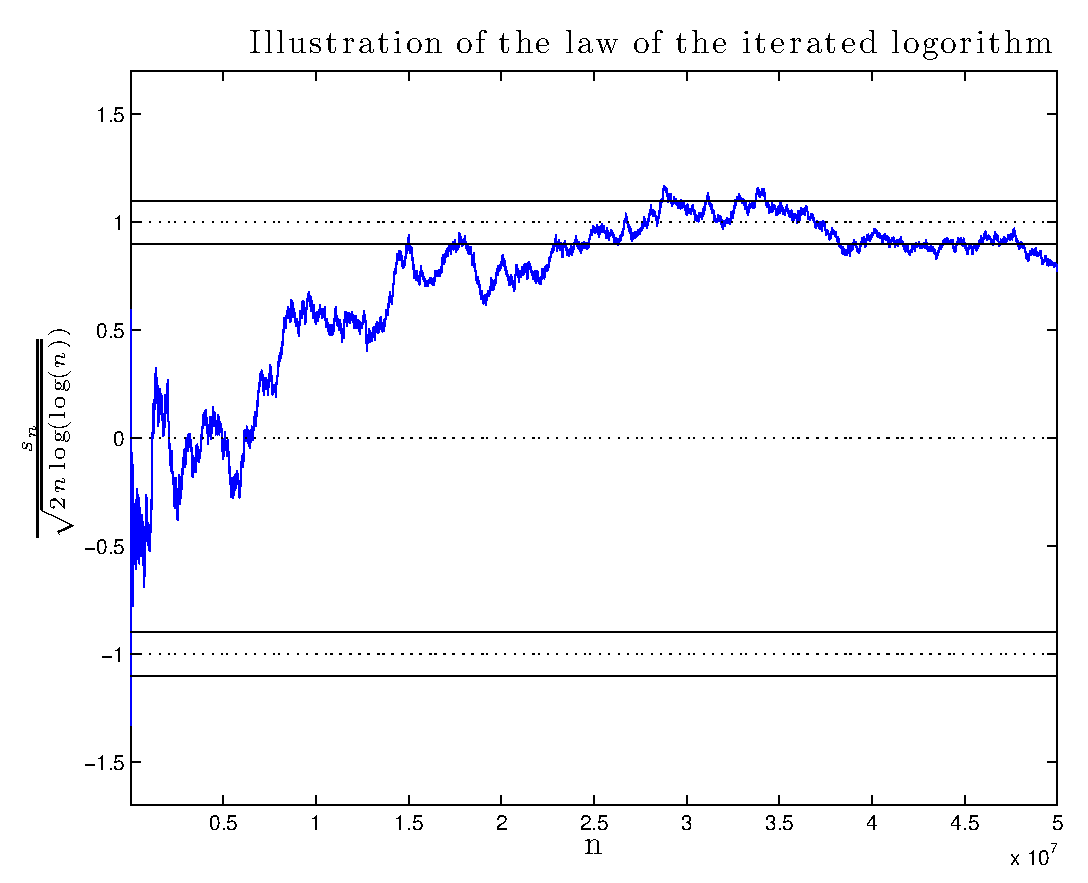
\includegraphics[height = 2.7in]{Measure/LIL.eps}
\end{figure}


\begin{lemma}
\label{LIIL: io lemma 1}
For all $\epsilon > 0 $
\begin{align*}
P[ s_n/\ell_n \geq  (1+\epsilon) \io_n ] = 0
\end{align*}
\end{lemma}
\begin{proof}
The obvious strategy is to use the first Borel-Cantelli lemma. In particular, it would be nice if we could show
\[
\sum_{n=1}^\infty P [ s_n/\ell_n \geq  (1+\epsilon)]<\infty
\]
which would give us the lemma. By the first half of the large deviation result we know $P [ s_n/\ell_n \geq  (1+\epsilon)]$ converge to zero as $n\rightarrow \infty$. Unfortunately, they do not converge fast enough for the first Borel-Cantelli. Taking a sub-sequence will get something summable but we would need to show that the events are well behaved between the sub-sequence. Fortunatly we can do this since the sets $\{s_n/\ell_n \geq  (1+\epsilon)\}$ overlap a lot. The strategy is to group the events $\{s_n/\ell_n \geq  (1+\epsilon)\}$ by unioning them into blocks, then apply Borel-Cantelli on the blocks. This will be sufficient since  the blocks occur infinity often if and only if the events $s_n/\ell_n \geq  (1+\epsilon)$ occur infinity often.  Controlling the probability of the blocks is done with the maximal inequality.

Let the $k^\text{th}$ block be defined
\[
B_k:= \bigcup_{j=n_{k-1}}^{n_k} \{ s_{j}/\ell_{j} \geq  (1+\epsilon) \}
\]
  where $n_k$ is  a (yet to be determined) subsequence. We  use maximal inequality  to bound $P[B_k]$ as follows
\begin{align*}
P[B_k]  &\leq P[\max_{n_{k-1}\leq j\leq n_k} s_j \geq (1+\epsilon)\min_{n_{k-1}\leq j\leq n_k} \ell_{j}] \\
 &\leq P[\max_{n_{k-1}\leq j\leq n_k} s_j \geq (1+\epsilon) \ell_{n_{k-1}}] \\
 &\leq P[\max_{j\leq n_k} s_j \geq (1+\epsilon) \ell_{n_{k-1}}] \\
 &\leq P[\max_{j\leq n_k} s_j \geq \lceil(1+\epsilon) \ell_{n_{k-1}}\rceil],\quad\text{since $s_j\in\Bbb Z$} \\
 &\leq 2P[ s_{n_k} \geq \lceil(1+\epsilon) \ell_{n_{k-1}}\rceil],\quad\text{maximal ineq} \\
 &\leq 2P[ s_{n_k} \geq (1+\epsilon) \ell_{n_{k-1}}] \\
 &\leq \exp\bigl( - \textstyle\frac{1}{2}(1+\epsilon)^2 \ell^2_{n_{k-1}}/n_{k} \bigr),\quad\text{half of large deviation}\\
 &\leq \exp\bigl( - (1+\epsilon)^2 n_{k-1}\log\log n_{k-1}/n_{k} \bigr)\\
 & = \left(\frac{1}{\log n_{k-1}} \right)^{ (1+\epsilon)^2\frac{n_{k-1}}{n_{k}} }.
\end{align*}
Now we just find $n_k$ which makes the last term summable over $k$. If $n_k\approx \theta^k$ one gets
\begin{align*}
\left(\frac{1}{\log n_{k-1}} \right)^{ (1+\epsilon)^2\frac{n_{k-1}}{n_{k}} }
& \approx  \left(\frac{1}{(k-1)\log\theta} \right)^{ (1+\epsilon)^2\frac{1}{\theta} }
\end{align*}
which is summable if $(1+\epsilon)^2\frac{1}{\theta} >1$. We also need that   $\theta > 1$  since we need $n_k\rightarrow \infty$ as $k\rightarrow \infty$. Luckily there does exist such a $\theta$ for which $(1+\epsilon)^2> \theta > 1$.
\end{proof}

\begin{lemma}
\label{LIIL: io lemma 2}
For all $\epsilon >0 $
\begin{align*}
P[ s_n/\ell_n > (1-\epsilon) \io_n ] = 1
\end{align*}
\end{lemma}
\begin{proof}
In the previous lemma we presented a technique to adjust the first Borel-Cantelli lemma in the case the summability condition doesn't hold. For this  lemma we want to use the second Borel-Cantelli lemma but, again, it doesn't directly apply since the condition that the events $s_n/\ell_n > (1-\epsilon)$ are independent does not hold. Here is a generic technique to get around this obstacle. Find subsequence $n_k$ and subsets
\[
I_k \subset   \{s_{n_k}/\ell_{n_k} > (1-\epsilon)\}
\]
such that $I_k$'s  are independent and $\sum_k P[I_k]=\infty$ so that $P[I_k \io_k]=1$ (which would then give the lemma). Unfortunately, even this doesn't work. What ends up working is to find two sets $A_k$ $I_k$ such that
\begin{align}
&A_k\cap I_k \subset \{s_{n_k}/\ell_{n_k} > (1-\epsilon)\}  \label{ABns in wwt}\\
&\text{$I_k$ are independent and $\textstyle\sum_k P[I_k]=\infty$} \label{Bns ind}\\
&\text{$A_k$ are not independent but $P[A_k \aall_k] = 1$.}\label{Ans Borel}
\end{align}
To see why this is sufficient notice that (\ref{Bns ind}) implies $P[I_k \io_k] = 1$ by the second Borel-Cantelli lemma. Then
\begin{align*}
&\text{ $P[A_k \aall_k] = 1$ and $P[I_k \io_k]=1$ } \\
&\qquad\Longrightarrow P[A_k \cap I_k \io_k] = 1 \\
&\qquad\overset{(\ref{ABns in wwt})}\Longrightarrow  P[s_{n_k}/\ell_{n_k} > (1-\epsilon) \io_k] = 1
\end{align*}
Therefore (\ref{ABns in wwt}), (\ref{Bns ind}) and (\ref{Ans Borel}) are sufficient to establish the lemma.

Figuring out how to define $I_k$ and $A_k$ are the tricky parts. The intuition is that if your going to get independent events you need to look at increments of $s_{n}$. Define
\begin{align*}
I_k &:= \{s_{n_k}-s_{n_{k-1}} \geq (1-\epsilon/2)\ell_{n_k}  \} \\
A_k &:= \{ s_{n_{k-1}} > -(\epsilon/2)\ell_{n_k}  \}.
\end{align*}
Clearly  $I_k \cap A_k \subset \{s_{n_k}/\ell_{n_k} > (1-\epsilon)\}$ so that (\ref{ABns in wwt}) holds. Moreover, the $I_k$'s  are independent.
To show (\ref{Ans Borel})
\begin{align*}
P[A_k \aall_k] &= P\Bigl[s_{n_{k-1}} > -(\epsilon/2)\ell_{n_k} \aall_k\Bigr] \\
 &= P\Bigl[s_{n_{k-1}} < (\epsilon/2)\ell_{n_k} \aall_k\Bigr],\quad\text{by symmetry} \\
&= P\Bigl[\frac{s_{n_{k-1}}}{\ell_{n_{k-1}}} < (\epsilon/2)\frac{ \ell_{n_k} }{ \ell_{n_{k-1}} } \aall_k\Bigr] \\
&= 1- P\Bigl[\frac{s_{n_{k-1}}}{\ell_{n_{k-1}}} \geq (\epsilon/2)\frac{ \ell_{n_k} }{ \ell_{n_{k-1}} } \io_k\Bigr] \\
&= 1,\,\text{by Lemma \ref{LIIL: io lemma 1} if \textcolor{blue}{$\frac{\ell_{n_k}}{\ell_{n_{k-1}}}\rightarrow \infty$.}}
\end{align*}
To show (\ref{Bns ind}) notice
\begin{align}
P[I_k] &= P\Bigl[ s_{n_k}-s_{n_{k-1}}\geq(1-\epsilon/2)\ell_{n_k}\Bigr] \nonumber\\
&= P\Bigl[s_{n_k-n_{k-1}}\geq(1-\epsilon/2)\ell_{n_k}\Bigr] \nonumber\\
&\geq P\Bigl[\frac{s_{n_k-n_{k-1}}}{\sqrt{n_k - n_{k-1}}}  \geq \frac{(1-\epsilon/2)\ell_{n_k}}{\sqrt{n_k - n_{k-1}}} \Bigr] \nonumber\\
&\geq \exp\Bigl(-\frac{1}{2}\Bigl[\frac{(1-\epsilon/2)\ell_{n_k}}{\sqrt{n_k - n_{k-1}}}\Bigr]^2(1+o(1))  \Bigr),\label{make this diverge}\\
&\qquad\qquad\text{\textcolor{blue}{by Lemma \ref{LIL: usefull lemma 2} if:}}\nonumber\\
&\qquad\qquad\quad\text{ \textcolor{blue}{$\textstyle\frac{\ell_{n_k}}{\sqrt{n_k - n_{k-1}}}\rightarrow \infty$ and  }}\nonumber\\
&\qquad\qquad\quad\text{ \textcolor{blue}{$\textstyle\frac{1}{\sqrt{n_k - n_{k-1}}}\frac{\ell_{n_k}}{\sqrt{n_k - n_{k-1}}}\rightarrow 0$ and }}\nonumber\\
&\qquad\qquad\quad\text{ \textcolor{blue}{$n_k - n_{k-1}\rightarrow \infty$. }}\nonumber
\end{align}
To finish the proof of (\ref{Ans Borel}) and (\ref{Bns ind}) we need to find $n_k\rightarrow \infty$ such that $\ell_{n_k}$ satisfies the above conditions and the \textcolor{blue}{sum of (\ref{make this diverge}) diverges}.

A subsequence of the form $n_k := \lfloor\exp(k^\theta)\rfloor$ will work. To check the conditions notice

\begin{align*}
\frac{\ell_{n_k}}{\ell_{n_{k-1}}}
& \sim \frac{ \sqrt{2 \exp(k^\theta) \log k^\theta} }{\sqrt{2 \exp((k-1)^\theta) \log (k-1)^\theta}} \\
& =  \exp\Bigl(\frac{k^\theta - (k-1)^\theta}{2}\Bigr) \frac{\log k}{\log (k-1)}  \\
& =  \exp\Bigl(\frac{\theta(k^*)^{\theta-1}}{2}\Bigr) (1 + o(1)),\quad\text{where $k-1\leq k^*\leq k$} \\
& \longrightarrow  \infty, \quad\text{\textcolor{red}{if  $\theta > 1$}.}
\end{align*}
Also
\begin{align*}
n_k - n_{k-1} & \sim  \exp(k^\theta) - \exp((k-1)^\theta) \\
&= \theta (k^*)^{(\theta-1)} \exp((k^*)^\theta) ,\quad\text{where $k-1\leq k^*\leq k$} \\
&\longrightarrow \infty,\quad\text{\textcolor{red}{if $\theta > 0 $.}}
\end{align*}
And therefore
\begin{align*}
\frac{\ell_{n_k}}{\sqrt{n_k - n_{k-1}}}
& \sim \frac{\sqrt{2 \exp(k^\theta) \log k^\theta}}{\sqrt{ \exp(k^\theta) - \exp((k-1)^\theta) }}   \\
&  = \frac{\sqrt{2\theta\log k}}{\sqrt{ 1 - \exp((k-1)^\theta-k^\theta)  }}  \\
& = \frac{\sqrt{2\theta\log k}}{\sqrt{ 1 - o(1)  }}\\
& \longrightarrow \infty.
\end{align*}
Clearly we now have that  $\frac{\ell_{n_k}}{{n_k - n_{k-1}}}  \longrightarrow 0.$
Finally we need to show that the sum of (\ref{make this diverge}) over $k$ diverges.  The individual terms are
\begin{align*}
\exp\Bigl(-\frac{1}{2}\Bigl[&\frac{(1-\epsilon/2)\ell_{n_k}}{\sqrt{n_k - n_{k-1}}}\Bigr]^2(1+o(1))  \Bigr) \\
& \sim \exp\Bigl(-\frac{(1-\epsilon/2)^2}{2}2\theta \log k   \Bigr) \\
& = \exp\Bigl(-{(1-\epsilon/2)^2}\theta \log k   \Bigr) \\
& = k ^ {-{(1-\epsilon/2)^2}\theta}
\end{align*}
the sum of the above terms over $k$ diverges if $(1-\epsilon/2)^\theta  < 1$, i.e. \textcolor{red}{ if $\theta < \frac{1}{(1-\epsilon)^2}$}. Now putting all the  conditions on $\theta$ together says that we simply need to choose $\theta$ such that
\[ 1<\theta <\frac{1}{(1-\epsilon/2)^2} .\]
\end{proof}



\clearpage
%-------------------------------'
%---------section  ---------------'
%-------------------------------'
\section{Measures}
%-------------------------------'
%---------section  ---------------'
%-------------------------------'

\subsection{Basic theory}





\begin{definition}[{\bf Measure}]
If $\mathcal F_0$ is a field of $\Omega$-sets, then $\mu:\mathcal F_0\rightarrow [0,\infty]$ is a {measure} if
\begin{enumerate}
\item $\mu(\varnothing)=0$
\item $\mu\bigl( \bigcup_{k=1}^\infty A_k \bigr)=\sum_{k=1}^\infty \mu(A_k)$ \\ for all disjoint $A_1, A_2,\ldots \in\mathcal F_0$ such that $\bigcup_{k=1}^\infty A_k \in \mathcal F_0$.
\end{enumerate}
\end{definition}


\begin{definition}[{\bf Measurable space}]
If $\mathcal F$ is a $\sigma$-field on $\Omega$ then the pair $(\Omega, \mathcal F)$  is called a {measurable space}.
\end{definition}


\begin{definition}[{\bf Measure space}]
If $\mu$ is a measure on the measurable space $(\Omega, \mathcal F)$ then the triple $(\Omega, \mathcal F, \mu)$ is called a {measure space}.
%If, in addition, $\mu$ is a probability measure then the triple $(\Omega, \mathcal F, \mu)$ is called a {probability space}.
\end{definition}



\begin{definition}[{\bf Finite and $\sigma$-finite}]
Let $(\Omega, \mathcal F,\mu)$ be a measure space.
\begin{itemize}
\item If $\mu(\Omega)<\infty$ then $\mu$ is said to be a {finite} measure;
\item If $\mu(\Omega)=\infty$ then $\mu$ is said to be an {infinite} measure;
\item If there exists $\mathcal F$-sets $A_1,A_2,\ldots$ such that $\Omega = \cup_{k=1}^\infty A_k$ and $\mu(A_k)<\infty$ then $\mu$ is said to be a {$\sigma$-finite} measure;
\item If $\mathscr A\subset \mathcal F$ such that there exists $\mathscr A$-sets $A_1,A_2,\ldots$ such that $\Omega = \cup_{k=1}^\infty A_k$ and $\mu(A_k)<\infty$ then $\mu$ is said to be {$\sigma$-finite on $\mathscr A$}.
\end{itemize}
\end{definition}

\begin{theorem}[{\bf Basic measure facts}]
Let $(\Omega, \mathcal F, \mu)$ be a measure space. Then
\begin{enumerate}
\item If $A_1, A_2,\ldots, A_n$ are disjoint $\mathcal F$-sets then \\$\mu\bigl(\sum_{k=1}^n A_k\bigr) = \sum_{k=1}^n \mu(A_k)$.
\item If $A\subset B$ are $\mathcal F$-sets then \\$\mu(A)\leq \mu(B)$.
\item If $A\subset B$ are $\mathcal F$-sets and {$\mu(A)<\infty$} then \\$\mu(B-A)=\mu(B)-\mu(A)$.
\item If $A_1, A_2,\ldots $ are $\mathcal F$-sets then \\$\mu\bigl(\sum_{k=1}^\infty A_k\bigr) \leq \sum_{k=1}^\infty \mu(A_k)$.
\item If  $A_1, A_2,\ldots $ are $\mathcal F$-sets such that $A_n\uparrow A$ then \\$\mu(A_n)\uparrow \mu(A)$.
\item If  $A_1, A_2,\ldots $ are $\mathcal F$-sets such that $A_n\downarrow A$ and {$\mu(A_k)<\infty$} for some $k$ then $\mu(A_n)\downarrow \mu(A)$.
\end{enumerate}
\end{theorem}


%%%%%%%%%%%%%%%%%
\begin{theorem}[{\bf Uniqueness for measures}]
\label{uui}
If $\mu_1$ and $\mu_2$ are measures on $(\Omega, \sigma\langle \mathcal P\rangle)$ such that
\begin{enumerate}
\item $\mu_1$ and $\mu_2$ agree on $\mathcal P$;
\item $\mathcal P$ is a $\pi$-system;
\item $\mu_1$ and $\mu_2$ are $\sigma$-finite on $\mathcal P$,
\end{enumerate}
then $\mu_1$ and $\mu_2$ agree on all of $ \sigma\langle \mathcal P\rangle$.
\end{theorem}




\begin{definition}[{\bf $\mu$-null and $\mu$-neg}]
%$\phantom{asdf}$
Let $(\Omega,\mathcal F, \mu)$ be a measure space. Then
%then
\begin{itemize}
\item
A set $A\in \mathcal F$ is said to be {$\mu$-null}  if $\mu(A)=0$.
\item
A set $A\in 2^\Omega$ is said to be {$\mu$-negligible} if there exists a $\mu$-null set  $B\in \mathcal F$ such that $A\subset B$.
\end{itemize}
\end{definition}



\begin{definition}[{\bf Complete}]
A measure space $(\Omega^\prime, \mathcal F^\prime, \mu^\prime)$ is said to be complete if all the $\mu^\prime$-negligible sets belong to $\mathcal F^\prime$.
\end{definition}

\begin{theorem}[{\bf The completion $(\Omega, \bar {\mathcal F},\bar \mu)$}]
Let $(\Omega,\mathcal F, \mu)$ be a measure space and let $\mathcal N_\mu$ be the collection of $\mu$-negligible sets.
%Let $\bar {\mathcal F}:=\sigma\langle \mathcal F, \mathcal N_\mu\rangle$ and $\bar \mu$
Then
\begin{itemize}
\item $\bar {\mathcal F}:= \sigma\langle \mathcal F, \mathcal N_\mu\rangle = \{F\cup N: F\in \mathcal F, N\in \mathcal N_\mu  \}$;
\item The set function $\bar \mu$ on $\bar{\mathcal F}$ defined by $\bar\mu(F\cup N)= \mu(F)$ for $F\in\mathcal F$ and $N\in \mathcal N_\mu$ is the unique extension of $\mu$ to a measure on $(\Omega, \bar{\mathcal F})$;
\item The measure space $(\Omega, \bar{\mathcal F}, \bar \mu)$ is complete.
\end{itemize}
The triple $(\Omega, \bar{\mathcal F}, \bar \mu)$ is called the {completion} of  $(\Omega, \mathcal F, \mu)$.
\end{theorem}









%%%%%%%%
\begin{exercise}
\label{l1}
Suppose  $\mathcal F_0$ is a field, $\mu$ is a measure on $\sigma\langle \mathcal F_0\rangle$ and $\mu$ is $\sigma$-finite on $\mathcal F_0$.
\begin{enumerate}
\item
Suppose $B\in \sigma\langle\mathcal F_0\rangle$ and $\epsilon>0$. Show that there exists a disjoint sequence of $\mathcal F_0$-sets $A_1, A_2,\ldots$ such that $B\subset \cup_{n=1}^\infty A_n$ and $ \mu\bigl( \cup_{n=1}^\infty A_n -
 B\bigr)\leq \epsilon$.
 \item Suppose $B\in \sigma\langle\mathcal F_0\rangle$, $\mu(B)<\infty$ and $\epsilon>0$. Show there exists an $\mathcal F_0$-set $A$ such that $\mu(A \,\triangle\, B)\leq \epsilon$.
\item Show by example that the conclusion to 2 may fail if $B$ has infinite measure.
 \end{enumerate}
\end{exercise}


\begin{exerciseproof}

\textbullet({\sl Show 1:})
Since $\mu$ is $\sigma$-finite on $\mathcal F_0$ and $\mathcal F_0$ is a field, one can find disjoint $\mathcal F_0$-sets $F_1, F_2,\ldots$ such that $\Omega = \cup_{n=1}^\infty F_n$ and $\mu(F_n)<\infty$. We start by supposing $\mu(F_n)>0$ for all $n$ and show at the end of the proof to remove this assumption.


Fix $B\in \mathcal F$.
Define  $ \mu_n(\cdot):= \frac{\mu(\cdot\cap F_n)}{\mu(F_n)} $ on $\mathcal F$. Notice that $\mu_n$ is a probability measure on $\mathcal F$ so that
\[ \mu_n(B)=\inf\{ \mu_n(D): B\subset D \in \mathcal F^{\uparrow}\}\leq 1. \]
Therefore one can find a $D_n\in \mathcal F^{\uparrow}$, covering $B$, such that
$B\subset D_n$ and
\begin{align}
\label{aaa}
\underbrace{\mu_n(D_n)-\mu_n(B)}_{=\mu_n(D_n - B)} &\leq \frac{\epsilon}{2^n \mu(F_n)}.
\end{align}
 Now define  $D :=\bigcup_{n=1}^\infty D_n\cap F_n$
and notice that
\begin{align*}
 B\subset D_n, \,\forall n&\Rightarrow (B\cap F_n) \subset (D_n\cap F_n), \,\forall n \\
 &\Rightarrow \bigcup_{n=1}^\infty  (B\cap  F_n) \subset  \bigcup_{n=1}^\infty (D_n\cap F_n) \\
 &\Rightarrow B\subset D.
 \end{align*}
Notice also that each  $D_n\in\mathcal F^\uparrow$ can be written as a disjoint union of $\mathcal F_0$-sets (exercise). Let $D_n = \cup_{m=1}^\infty A_{n,m}$ be such a decomposition (i.e. the $A_{n,m}$'s are  disjoint across $m$ and $A_{n,m}\in\mathcal F_0$). Then
\[D =  \bigcup_{(n,m)\in \Bbb N^+\times \Bbb N^+}  A_{n,m}\cap F_n\]
where the sets $A_{n,m}\cap F_n$ are disjoint (the $F_n$'s are disjoint for different $n$'s and  the $A_{n,m}$'s are disjoint for different $m$'s) and are $\mathcal F_0$-sets. Now
\begin{align}
\mu(D - B) &= \mu(\bigcup_{n=1}^\infty D_n\cap F_n \cap B^c)\nonumber\\
 &= \sum_{n=1}^\infty \mu(D_n\cap F_n \cap B^c)\nonumber\\
 &=  \sum_{n=1}^\infty \mu(F_n)\mu_n(D_n \cap B^c)\nonumber\\
  &=  \sum_{n=1}^\infty \mu(F_n)\underbrace{\mu_n(D_n - B)}_{\leq \epsilon/(2^n\mu(F_n))}\nonumber\\
 &\leq \epsilon.\label{if}
\end{align}
Therefore the class $\{ A_{n,m}\cap F_n\}_{(n,m)\in \Bbb N^+\times \Bbb N^+ }$ gives a countable, disjoint $\mathcal F_0$-set covering of $B$ such that $\mu(\bigcup_{(n,m)\in \Bbb N^+\times \Bbb N^+}  A_{n,m}\cap F_n - B )\leq \epsilon$.

It's easy to extend to the case when some of the $\mu(F_n)=0$ by defining $\mu_n (\cdot):=0$ and $D_n:=F_n$ for these $n$. Then (\ref{if}) still follows.

\textbullet({\sl Show 2:})
Since $\mu(B)<\infty$ we have that
\begin{equation}
 \mu(D)-\mu(B)=\mu(D-B)\leq \epsilon.
\end{equation}
Therefore $\mu(D)<\infty$
Moreover $D=\setlimup{n}D_n$, where $D_n\in \mathcal F_0$ are the $n$ partial unions in the defintion of $D$.
Therefore $\mu(D_n)\uparrow \mu(D)<\infty$ and hence we can fine a
 a $D_n$ such that $D_n\subset D$ and
\begin{equation}
\mu(D) - \mu(D_n)=\mu(D - D_n)\leq \epsilon
\end{equation}
Now
\begin{align*}
\mu(B\,\triangle\, D_n)
&\leq \mu(B\cap D_n^c) + \mu(B^c \cap D_n)\\
&\leq \mu(D \cap D_n^c) + \mu(B^c \cap D)\\
&= \mu(D - D_n) + \mu(D - A)\\
&\leq 2\epsilon.
\end{align*}
\end{exerciseproof}






\begin{exercise}
Suppose that $\mu_1$ and $\mu_2$ are measures on  $\sigma\langle \mathcal F_0\rangle$ generated by a class $\mathcal F_0$. Suppose also that the inequality
\begin{equation}
\label{fourteen}
\mu_1(A)\leq \mu_2(A)
\end{equation}
holds for all $A$ in $\mathcal F_0$. (a) Show that if $\mathcal F_0$ is a field and $\mu_1$ and $\mu_2$ are $\sigma$-finite on $\mathcal F_0$, then (\ref{fourteen}) holds for all $A\in\sigma\langle \mathcal F_0\rangle$. (b) Show by examples that (\ref{fourteen}) can fail for some $A\in\sigma\langle \mathcal F_0\rangle$ if: $\mathcal F_0$ is a field but $\mu_1$ and $\mu_2$ are only $\sigma$-finite  overall, not $\sigma$-finite on $\mathcal F_0$; or if $\mu_1$ and $\mu_2$ are $\sigma$-finite on $\mathcal F_0$, but $\mathcal F_0$ is only a $\pi$-system. Hint: for (a) first treat the case where $\mu_2$ is finite.
\end{exercise}



%-------------------------------'
%---------section  ---------------'
%-------------------------------'
\subsection{Lebesque Measure}
%-------------------------------'
%---------section  ---------------'
%-------------------------------'



For any $\bs i=(i_1,\ldots, i_d)\in\Bbb Z^d$ let $(\bs i,\bs i+1]$ be the unit cube in $\Bbb R^d$ translated up by $\bs i$ so that
\[(\bs i,\bs i+1] \equiv (i_1, i_1+1]\times \cdots \times (i_d,i_d + 1].  \]
Notice that these sets give a checker board decomposition, $\Bbb R^d=\bigcup_{\bs i\in\Bbb Z^d} (\bs i,\bs i+1] $, so that $\Bbb R^d$ is expressed as a countable disjoint union of the translated unit cubes. Let $\mathcal B_{0}^{(\bs i,\bs i+1] }$ denote the field of finite disjoint unions of rectangles in $(\bs i,\bs i+1] $ and let $\mathcal B^{(\bs i,\bs i+1] }\equiv \sigma \langle \mathcal B_{0}^{(\bs i,\bs i+1] }\rangle $ denote the Borel $\sigma$-field of  $(\bs i,\bs i+1]$. Finally let $P_{\bs i}$ denote the unique uniform probability measure on $\mathcal B^{(\bs i,\bs i+1] }$ which assigns Euclidean volume  to the rectangles in  $(\bs i,\bs i+1] $, i.e.
\[ P_{\bs i}\bigl( (a_1,b_1]\times \cdots \times (a_d,b_d]\bigr)=\prod_{k=1}^d (b_k - a_k) \]
whenever $(a_1,b_1]\times \cdots \times (a_d,b_d]\subset (\bs i,\bs i+1]$. The construction of $P_{\bs i}$ is done in exactly the same way as the uniform probability measure was constructed on $(0,1]$ in the beginning of the class. Lets recall how this is done. One first shows that for any $A\in \mathcal \mathcal B_{0}^{(\bs i,\bs i+1] }$ one can define $P_{\bs i}(A)$ to be the sum  of the disjoint rectangle volumes which make up $A$ (this is not trivial since there are different decompositions of $A$ into disjoint rectangles, but one can use a result similar to Theorem 1.3 of Billingsley to prove that $P_{\bs i}$ is well defined).  Secondly, one shows that $P_{\bs i}$ is a probability measure on $((\bs i, \bs i +1],\mathcal B_{0}^{(\bs i,\bs i+1] })$. The hard part of this step is to  show the countable additivity. For $(0,1]$ we used the equivalent condition that  $P_{\bs i}$ is continuous from above at $\varnothing$. This argument carries over to $((\bs i, \bs i +1],\mathcal B_{0}^{(\bs i,\bs i+1] }, P_{\bs i})$. Finally one invokes the Carath\'eodory Extension theorem to get a uniform probability measure $((\bs i, \bs i +1],\mathcal B^{(\bs i,\bs i+1] }, P_{\bs i})$ (uniqueness follows by the fact that rectangles, including the empty ones, form a $\pi$-system).

Now, using the uniform probability measures $((\bs i, \bs i +1],\mathcal B^{(\bs i,\bs i+1] }, P_{\bs i})$ we can define Lebesque measure $\mathcal L^d$ on sets $A\in\mathcal B^{(\bs i,\bs i+1] }$ by stitching these $P_{\bs i}$ together as follows
\begin{equation}
\label{Lm}
 \mathcal L^d(A):= \sum_{\bs i\in\Bbb Z^d} P_{\bs i}\bigl( (\bs i, \bs i+1]\cap A\bigr).
 \end{equation}
Notice that each $ (\bs i, \bs i+1]\cap A$ is in the Borel $\sigma$-field $\mathcal B^{(\bs i,\bs i+1] }$ by Claim \ref{restricTHM} so that
$P_{\bs i}\bigl( (\bs i, \bs i+1]\cap A\bigr)$ is defined.
Lets see that $\mathcal L^d$ is indeed a measure on $(\Bbb R^d,\mathcal B^{\Bbb R^d })$.


\begin{theorem}
 $\mathcal L^d$  is a measure on $(\Bbb R^d,\mathcal B^{\Bbb R^d })$.
\end{theorem}
\begin{proof}
We show the following three axioms (i), (ii) and (iii):
\begin{enumerate}
\item[(i)] $\mathcal L^d(A)\in [0,\infty]$: Trivial.
 \item[(ii)]  $\mathcal L^d(\varnothing)=0$: This is also easy since $P_{\bs i}\bigl( (\bs i, \bs i+1]\cap \varnothing\bigr)=0$.
\item[(iii)] Countable additivity: Suppose $A_1,A_2,\ldots\in\mathcal B^{\Bbb R^d }$ are disjoint. Then
\begin{align}
\mathcal L^d\Bigl (\bigcup_{k=1}^\infty A_k\Bigr)&=\sum_{\bs i\in\Bbb Z^d} P_{\bs i}\Bigl((\bs i, \bs i+1] \cap \bigcup_{k=1}^\infty A_k \Bigr) \nonumber\\
&=\sum_{\bs i\in\Bbb Z^d} P_{\bs i}\Bigl( \bigcup_{k=1}^\infty (\bs i, \bs i+1] \cap A_k \Bigr) \nonumber\\
&=\sum_{\bs i\in\Bbb Z^d} \sum_{k=1}^\infty P_{\bs i} \Bigl((\bs i, \bs i+1] \cap A_k \Bigr)\label{se} \\
&=\sum_{k=1}^\infty  \sum_{\bs i\in\Bbb Z^d} P_{\bs i} \Bigl((\bs i, \bs i+1] \cap A_k \Bigr)\label{se2} \\
&=\sum_{k=1}^\infty  \mathcal L^d\bigl (A_k \bigr) \nonumber
\end{align}
where (\ref{se}) follows since $P_{\bs i}$ is countably additive and the $ (\bs i, \bs i+1]\cap A_k $'s are disjoint; and (\ref{se2}) follows from general results about positive iterated sums.
\end{enumerate}
\end{proof}



 \begin{theorem}
 \label{ui2}
  $\mathcal L^d$ is the only measure on $(\Bbb R^d,\mathcal B^{(0,1]^d})$ which assigns standard Euclidean volume to the finite rectangles as follows
 \begin{equation}
\mathcal L^d \bigl( (a_1,b_1]\times \cdots \times (a_d,b_d]\bigr)=\prod_{k=1}^d (b_k - a_k)
\end{equation}
for $-\infty < a_k < b_k <\infty$.
\end{theorem}
\begin{proof}
Define $\mathcal P$ to be the $\pi$-system composed of the finite rectangles $\{ (a_1,b_1]\times \cdots \times (a_d,b_d]: -\infty < a_k < b_k <\infty\}$ and the empty set $\varnothing$. One can easily establish that $\mathcal B^{\Bbb R^d}=\sigma\langle\mathcal P\rangle$.
 Also notice that $\mathcal L^d$ is $\sigma$-finite on $\mathcal P$ since  $\mathcal L^d\bigl((\bs i,\bs i+1])=1$, $\Bbb R^d = \cup_{\bs i\in\Bbb Z^d} (\bs i,\bs i+1]$ and each $(\bs i,\bs i+1]\in \mathcal P$.
 Therefore Theorem \ref{uui} establishes the following claim
\end{proof}




\begin{theorem}
For any $A\in\mathcal  B^{\Bbb R^d}$ and $x\in \Bbb R^d$, the set $A+x:= \{ a+x: a\in A\}$ is in $\mathcal B^{\Bbb R^d }$ and
\begin{equation}
 \label{translate}
 \mathcal L^d(A+x) =  \mathcal L^d(A)
 \end{equation}
\end{theorem}
\begin{proof}
To show $A+x \in\mathcal B^{\Bbb R^d }$ use the good sets principle. Fix $x\in \Bbb R^d$ and set   $\mathcal G_x:=\{ A\in \mathcal B^{\Bbb R^d }:  A+x \in \mathcal B^{\Bbb R^d }\}$.
It is easy to see that $\mathcal G_x$ is a $\sigma$-field since complementation and union is preserved under translation by $x$. For example,
\begin{align*}
A\in\mathcal G_x &\Rightarrow  A\in \mathcal B^{\Bbb R^d } \text{  and } A+x \in \mathcal B^{\Bbb R^d } \\
&\Rightarrow  A^c\in \mathcal B^{\Bbb R^d } \text{  and } (A+x)^c \in \mathcal B^{\Bbb R^d } \\
&\Rightarrow  A^c\in \mathcal B^{\Bbb R^d } \text{  and } A^c+x \in \mathcal B^{\Bbb R^d } \\
&\Rightarrow A^c\in\mathcal G_x.
\end{align*}
The other axioms are established in a similar fashion.
Moreover, clearly all the finite rectangles are in $\mathcal G_x$. Therefore good sets implies $\mathcal B^{\Bbb R^d } \subset \mathcal G_x$  which implies $A\in \mathcal B^{\Bbb R^d }\rightarrow A+x \in \mathcal B^{\Bbb R^d }$, as was to be shown.

Now to show (\ref{translate}) one can simply use the same arguments used in the Theorem \ref{ui2} on the uniqueness of $\mathcal L^d$. In particular, fix $x$ and define $\mu_x(A):= \mathcal L^d(A+x)$. It is easy to show that $\mu_x$ is a measure on $(\Bbb R^d, \mathcal B^{\Bbb R^d })$. Moreover, since the volume of any rectangle in $\Bbb R^d$ is invariant under translation by $x$, the measures $\mu_x$ and $\mathcal L^d$ both agree on the $\pi$-system of finite, possibly empty, rectangles in $\Bbb R^d$. Since they are also both $\sigma$-finite on these rectangles one must have, by Theorem \ref{ui2}, $\mathcal L^d(A) =\mu_x(A):= \mathcal L^d(A+x) $ for all $A\in\mathcal B^{\Bbb R^d }$, as was to be shown.
\end{proof}

%%%%%%%%%%%%%%%
\begin{theorem}
If $T:\Bbb R^d\rightarrow \Bbb R^d$ is linear and nonsingular, then $A\in\mathcal B^{\Bbb R^d}$ implies that $T\!A:=\{ T(a): a\in A\}\in \mathcal B^{\Bbb R^d}$ and
\[ \mathcal L^d(T\!A):=|\det T |\mathcal L^d(A). \]
\end{theorem}

%%
\begin{theorem}
\label{cc}
Let $(\Omega, \mathcal F,\mu)$ be a $\sigma$-finite measure space. Then $\mathcal F$ cannot contain an uncountable, disjoint collection of sets of positive $\mu$-measure
\end{theorem}
\begin{proof}
Let $\{B_i: i\in \mathcal I\}$ a disjoint collection of sets of such that $\mu(B_i)>0$ for each $i\in\mathcal I$.
We show $\mathcal I$ must be countable.


Since $\mu$ is $\sigma$-finite there exists $A_1,A_2,\ldots \in\mathcal F$ such that $\mu(A_k)<\infty$ and $\Omega = \cup_k A_k$.  We show the following three facts.
\begin{itemize}
\item $\{ i\in \mathcal I: \mu(A_k\cap B_i)>\epsilon\}$ is finite for all $k$:
Let $\epsilon>0$ and suppose by contradiction one can find a countably infinite set  $\mathcal I_c\subset \mathcal I$ such that $\mu(A_k\cap B_i)>\epsilon $ for all $i\in \mathcal I_c$ and for this set of indices one has
\begin{align*}
\mu(A_k)&\geq \mu(A_k\cap (\cup_{i\in\mathcal I_c}B_i ))= \sum_{i\in\mathcal I_c}\mu(A_k\cap B_i) > \sum_{i\in\mathcal I_c}\epsilon =\infty
\end{align*}
which gives a contradiction.
\item $\{ i\in \mathcal I: \mu(A_k\cap B_i)>0\}$ is countable for all $k$:
This follows from the  identity
\[\{ i\in \mathcal I: \mu(A_k\cap B_i)>0\}=\bigcup_\text{\small rational
$\epsilon$} \underbrace{\{ i\in \mathcal I: \mu(A\cap B_i)>\epsilon\}.} _\text{\small finite by (i)}   \]
\item $\mathcal I = \bigcup_k \{ i\in \mathcal I: \mu(A_k\cap B_i)>0\}$:
 To show $\mathcal I \cup \bigcup_k \{ i\in \mathcal I: \mu(A_k\cap B_i)>0\}$ notice that  if $i\in\mathcal I$ then $\mu(B_i)>0$. Now  $\Omega =\cup_k A_k$ so there must exist a $k$ such that $\mu(A_k\cap B_i)>0$.  Therefore $i\in  \bigcup_k \{ i\in \mathcal I: \mu(A_k\cap B_i)>0\}$. The other inclusion is obvious.
\end{itemize}

 To finish the proof simply notice that the last two bullets imply $\mathcal I$ is countable.
\end{proof}


%%%%%%%
\begin{corollary}If $k<d$ then
$\mathcal L^d(A)=0$ for any $k$-dimensional hyperplane $A\subset \Bbb R^d$ where $k<d$.
\end{corollary}
\begin{proof}
Let $A$ be a $k$-dimensional hyperplane where $k<d$. Let $x$ be a point in $\Bbb R^d$ which is not  contained in $A$.
Then $\{A+xt: t\in\Bbb R\}$ is an uncountable class of disjoint subsets of $\mathcal B^{\Bbb R^d}$. Since $\mathcal L^d$ is translation invariance $\mathcal L^d(A) = \mathcal L^d(A+xt)$ for each $t\in\Bbb R$. Now by Theorem \ref{cc}, $\mathcal L^d(A)=0$, for otherwise there would exists a uncountable, disjoint collection of sets of positive $\mathcal L^d$-measure.
\end{proof}





%%%%%%%%%%%%%%
\begin{theorem}[{\bf Regularity}]
\label{oir}
Let $\mu$ be any measure on $(\Bbb R^d,\mathcal B^{\Bbb R^d})$ which assigns finite measure to bounded sets in $\mathcal B^{\Bbb R^d}$.
For any  $B\in\mathcal B^{\Bbb R^d}$ and $\epsilon>0$ there exists a closed set $C$ and an open set $O$ such that $C\subset B\subset O$ and
\[\mathcal \mu(O-C)<\epsilon.\]
\end{theorem}

%%%%%%%%%%%%%%%%%%%%%%%%
\begin{corollary}
\label{ir}
Let $\mu$ be any measure on $(\Bbb R^d,\mathcal B^{\Bbb R^d})$ which assigns finite measure to bounded sets in $\mathcal B^{\Bbb R^d}$. Then
\begin{align*}
\mathcal \mu(B)  &= \sup \{ \mathcal \mu(C):  C\subset B,\, \text{$C$ closed}\}\\
  &=\, \inf \{ \mu(O):  B\subset O,\, \text{$O$ open}\}
\end{align*}
%If, in addition,  $\mathcal \mu(B)<\infty$ then
%\[\mathcal \mu(B) = \sup \{ \mathcal \mu(K):  K\subset B,\, \text{$K$ compact}\} .\]
\end{corollary}


\begin{definition}[{\bf Borel versus Lebesque measurable sets}]
Let $\bigl(\Omega,\overline{\mathcal B^{\Bbb R^d}},\overline{\mathcal L^d}\bigr)$ be the completion of $(\Omega, \mathcal B^{\Bbb R^d},\mathcal L^d)$. If $A\in \mathcal B^{\Bbb R^d}$ then $A$ is said to be {Borel measurable}. If $A\in \overline{\mathcal B^{\Bbb R^d}}$ then $A$ is said to be {Lebesque measurable}.
\end{definition}

\begin{theorem}[{\bf This is why we need $\sigma$-fields}]
$\phantom{asdf}$
\begin{itemize}
\item $\mathcal B^{\Bbb R}\subsetneq \overline{\mathcal B^{\Bbb R}} \subsetneq 2^\Bbb R$.
\item It is impossible to put a measure on $2^\Bbb R$ which is translation invariant and which assigns normal length to finite intervals. Put another way---there is no Lebesque measure on all of $2^\Bbb R$. Or another way---it is impossible to consistently assign a length to all subsets of $\Bbb R$.
\end{itemize}
\end{theorem}





\begin{exercise}
Prove Theorem \ref{oir} for $d=1$
\end{exercise}




\begin{exercise}
(a) Prove Corollary \ref{ir} for $d=1$.
(b)
Give an example of a $\sigma$-finite measure $\mu$ on $\mathcal B^{\Bbb R}$ and a Borel set $B$ such that
\[ \mu(B-C)= \infty = \mu(O-B) \]
for every closed subset $C$ of $B$ and every open superset $O$ of $B$.
\end{exercise}


\clearpage
%-------------------------------'
%---------section  ---------------'
%-------------------------------'
\section{Measurable functions}
%-------------------------------'
%---------section  ---------------'
%-------------------------------'

\subsection{Basic theory}

\begin{definition}[{\bf Measurable functions}]
If $(\Omega_1, \mathcal F_1)$ and $(\Omega_2,\mathcal F_2)$ are measurable spaces then $f\colon \Omega_1 \rightarrow \Omega_2$ is said to be {measurable between $\mathcal F_1$ and $\mathcal F_2$} (written $f\mcirc \mathcal F_1/\mathcal F_2$) if and only if
\[ f^{-1}(A)\in \mathcal F_1,\quad\forall A\in\mathcal F_2\]
where $ f^{-1}(A):=\{w\in\Omega_1: f(w)\in A \}$.
\end{definition}


\begin{theorem}[{\bf Basic facts about pull backs}]
\label{thm pull back basic facts}
Let $f\colon \Omega_1 \rightarrow \Omega_2$. Let $A, A_1, A_2, \ldots \subset \Omega_2$. Then
\begin{itemize}
\item $f^{-1}(\Omega_2) = \Omega_1$
\item $f^{-1}(\varnothing) = \varnothing$
\item $f^{-1}(\Omega_2 - A) = \Omega_1 - f^{-1}(A)$
\item $f^{-1}(\cup_i A_i) =  \cup_i  f^{-1}(A_i)$
\item $f^{-1}(\cap_i A_i) = \cap_i  f^{-1}(A_i)$.
\end{itemize}
\end{theorem}
\begin{proof} These are very easy to check. For example  to see why $f^{-1}(\cup_i A_i) \subset  \cup_i  f^{-1}(A_i)$ notice that
\begin{align*}
\omega \in f^{-1}(\cup_i A_i)
&\Longrightarrow f(\omega) \in \cup_i A_i \\
&\Longrightarrow \text{$f(\omega) \in A_i$ for some $i$ }\\
&\Longrightarrow \text{$\omega \in f^{-1}(A_i)$ for some $i$ }\\
&\Longrightarrow \omega \in \cup_i f^{-1}(A_i).
\end{align*}
The other arguments are exactly similar.
\end{proof}


\begin{theorem}[{\bf Generators are enough}]
\label{thm: GaE}
Let $(\Omega_1, \mathcal F_1)$ and $(\Omega_2,\mathcal F_2)$ be  measurable spaces where $\mathcal F_2$ is generated by some class $\mathcal A\subset 2^{\Omega_2}$ (i.e. $\mathcal F_2=\sigma\langle \mathcal A\rangle$). If $f:\Omega_1\rightarrow \Omega_2$ then
\[ f \mcirc \mathcal F_1/\mathcal F_2 \Longleftrightarrow f^{-1}(A)\in\mathcal F_1,\,\, \forall A\in\mathcal A.\]
\end{theorem}



\begin{corollary}[{\bf Monotone real maps are measurable}]
Any monotone map $f\colon \Bbb R\rightarrow \Bbb R$ is measurable $\mathcal B^{\Bbb R}/\mathcal B^{\Bbb R}$.
\end{corollary}

\begin{corollary}[{\bf Continuous real maps are measurable}]
Any continuous map $f\colon \Bbb R^d\rightarrow \Bbb R^k$ is measurable $\mathcal B^{\Bbb R^d}/\mathcal B^{\Bbb R^k}$.
\end{corollary}




\begin{theorem}[{\bf Composition of $\mcirc$ functions is $\mcirc$}]
\label{thm: composition of measurable}
Let $(\Omega_1,\mathcal F_1)$, $(\Omega_2,\mathcal F_2)$ and $(\Omega_3,\mathcal F_3)$ be measurable spaces. Suppose $f$ and $g$ are functions sending $\Omega_1\overset{f} \longmapsto \Omega_2 \overset{g}\longmapsto \Omega_3$. If $f\mcirc \mathcal F_1/\mathcal F_2$ and $g\mcirc  \mathcal F_2/\mathcal F_3$ then $g\circ f \mcirc\mathcal F_1/\mathcal F_3$.
\end{theorem}


\begin{corollary}[{\bf Just check that each coordinate is $\mcirc$}]
\label{coordM}
Let $(\Omega,\mathcal F)$ be a measurable space and $f:\Omega\rightarrow \Bbb R^d$. Let $f=(f_1,\ldots, f_d)$ decompose $f$ into the coordinate functions (so that $f_k:\Omega\rightarrow \Bbb R$). Then
\[ f\mcirc \mathcal F/\mathcal B^{\Bbb R^d}\Longleftrightarrow  f_k\mcirc \mathcal F/\mathcal B^{\Bbb R}, \text{ for each $k$.} \]
\end{corollary}



\begin{theorem}[{\bf Scissors and paste}]
Let $(\Omega_1, \mathcal F_1)$ and $(\Omega_2,\mathcal F_2)$ be measurable spaces and $f\colon \Omega_1 \rightarrow \Omega_2$.  In addition, suppose there exists $\mathcal F_1$-sets $A_1,A_2,\ldots$ such that $\Omega_1 = \cup_{k=1}^\infty A_k$. Then
\[ f\mcirc \mathcal F_1/\mathcal F_2 \Longleftrightarrow  f\bigr|_{A_k} \mcirc (\mathcal F_1\!\cap\! A_k)/\mathcal F_2, \text{ for each $k$.} \]
\end{theorem}

\begin{corollary}[{\bf Piecewise-continuous real maps are measurable}]
Any map $f\colon \Bbb R^d\rightarrow \Bbb R^k$ which is piecewise continuous on each piece of a  countable-measurable-partition of $\Bbb R^d$  is measurable $\mathcal B^{\Bbb R^d}/\mathcal B^{\Bbb R^k}$.
\end{corollary}


\begin{theorem}[{\bf Metric-continuous functions  are measurable}]
Suppose $\Omega_1$ and $\Omega_2$ are metric spaces and $f$ is a function mapping $\Omega_1$ into $\Omega_2$.
If there exists $\mathcal B^{\Omega_1}$ sets $A_1,A_2,\ldots$ such that $\Omega_1=\cup_{k=1}^\infty A_k$ and $f\bigr|_{A_k}$ is continuous (with respect to the induced metrics) on each $A_k$ then $f$ is measurable $\mathcal B^{\Omega_1}/\mathcal B^{\Omega_2}$.
\end{theorem}


\begin{theorem}[{\bf Just check Borel $\mcirc$ on the range}]
Let $(\Omega_1, \mathcal F_1)$ be a measurable space and $\Omega_2$ be a metric space.
Suppose $f$ is a function which maps $\Omega_1$ into $\Omega_{2}^o\subset \Omega_2$. Then
\[ f\mcirc \mathcal F_1/\mathcal B^{\Omega_2^o} \Longleftrightarrow f\mcirc \mathcal F_1/\mathcal B^{\Omega_2}  \]
where the metric used to define $\mathcal B^{\Omega_2^o}$ is the one induced by the metric on $\Omega_2$.
\end{theorem}

\begin{definition}[{\bf Nomenclature for the extended reals}]\label{nonmen}
$\vphantom{asdf}$
\begin{itemize}
\item $\mathcal B$ is shorthand notation for $\mathcal B^{\bar{\Bbb R}}$.
\item If $(\Omega, \mathcal F)$  is a measurable space and $f:\Omega \rightarrow \bar{\Bbb R}$ we use the nomenclature  `$\mcirc \mathcal F$' or just `measurable $\mathcal F$' as short hand for $\mcirc \mathcal F/\mathcal B$.
\item We say that a function $f$ is `Borel measurable' or just `measurable' if $f:\Bbb R^d \rightarrow \bar{\Bbb R}$ and $f$ is $\mcirc {\mathcal B^{\Bbb R^d}}/\mathcal B$.
\item We say that a function $f$ is `Lebesque measurable'  if $f:\Bbb R^d \rightarrow \bar{\Bbb R}$ and $f$ is $\mcirc \overline{\mathcal B^{\Bbb R^d}}/\mathcal B$.
\end{itemize}
\end{definition}

\begin{definition}[{\bf Defining algebraic operations with $\infty$}]
$\vphantom{asdf}$
\begin{itemize}
\item $\infty + c := \infty$  for any $-\infty< c\leq \infty$.
\item $\infty\cdot 0 =0\cdot\infty:=0$.
\item $\infty\cdot \infty := \infty$.
\item $\frac{c}{\infty}:=0$ when $c\in \Bbb R$.
\item $\frac{c}{0}$, $\frac{\pm\infty}{\pm\infty}$,  $\infty - \infty$ and $-\infty + \infty$ are not defined.
\end{itemize}
\end{definition}

\begin{theorem}[{\bf Closure theorem for $\mcirc$ functions}]
If $(\Omega, \mathcal F)$ is a measurable space then
\begin{enumerate}
\item If $f$ and $g$ are  $\mcirc \mathcal F$ functions then $cf$ (c is a constant), $f+g$, $fg$, $f/g$, $f\vee g$, $f\wedge g$, $f^+$, $f^-$ are each $\mcirc \mathcal F$, provided the composite function are defined at every $w\in\Omega$.
\item If $f_1, f_2,\ldots $  $\mcirc \mathcal F$ functions then $\sup_n f_n$, $\inf_n f_n$, $\limsup_n f_n$, $\liminf_n f_n$ are each $\mcirc \mathcal F$.
\end{enumerate}
\end{theorem}



\begin{definition}[{\bf Simple functions}]
Let $(\Omega, \mathcal F)$ denote a measurable space. Then
any function $f\colon \Omega \rightarrow \bar{\Bbb R}$ which is $\mcirc \mathcal F$ and has a finite range is called a {simple function}.
\end{definition}


\begin{definition}[{\bf Characterization of simple functions}]
Let $(\Omega, \mathcal F)$ denote a measurable space and suppose  $f\colon \Omega \rightarrow \bar{\Bbb R}$. Then $f$ is a simple function if and only if there exists a finite partition of $\Omega$ into disjoint $\mathcal F$-sets $A_1,\ldots, A_n$
and a finite list of extended real numbers $c_1,\ldots, c_n$
 such that $f=\sum_{k=1}^n c_k I_{A_k}$.
\end{definition}





\begin{definition}[{\bf $\mathscr N_s$ and $\mathscr N$}]
Let $(\Omega, \mathcal F)$ denote a measurable space. Then
\begin{itemize}
\item $\mathscr N_s$ denotes the set of non-negative simple functions \mbox{$f:\Omega\rightarrow \bR$}.
\item $\mathscr N$ denotes the set of non-negative functions $f:\Omega\rightarrow \bR$ which are  $\mcirc \mathcal F$.
\end{itemize}
\end{definition}



\begin{theorem}[{\bf The structure theorem}]
\label{thm: structure thm}
Let $(\Omega, \mathcal F)$ be a measurable space and suppose $f\colon \Omega\rightarrow \bar{\Bbb R}$ is $\mcirc \mathcal F$. Then
\begin{enumerate}
\item There exists bounded simple functions $f_1, f_2,\ldots $ such that $\lim_n f_n(w)= f(w)$ for each $w\in \Omega$.
\item If, in addition,  $f\in\mathscr N$  then there exists bounded $f_1, f_2, \ldots \in\mathscr N_s$ such that $ f_n(w)\uparrow f(w)$ for each $w\in \Omega$.
\end{enumerate}
\end{theorem}


\begin{exercise} Show that Corollary \ref{coordM} holds for functions mapping into $\bar{\Bbb R}^d$.
\end{exercise}


\begin{exercise}
Let $(\Omega, \mathcal F)$ be a measure space and let $f_0, f_1,\ldots$ be an infinite sequence of $\mathcal F$-measurable functions of $\Omega$. Show that the radius $R$ of convergence of the random power series $\sum_{k=0}^\infty f_k x^k$ is an $\mathcal F$-measurable function of $\Omega$.
\end{exercise}


\begin{exercise}
Give an example of two measurable spaces $(\Omega_1, \mathcal F_1)$,  $(\Omega_2,\mathcal F_2)$, a $\mcirc \mathcal F_1/\mathcal F_2$ mapping $f:\Omega_1\rightarrow \Omega_2$,  and an event $B\in\mathcal F_1$ such that $f(B)\notin \mathcal F_2$.
\end{exercise}


%%%%%%%%%%%%%%%%%
%
%  random variable subsection
%
%%%%%%%%%%%%%%%%%%%%%
\subsection{Application for random variables: definition and distribution functions }



\begin{theorem}[{\bf Induced measures}]
Let $(\Omega_1, \mathcal F_1)$ and $(\Omega_2,\mathcal F_2)$ be two measurable spaces. Suppose $f:\Omega_1\rightarrow \Omega_2$ is $\mcirc \mathcal F_1/\mathcal F_2$ and $\mu$ is a measure on $\Omega_1$. Then the set function defined by
\[ \mu f^{-1}(B):=\mu(f^{-1}(B)),\quad\text{for all $B\in\mathcal F_2$}\]
 is a measure on $(\Omega_2,\mathcal F_2)$ and is called the {\bf induced measure} on $(\Omega_2,\mathcal F_2)$. Moreover,
 \begin{align*}
 &\bullet\text{$\mu$ is a probability measure} \Longrightarrow  \text{$\mu f^{-1}$ is a probability measure;}\\
 &\bullet\text{$\mu$ is a finite measure} \Longrightarrow  \text{$\mu f^{-1}$ is a finite measure;} \\
 &\bullet\text{$\mu$ is a $\sigma$-finite measure} \not\Longrightarrow  \text{$\mu f^{-1}$ is a $\sigma$-finite measure.}
 \end{align*}
\end{theorem}


Give example of where the induced measure is not $\sigma$-finite but the base measure is.



\begin{definition}[{\bf Random variable}]
Any function $X\colon \Omega \rightarrow \Bbb R$ which is measurable $\mathcal F/\mathcal B^{\Bbb R}$  is said to be a {\bf random variable}.
\end{definition}

Distribution function are useful for making random variables with the specified induced distribution.

\begin{definition}[{\bf Distribution function on $\Bbb R$}]
A function $F\colon\Bbb R\rightarrow\Bbb R$ if called a {\bf distribution function} if $F$ satisfies the following three requirements:
\begin{itemize}
\item $F$ is non-decreasing;
\item $F$ is right continuous;
\item $\lim_{x\rightarrow \infty} F(x)=1$ and $\lim_{x\rightarrow -\infty} F(x)=0$.
\end{itemize}
\end{definition}


\begin{theorem}[{\bf Df's determine $PX^{-1}$}]
If $F$ is a distribution function then there exists a random variable $X$ defined on some probability space $(\Omega, \mathcal F, P)$ such that
\[ P(X\leq x) = F(x)\text{ for all $x\in\Bbb R$}. \]
Moreover, the distribution of $X$ is uniquely determined by $F$.
\end{theorem}


\begin{theorem}[{\bf $F^{-1}(U)\sim X$}]
Let $X$ be a random variable and define $F(x):=P(X\leq x)$. Let $U$ be a random variable uniformly distributed over $(0,1)$.  Then $F$ is a distribution function and $F^{-1}(U)\sim X$ (i.e. $F^{-1}(U)$ and $X$ have the same induced distribution on $\Bbb R$) where
\begin{equation}
\label{inverse CDF definition}
F^{-1}(u):=\inf\{x\in\Bbb R\colon u\leq F(x)  \}.
\end{equation}
\end{theorem}


\begin{theorem}[{\bf  $F(X)\sim U$}]
Let $X$ be a random variable with distribution function $F(x)=P(X\leq x)$. Then
\[ P(F(X)\leq u)\leq u\text{ for all $0<u<1$.} \]
Moreover, $F$ is continuous if and only if $P(F(X)\leq u)= u$ for all $0<u<1$.
\end{theorem}




\clearpage
%%%%%%%%%%%%%%%%%%%%%%%%%%%%%%
%
%  section
%
%%%%%%%%%%%%%%%%%%%%%%%%%%%%%%%%%%%%%%
\section{$\sigma$-fields generated by functions}



The results here will be used often in the later text. We will use them for generating a product measure, for Fubini's theorem and for conditional expected value.



\subsection{Basic theory}


\begin{definition}[{\bf The $\sigma$-field generated by functions}]
\label{def: sig generated by funs}
Let $\mathcal I$ be an arbitrary index set.
Let $(\Omega_i, \mathcal F_i)$ be a collection of measurable spaces indexed by $i\in \mathcal I$.
Let $f_i:\Omega \rightarrow \Omega_i$ be a  collection of functions indexed by $i\in \mathcal I$. Then the {\bf $\sigma$-field generated by $\{f_i: i\in\mathcal I\}$} is defined as
\[ \sigma\langle  f_i, \mathcal F_i:i\in \mathcal I \rangle :=  \bigcap_{\shortstack{\text{\small $\mathcal F$ is a $\sigma$-field on $\Omega$}  \\
 \text{\small each $X_i$ is $\mcirc \mathcal F/\mathcal F_i$ }}}\mathcal F\]
 and corresponds to the smallest $\sigma$-field  on $\Omega$ which makes all the random variables $f_i$ measurable.
 \end{definition}


When $\mathcal F_i$ are clear from context we may, and do, write
\[
\text{
$\sigma\langle f_i\colon i\in\mathcal I \rangle$ as shorthand for $\sigma\langle f_i, \mathcal F_i\colon i\in\mathcal I \rangle$.
}
\]


\begin{theorem}[{\bf Pull back for one map}]
For a single function $f_1:\Omega \rightarrow \Omega_1$ where $(\Omega_1, \mathcal F_1)$ is a measurable space one has that $\sigma \langle f_1,\mathcal F_1\rangle = f^{-1}(\mathcal F_1):= \{f^{-1}(F)\colon F\in \mathcal F_1 \}$.
\end{theorem}
\begin{proof}
We immediately have that $f^{-1}(\mathcal F_1)\subset \sigma \langle f_1,\mathcal F_1\rangle$ since by definition $f$ is  $\mcirc \sigma \langle f_1,\mathcal F_1\rangle/\mathcal F_1$.
To show $\sigma \langle f_1,\mathcal F_1\rangle\subset f^{-1}(\mathcal F_1)$, all we need is to establish that $f^{-1}(\mathcal F_1)$ is a $\sigma$-field (since trivially $f$ is  $\mcirc f^{-1}(\mathcal F_1)/\mathcal F_1$). This is easily checked by the properties of pull-back sets given in Theorem \ref{thm pull back basic facts}.
\end{proof}


\begin{theorem}[{\bf Generators are enough}]
If, in addition to the assumptions presented in Definition \ref{def: sig generated by funs}, one has that each $\mathcal F_i = \sigma\langle \mathcal A_i \rangle$, then
\[\sigma\langle f_i, \mathcal F_i\colon i\in \mathcal I\rangle = \sigma \bigl\langle f_i^{-1}(A_i)\colon A_i\in \mathcal A_i, i\in \mathcal I \bigr\rangle. \]
\end{theorem}
\begin{proof}
The only interesting direction is to show $\sigma\langle f_i, \mathcal F_i\colon i\in \mathcal I\rangle \subset \sigma \bigl\langle f_i^{-1}(A_i)\colon A_i\in \mathcal A_i, i\in \mathcal I \bigr\rangle$. By ``good sets'' we just need to show that each $f_i$ is $\mcirc \sigma \bigl\langle f_i^{-1}(A_i)\colon A_i\in \mathcal A_i, i\in \mathcal I \bigr\rangle / \sigma\langle\mathcal A_i\rangle$. This follows immediately from Theorem \ref{thm: GaE} (generators are enough).
\end{proof}




\begin{definition}[{\bf The product $\sigma$-field}]
Let $\mathcal I$ be an arbitrary index set. Let $(\Omega_i, \mathcal F_i)$ be a collection of measurable spaces indexed by $i\in \mathcal I$. Define the product $\sigma$-field on $\prod_{i\in \mathcal I}\Omega_i$  to be
\[
\textstyle\bigotimes_{i\in\mathcal I} \mathcal F_i := \sigma\langle \pi_i,\mathcal F_i\colon i\in \mathcal I \rangle
\]
where $\pi_i\colon \Omega \rightarrow \Omega_i$ is defined as the $i^\text{th}$ coordinate mapping (e.g. $\pi_i(\omega_1, \omega_2,\ldots) = \omega_i$).
 \end{definition}


\begin{theorem}[{\bf Clump $f_i$ into a vector map}]
\label{thm: clump}
Let $(\Omega, \mathcal F)$ be a measurable space.
Let $(\Omega_i, \mathcal F_i)$ be a collection of measurable spaces indexed by an arbitrary index set $\mathcal I$ and let $f_i:\Omega\rightarrow \Omega_i$. Define $\vec f\colon \Omega \rightarrow \prod_{i\in \mathcal I} \Omega_i$ to be the map which sends $\omega \overset{\vec f}\mapsto (f_i(\omega))_{i\in\mathcal I}$. Then
\[
\text{$\vec f$ is $\mcirc \mathcal F / \textstyle\bigotimes_{i\in\mathcal I} \mathcal F_i$}
\Longleftrightarrow
\text{each $f_i \mcirc \mathcal F/\mathcal F_i$}.
\] Moreover, $\sigma\langle f_i,\mathcal F_i\colon i\in\mathcal I \rangle = \vec f^{-1}\bigl(\bigotimes_{i\in\mathcal I} \mathcal F_i\bigr)$.
\end{theorem}


\begin{theorem}[{\bf Measurable with respect to $\sigma\langle f_i \rangle$}]
\label{thm: f = g(vec f)}
Using the same assumptions and notation as in Definition \ref{def: sig generated by funs},
a function $f\colon\Omega\rightarrow \bar{\Bbb R}$ is measurable $\sigma\langle  f_i, \mathcal F_i:i\in \mathcal I \rangle$ if and only if there exists a function $g\colon \prod_{i\in \mathcal I} \Omega_i\rightarrow \bar{\Bbb R}$ which is measurable $\bigotimes_{i\in\mathcal I}\mathcal F_i$ and  $f= g((f_{i})_{i\in\mathcal I})$.
\end{theorem}
\begin{proof}
($\Longleftarrow$) This follows directly from Theorem \ref{thm: clump} (clump theorem) and Theorem \ref{thm: composition of measurable} (composition of measurable is measurable).

($\Longrightarrow$) This follow by an application of the $1-2-3$ argument. In particular, we show the result for simple function, then extend by taking point-wise limits. To start let $\vec f := (f_i)_{i\in \mathcal I}$ denote the clumped vector map. To summarize what is know from the assumptions and  \ref{thm: clump}
\begin{itemize}
\item $f\colon \Omega \rightarrow \bar{\Bbb R}$ is $\mcirc \sigma\langle f_i, \mathcal F_i\colon i\in\mathcal I \rangle/\mathcal B$;
\item $\vec f\colon \Omega \rightarrow \prod_{i\in\mathcal I}\Omega_i$ is $\mcirc \sigma\langle f_i, \mathcal F_i\colon i\in\mathcal I \rangle/\bigotimes_{i\in \mathcal I} \mathcal F_i$.
\item $\sigma\langle f_i, \mathcal F_i\colon i\in\mathcal I \rangle = \vec f^{-1}\bigl(\bigotimes_{i\in \mathcal I} \mathcal F_i\bigr)$
\end{itemize}


Suppose that $f=\sum_{k=1}^n c_k I_{A_k}$ for $A_k\in \sigma\langle f_i, \mathcal F_i\colon i\in\mathcal I \rangle = \vec f^{-1}\bigl(\bigotimes_{i\in \mathcal I} \mathcal F_i\bigr)$. Since $\sigma\langle f_i, \mathcal F_i\colon i\in\mathcal I \rangle = \vec f^{-1}\bigl(\bigotimes_{i\in \mathcal I} \mathcal F_i\bigr)$ we can write $A_k= \vec f^{-1} (F_k)$ where $F_k\in \bigotimes_{i\in \mathcal I} \mathcal F_i$. Now
\begin{align*}
f=\sum_{k=1}^n c_k I_{A_k} =\sum_{k=1}^n c_k I_{\vec f^{-1} (F_k)} =\sum_{k=1}^n c_k I_{F_k} \circ \vec f= g \circ \vec f
\end{align*}
where $g:=\sum_{k=1}^n c_k I_{F_k}$.
Certainly $g$ is $\mcirc \bigotimes_{i\in \mathcal I} \mathcal F_i / \mathcal B$ as was to be shown.

To finish let $f$ be a arbitrary $\mcirc \sigma\langle f_i, \mathcal F_i\colon i\in\mathcal I \rangle/\mathcal B$ function. By Theorem \ref{thm: structure thm} (the structure theorem) we can write $f(\omega) = \lim f_n(\omega)$ where $f_n$ are bounded simple functions. Therefore, from the preivous case, there exists $g_n$ which are $\mcirc \bigotimes_{i\in \mathcal I} \mathcal F_i / \mathcal B$ and $f_n(\omega) = g_n(\vec f(\omega))$. We definitely have that $f(\omega) = \lim f_n(\omega) = \lim g_n(\vec f(\omega))$ at each $\omega$. However we are not exactly done since there is no reason that $\lim_n g_n(v)$ exists for $v$'s which are not of the form $v=\vec f(\omega)$ (and therefore setting $g(v):=\lim g_n(v)$ only defines $g$ on the range of $\vec f$ ). To get around this set
\[
g(v):=\begin{cases}
\limsup_ng_n(v), &\text{when $\limsup_ng_n(v) =  \liminf_ng_n(v)$}\\
0, &\text{otherwise}.
\end{cases}
\]
This $g$ definitely satisfies $f = g \circ \vec f$ and it is measurable since $\limsup_ng_n(v)$ is measurable (since the $g_n$'s are and the closure properties of measurable functions) and the event $\{v\colon \limsup_ng_n(v) =  \liminf_ng_n(v)  \}$ is also measurable.
\end{proof}



The following is a corollary of Theorem \ref{thm: f = g(vec f)} which will be important when we define conditional expected value. In particular $E(X | Y_1,\ldots, Y_n)$ will be required to be measurable with respect to $\sigma\langle Y_1, \ldots, Y_n\rangle$. The following corollary says that $E(X | Y_1,\ldots, Y_n)$ must then be of the form $g(Y_1,\ldots, Y_n)$ where $g$ is Borel measurable.
\begin{corollary}
\label{cor: funs of measurable funs}
Let $X, Y_1, \ldots, Y_n$ be functions which map $\Omega$ into $\bar{\Bbb R}$.
Then
\[
\text{$X$ is  $\mcirc \sigma\langle  Y_1, \ldots, Y_n \rangle \Longleftrightarrow X = g(Y_1,\ldots, Y_n)$ where $g$ is $\mcirc$}.
\]
\end{corollary}



\begin{exercise}
Show that $\textstyle\bigotimes_{i\in \mathcal I} \mathcal F_i$ equals $\sigma\left\langle \Pi_{h\in \mathcal H} B_h \colon  B_h\in \mathcal F_h, \text{countable $\mathcal H\subset \mathcal I$}\right\rangle $.
\end{exercise}

\begin{exercise} Show that
$\mathcal B^{{\Bbb R}^d}= \bigotimes_{i=1}^d \mathcal B^{{\Bbb R}}$ and $\mathcal B^{\bar{\Bbb R}^d}= \bigotimes_{i=1}^d \mathcal B^{\bar{\Bbb R}}$
\end{exercise}


%%%%%%%%%%%%%%%%%
%
%  random variable subsection
%
%%%%%%%%%%%%%%%%%%%%%
\subsection{Application for random variables: independence}




\begin{sectionassumption} For the rest of this section let $(\Omega, \mathcal F, P)$ denote a probability space.
\end{sectionassumption}





\begin{definition}[{\bf Independence for random variables}]
A collection of random variables $\{X_i: i\in\mathcal I\}$ are said to be {\bf independent} if and only if the collection of $\sigma$-fields $\{\sigma\langle X_i\rangle\colon i\in\mathcal I \}$ are independent.
\end{definition}




\begin{theorem}[{\bf ANOVA for random variables}]
Consider the following array of random variables all defined on the same probability space $(\Omega, \mathcal F, P)$
\[
\begin{array}{ccc}
 X_{1,1} &  X_{1,2} & \cdots \\
 X_{2,1} & X_{2,2} & \cdots \\
 X_{3,1} & X_{3,2} & \cdots \\
\vdots & \vdots & \ddots
\end{array}
\]
Each row may have a different number of columns (finite or infinite) and the number of rows may be finite or infinite.
Let $\mathscr R_1,\mathscr R_2,\ldots$ denote the $\sigma$-fields generated by the rows: $\mathscr R_i:=\sigma\langle X_{i,1}, X_{i,2} , \cdots \rangle $.
 Then the full collection  $\{ X_{i,k} \}$ of random variables are independent  if and only if the following two statements hold:
\begin{enumerate}
\item The random variables within each row are independent;
\item The  $\sigma$-fields generated by the rows, $\mathscr R_1,\mathscr R_2,\ldots$, are independent.
\end{enumerate}
\end{theorem}

% The following theorem gives the first nontrivial extension to the finite dimensional product measures in Definition \ref{def: Product measure of higher order}. For the existence of stochastic processes we need even more.

\begin{theorem}[{\bf Existence of independent $X_1, X_2,\ldots$}]
\label{thm: existance of independent rvs}
Let $\mu_1,\mu_2,\ldots$ be a finite or infinite sequence of probability measures on $(\Bbb R, \mathcal B^{\Bbb R})$. Then there exists on some probability space $(\Omega, \mathcal F, P)$ a sequence of independent random variables $X_1,X_2,\ldots$ such that $X_i$ has distribution $\mu_i$ for each $i$.
\end{theorem}







%\begin{definition}[{\bf Tail $\sigma$-field generated by r.v.s}]
%Let $X_1, X_2, \ldots$ be an infinite sequence of random variables on a probability space $(\Omega, \mathcal F, P)$. The tail $\sigma$-field generated by the $X_1, X_2, \ldots$ is defined as follows:
%\[\mathcal T:= \bigcap_{n=1}^\infty \sigma\langle X_n, X_{n+1},\ldots \rangle.  \]
%\end{definition}

\begin{theorem}[{\bf Kolmogorov's 0-1 law for random variables}]
Let $X_1, X_2, \ldots$ be an infinite sequence of {\sl independent} random variables on a probability space $(\Omega, \mathcal F, P)$. Then all tail events in the tail $\sigma$-field $\mathcal T:= \bigcap_{n=1}^\infty \sigma\langle X_n, X_{n+1},\ldots \rangle$ have probability either $0$ or $1$ and all functions $f:\Omega \rightarrow \bar{\Bbb R}$ which are $\mcirc \mathcal T/\mathcal B$ are almost surely constant.
\end{theorem}
%\subsection{Some concentration inequalities}

\begin{shaded}
\begin{definition}[{\bf Symmetric function}]
Let $X_1,X_2,\ldots$ be a sequence of independent identically distributed random variables defined on some probability space $(\Omega, \mathcal F, P)$.  Another random variable $Y$ on $(\Omega, \mathcal F, P)$ is said to be a {\bf symmetric function} of the $X_n$'s if $Y=f(X_1,X_2,\ldots)$ where $f\colon\Bbb R^\infty \rightarrow \Bbb R$ is $\mcirc \bigotimes_{i=1}^\infty \mathcal B^{\Bbb R}/\mathcal B^{\Bbb R}$ and $f(x_1,x_2,\ldots)=f(x_{\pi_1},x_{\pi_2},\ldots)$ whenever $\pi$ is a permutation that permutes a finite number coordinates. We say an event $A\in\mathcal F$ {\bf depends symmetrically} on the $X_n$'s if the indicator function $I_A(w)$, for $w\in\Omega$, is a symmetric function of the $X_n$'s.
\end{definition}
\end{shaded}

\begin{shaded}
\begin{theorem}[{\bf Hewitt-Savage 0-1 law}]
Let $X_1,X_2,\ldots$ be a sequence of independent identically distributed random variables defined on some probability space $(\Omega, \mathcal F, P)$. Each event that depends symmetrically on the $X_n$'s has probability 0 or 1, and each random variable that is a symmetric function of the $X_n$'s is almost surely constant
\end{theorem}
\end{shaded}



\begin{exercise}
Suppose that $Y_1, Y_2, \ldots$ is an infinite sequence of independent random variables, all defined on the same probability space $(\Omega, \mathcal F, P)$, taking the values $0$ and $1$ with probability $1/2$ each. Show that $U:= \sum_{k=1}^\infty 2^{-k} Y_k$ is uniformly distributed on $[0,1]$. Hint: show
\[
P[U \leq x] =\begin{cases}
x & \text{when $x\in [0,1]$}; \\
1 & \text{when $x>1$}; \\
0 & \text{when $x<0$}.
\end{cases}
\] for all $x\in \Bbb R$ by analyzing $P[U_n \leq x]$ as $n\rightarrow \infty$ where $U_n:=\sum_{k=1}^n 2^{-k} Y_k$.
\end{exercise}

\begin{exerciseproof}

We first notice that $U:= \sum_{k=1}^\infty 2^{-k} Y_k$  is a well defined random variable because:
\begin{itemize}
\item $\sum_{k=1}^\infty 2^{-k} Y_k(\omega)$ is defined for all $\omega\in\Omega$ since the sumands are positive.
\item  $\sum_{k=1}^\infty 2^{-k} Y_k$  is measurable since
\begin{align*}
\text{$Y_k$'s are  $\mcirc$ }
&\Longrightarrow \text{$\sum_{k=1}^n 2^{-k} Y_k$ is $\mcirc$ by closure thm}\\
&\Longrightarrow \text{$\limsup_{n\rightarrow \infty}\sum_{k=1}^n 2^{-k} Y_k$ is  $\mcirc$ by closure thm} \\
&\Longrightarrow \text{$\sum_{k=1}^\infty 2^{-k} Y_k$ is  $\mcirc$.}
\end{align*}
\item $\sum_{k=1}^\infty 2^{-k} Y_k(\omega)\leq \sum_{k=1}^\infty 2^{-k} = 1$. In particular $U$ takes values in $\Bbb R$.
\end{itemize}
This gives that $U$ is a well defined random variable.

Next lets analyze the random variable $U_n:=\sum_{k=1}^n 2^{-k} Y_k$. Notice first that $U_n$ takes values in the dyadic integers of rank $n$, $\{0,\ldots, \frac{k}{2^n},\ldots, \frac{2^n-1}{2^n}\}$. Each dyadic integer corresponds to a unique tuple of values for $(y_1,\ldots, y_n)\in \{0,1\}^n$. Notice that also that for any $(y_1,\ldots, y_n)\in \{0,1\}^n$ we have
\[P[Y_1 = y_1, \ldots, Y_n=y_n] = \frac{1}{2^n}  \]
by independence and the marginal distributions of $Y_k$. Therefore $U_n$ is uniform on $\mathcal Y_n:= \{0,\ldots, \frac{k}{2^n},\ldots, \frac{2^n-1}{2^n}\}$. Indeed when $x\in [0,1]$ we have
\begin{align*}
P[U_n \leq x ]
&= \sum_{u\in \mathcal Y_n: u\leq x}  \frac{1}{2^n} \\
&= \frac{\# \{u\in \mathcal Y_n: u\leq x\}}{2^n} \\
&= \frac{x2^n +O(1)}{2^n} \\
&\rightarrow x,\quad\text{as $n\rightarrow \infty$}
\end{align*}

To finish  suppose $x\in [0,1]$. Notice that $U_n\uparrow U$ which implies $\{U_n\leq x\}\downarrow \{U\leq x \}$ (remark: it is {\em not} true that $\{U_n< x\}\downarrow \{U< x \}$). Therefore by CFA for probability measures
\begin{align*}
P[U\leq x] =  \lim_n P[U_n\leq x] = x
\end{align*}
Since $U$ only takes values in $[0,1]$ we must have $P[U\leq x] = 0$ when $x<0$ and $P[U\leq x] = 1$ when $x>1$.

\end{exerciseproof}


Suppose $X$ and $Y$ are two random variables, not necessarily defined on the same probability space. $Y$ is said to be {\bf stochastically larger} than $X$ if $P[X\leq x]\geq P[Y\leq x]$ for all $x\in \Bbb R$.

\begin{exercise}
Suppose $X$ and $Y$ are random variables and that $Y$ is stochastically larger than $X$. Show there exists random variables $X^*$ and $Y^*$ defined on a common probability space $(\Omega, \mathcal F, P)$ such that $X^*\sim X$, $Y^*\sim Y$ and $X^*(\omega)\leq Y^*(\omega)$ for all $\omega\in \Omega$.
\end{exercise}
\begin{exerciseproof}
Let
\begin{align*}
F_X(x)&:=P[X\leq x] \\
F_Y(x)&:=P[Y\leq x]
\end{align*}
be the distribution functions for $X$ and $Y$, respectively. Let $(\Omega^*, \mathcal F^*, P^*) = ((0,1), \mathcal B^{(0,1)}, \mathcal L^1)$ be the uniform probability measure on $(0,1)$. Let $X^*(\omega) :=F_X^{-1}(\omega)$ and $Y^*(\omega):= F_Y^{-1}(\omega)$ be random variables on $\Omega^*$ such that $X^*\sim X$ and $Y^*\sim Y$.

By assumption, $F_Y(x)\leq F_X(x)$ for all $x\in\Bbb R$. All we need to show is $F_X^{-1}(\omega)\leq F^{-1}_Y(\omega)$ for all $\omega\in \Omega^*$. Since
\begin{align*}
F_X^{-1}(\omega)&:=\inf\{x: F_X(x)\geq \omega \} \\
F_Y^{-1}(\omega)&:=\inf\{x: F_Y(x)\geq \omega \}
\end{align*}
all we need to show is that $\{x: F_Y(x)\geq \omega \} \subset \{x: F_X(x)\geq \omega \}$ which clearly follows by $F_Y(x)\leq F_X(x)$.
\end{exerciseproof}



Let $\mathcal I$ be an arbitrary index set and let $X_i, i\in \mathcal I$ be a family of random variables where each $X_i$ is defined on a probability space $(\Omega_i, \mathcal F_i, P_i)$. Let $F_i(x):= P_i(X_i\leq x)$ be the distribution function of $X_i$. The $X_i$'s  are said to be {\bf stochastically dominated} by a random variable $X$ if $X$ is stochastically larger than $|X_i|$ for each $i\in \mathcal I$. The $X_i$'s are said to be {\bf pointwise dominated} by  $X$ if all the random variables $X, X_i$, for $i\in \mathcal I$, are defined on the same probability space and $|X_i(\omega)|\leq X(\omega)$ for each $w\in \Omega$ and for each $i\in \mathcal I$.
The distribution functions $F_i$ are said to be {\bf tight} if the following two equalities hold
\begin{align*}
\lim_{x\rightarrow-\infty} \sup_{i\in \mathcal I} F_i(x) &= 0 \\
\lim_{y\rightarrow+\infty} \inf_{i\in \mathcal I} F_i(y) &= 1.
\end{align*}

\begin{exercise}
Let
$X_i, i\in \mathcal I$, be a family of random variables where each $X_i$ is defined on a probability space $(\Omega_i, \mathcal F_i, P_i)$. Show that the following are equivalent
\begin{enumerate}
\item\label{ex: stcho: item 1} The $X_i$'s  are stochastically dominated by some random variable;
\item\label{ex: stcho: item 2} The corresponding distribution functions $F_i$ are tight;
\item\label{ex: stcho: item 3} There exists random variables $X^*_i$, $i\in \mathcal I$, all defined on a common probability space such that $X^*_i\sim X_i$ for each $i\in \mathcal I$ and the $X_i^*$'s are pointwise dominated by some random variable.
\end{enumerate}
\end{exercise}
\begin{exerciseproof}
(\ref{ex: stcho: item 2} $\Longrightarrow$ \ref{ex: stcho: item 3}) Suppose $F_i$'s are tight.  Let the probability space $(\Omega^*, \mathcal F^*, P^*) = ((0,1), \mathcal B^{(0,1)}, \mathcal L^1)$ be the uniform probability measure on $(0,1)$. For each $\omega\in\Omega^*$ define
\begin{align*}
X_i^* &:= F_i^{-1}(\omega)\\
X^*   &:= \sup_{i\in \mathcal I} (X_i^*)^+ + \sup_{i\in \mathcal I} (X_i^*)^-.
\end{align*}
{\em Remark:} the reason we are defining $X^*$ this way is that it is not clear how to show $\sup_{i\in \mathcal I} |X_i^*|$ is measurable. We need to show
\begin{itemize}
\item[$(i)$] $|X^*_i(\omega)|\leq X^*(\omega)$ for all $\omega\in \Omega^*$.
\item[$(ii)$] $X^*$ takes values in $\Bbb R$.
\item[$(iii)$] $X^*$ is measurable.
\end{itemize}
Clearly $(i)$ holds.
Let's see why $(iii)$ is true. For each $i\in\mathcal I$, $F^{-1}_i(\omega)$ is non-decreasing in $\omega \in (0,1)$ and hence $(F^{-1}_i(\omega))^+$ is non-decreasing and   $(F^{-1}_i(\omega))^-$  is non-increasing. Therefore $\sup_{i\in \mathcal I} (F_i^{-1}(\omega))^+$ is non-decreasing and $\sup_{i\in \mathcal I} (F_i^{-1}(\omega))^-$ is non-increasing and therefore measurable.\\
To see why $(ii)$ is true suppose there exists an $\omega\in\Omega^*$ such that either
\[
 \sup_{i\in \mathcal I} (F_i^{-1}(\omega))^+=\infty \qquad\text{or}\qquad \sup_{i\in \mathcal I} (F_i^{-1}(\omega))^- = \infty.
\]
Now
\begin{align*}
\sup_{i\in \mathcal I} (F_i^{-1}(\omega))^+=\infty
&\Longrightarrow \text{$\exists i_n\in\mathcal I$ s.t. $F_{i_n}^{-1}(\omega)^+>n, \forall n$ }\\
&\Longrightarrow \text{$\exists i_n\in\mathcal I$ s.t.  $F_{i_n}^{-1}(\omega)>n, \forall n$} \\
&\Longrightarrow \text{$\exists i_n\in\mathcal I$ s.t.  $\omega>F_{i_n}(n), \forall n$}\\
&\qquad\qquad\qquad\qquad\text{the switching formula.}
\end{align*}
This contradicts the tightness assumption.

(\ref{ex: stcho: item 3} $\Longrightarrow$ \ref{ex: stcho: item 1}) Trivial.


(\ref{ex: stcho: item 1} $\Longrightarrow$ \ref{ex: stcho: item 2})
We are assuming $P(X\leq x)\leq P(|X_i|\leq x)$. To show  $\lim_{x\rightarrow-\infty} \sup_{i\in \mathcal I} F_i(x) = 0$ notice that when $x < 0$ we have
\begin{align*}
P(X_i\leq x) &= \text{left tail} \\
&\leq 1 - P(|X_i|\leq |x|) \\
&\rightarrow 0,\quad\text{as $x\rightarrow -\infty$.}
\end{align*}
The other direction follows noticing that when $y>0$
\begin{align*}
P(X_i\leq y) &= 1-\text{right tail} \\
&\geq P(|X_i|\leq y) \\
&\rightarrow 1,\quad\text{as $y\rightarrow \infty$.}
\end{align*}


\end{exerciseproof}
